\documentclass[11pt]{article}
\usepackage[margin=1in]{geometry}
\usepackage{booktabs,graphicx,longtable,tabularx,array,caption,subcaption,amsmath,hyperref,enumitem,xcolor,pdflscape}
\usepackage[T1]{fontenc}
\usepackage{lmodern}
\captionsetup{font=small,labelfont=bf}
\setlist{nosep,leftmargin=*}
\newcolumntype{L}{>{\raggedright\arraybackslash}X}
\graphicspath{{figures/}}
\emergencystretch=1.5em
\hypersetup{colorlinks=true,linkcolor=blue!60!black,citecolor=blue!60!black,urlcolor=blue!60!black}
\title{Summary Report, v3: Aggregation Views from the Literature, Every Combination, and Parameters with Standard Errors}
\author{}
\date{2026}
\begin{document}
\maketitle

\section{Setup}

\subsection{Shared setup (identical across versions)}
\begin{itemize}
\item \textbf{Suite.} 31 datasets: 11 entity matching (EM), 6 schema matching (SM), 11 table question answering and understanding (TQA), 3 financial documents (FIN). Official test or dev splits only; 150 items per dataset by seeded stratified sampling, 100 flagged for answering (OfficeQA Pro V2: 90; Alaska schema: 93); 3,083 answered items per model. Entity-matching pools are 50/50 match / non-match (Papadakis--Christen keeps its real 1.8\,\% ratio); schema matching is one question per source column with a candidate list; BIRD is graded on the executed result of the gold SQL.
\item \textbf{Answers.} Ten models (Claude Opus 5, Claude Sonnet 5, GPT-5.5, GPT-5.4-mini, Gemini 3.8 Flash, Grok 4, DeepSeek-chat, DeepSeek-R1, gpt-oss-120b, Llama 3.3 70B); one prompt per item ending in \texttt{FINAL ANSWER: <answer>}; temperature 0 where accepted (Claude 5 and GPT-5.5 ran at provider defaults, recorded per row); output budget 700 tokens with mechanical re-asks at 2,500 and 8,000 for replies cut off before a final line; every answer cached with tokens, cost and finish reason. The same cache feeds every version, so leaderboards are directly comparable.
\item \textbf{Scoring primitives.} Extraction of the final line, Unicode / case / punctuation normalisation, number parsing with sign, percent and scale words, alias lists per gold (best alias wins), list golds, a hedge flag. Native metric per dataset: numeric tolerance (1\,\%) for numeric golds, exact match for text and boolean, ROUGE-L for free-form.
\item \textbf{Coverage rule.} A model is in the study only if it covered $\ge 90\,\%$ of the suite; a dataset counts only items every model answered and only with $\ge 20$ such items.
\item \textbf{Leaderboard machinery.} Bradley--Terry strengths from item-level pairwise wins (MLE, ridge 0.01, SE from the observed information) as the headline pooling; Borda, Kemeny (with cost), Copeland, mean-$z$, reciprocal-rank fusion and family-balanced $z$ as checks; 1,000 item bootstraps of the Borda and Bradley--Terry ranks; Friedman with Iman--Davenport, Nemenyi CD, Holm-corrected pairwise Wilcoxon across datasets; paired permutation and Wilcoxon per item within datasets (Holm); Kendall's $W$ among datasets; majority-class baselines for boolean sets; post-stratified official-split estimates with a weighted bootstrap and positive-class F1 at the official match ratio; floor / ceiling / self-stability diagnostics per dataset.
\item \textbf{Sampled designs.} Uniform-lattice, Dirichlet-snapped and Latin-hypercube samples on the weight simplex at step 0.05 (20 seeds each) with centred $L_2$ discrepancy and nearest-neighbour distances, compared with the exhaustive optimum where one exists.
\item \textbf{Reporting.} Each version's \texttt{run\_all.sh} regenerates its \texttt{REPORT.md} from the cached answers; every number in this document is read from those output files.
\end{itemize}

\subsection{What v3 searches}
\begin{itemize}
\item \textbf{Per-answer rule.} None is searched: each dataset keeps its own native metric (numeric tolerance, exact match or ROUGE-L). v3 asks a different question from v2 and v4: not ``how should an answer be scored'' but ``how should per-dataset scores be pooled into one ranking''.
\item \textbf{Eight aggregation views} from the literature, each mapping the models $\times$ datasets $\times$ items score tensor to one number per model: mean raw score; baseline-normalised mean (Open LLM Leaderboard v2: $(\text{raw} - \text{random baseline})/(1 - \text{baseline})$, clipped at 0); mean $z$ across datasets; mean win rate (HELM: fraction of other models beaten per dataset); Borda; Kemeny score; Bradley--Terry strength from item-level pairwise wins (Chatbot Arena); Rasch ability from a one-parameter IRT fit with items as difficulties (tinyBenchmarks). Views are $z$-scored across models before mixing.
\item \textbf{Candidates.} Every non-empty equal-weight subset of the eight views (255, including the eight corners and the uniform mix), plus 100 uniform-lattice and 100 Latin-hypercube mixes at step 0.05: 455 candidates.
\item \textbf{Objective.} $J = 0.5\,\text{stability} + 0.25\,\text{transitivity} + 0.25\,\text{reference}$: stability = mean Kendall $\tau$ between the mixed ranking on item-bootstrap resamples and on the full data; transitivity = $\tau$ to the Copeland ranking of the per-dataset scores; reference = $\tau$ to the Kemeny consensus of the eight single-view rankings. $J$ measures how reproducible and internally consistent a pooled ranking is, not whether it is right.
\item \textbf{Parameters saved.} Bradley--Terry strengths with analytic SE (vs reference) and bootstrap SD, Rasch abilities with SE and item difficulties with SE, Kemeny order and cost, Copeland, Borda, the win matrix, and per-bootstrap-draw parameters (100 item resamples). Every combination's member parameters, mixed scores, ranks and rank intervals are stored under \texttt{data/combos/}.
\item \textbf{Honesty.} Split-half: 20 random half-splits of the items; the best candidate on half A (20 inner resamples) is scored on half B and compared with pure Bradley--Terry, the uniform mix and the full-data best on half B.
\item \textbf{Leaderboards.} Native metric (headline) and exact match, each pooled by Bradley--Terry with the full significance battery; the five best mixes are reported with bootstrap rank intervals.
\end{itemize}

\section{Results}
\begin{table}[htbp]\centering\small\caption{v3 audit summary.}\label{tab:v3_summary}
\begin{tabularx}{\textwidth}{>{\bfseries}p{0.30\textwidth} L}\toprule
Single views & $J$ alone from 0.886 (baseline-normalised mean) to 0.932 (Borda); Bradley--Terry alone 0.891, Rasch alone 0.904 \\
Best mix & subset\_\allowbreak{}10011001: mean raw 0.25, mean win rate 0.25, Borda 0.25, Rasch ability 0.25; $J = 0.948$ (stability 0.923, transitivity 0.94, reference 1.00); uniform mix $J = 0.941$ \\
Candidates & 455 (255 subsets + 100 lattice + 100 LHS); $J$ range 0.882--0.948; best per design: subset 0.948, lattice 0.946, LHS 0.946 \\
Split-half honesty & selected mix $J$ 0.935 on half A, 0.903 on half B (optimism gap 0.032); on half B pure BT 0.879, uniform 0.917, full-data best 0.913 \\
Selected minus pure BT (held out) & $+0.024$, 95\,\% CI $[-0.034, +0.111]$; selected ahead in 70\,\% of splits; 10 distinct mixes selected in 20 splits \\
Parameters & BT strengths span -0.161 to +0.063 (bootstrap SD $\approx$ 0.005); Rasch abilities -1.77 to +0.74 (SE $\approx$ 0.10); Kemeny cost 329 of 1395 \\
Leaderboard (native, BT) & first Gemini 3.8 Flash, then GPT-5.5, Claude Opus 5; last Llama 3.3 70B; Friedman $p$ = 1.2e-13; Kendall's $W$ = 0.27 \\
Leaderboard (exact match, BT) & first Claude Opus 5; $\tau$ between the native and exact-match BT rankings 0.78 \\
\bottomrule\end{tabularx}\end{table}

\subsection{Single views and their mixes}
Every view ranks the same model last and nearly the same three models first; the views differ in the middle (Figure~\ref{fig:fig_view_matrix}). Used alone, the rank-based and mean-based views ($J \approx 0.93$) beat the two fitted-parameter views (Bradley--Terry 0.891, Rasch 0.904) because the fitted views move more under item resampling. Mixing helps a little: the uniform mix reaches 0.941 and the best four-view subset 0.948 (Figure~\ref{fig:fig_j_by_subset_size}, Table~\ref{tab:top_mixes}). The whole candidate range is 0.882--0.948; the sampled designs land within 0.002 of the best subset (Figure~\ref{fig:fig_designs_v3}).
\begin{figure}[htbp]\centering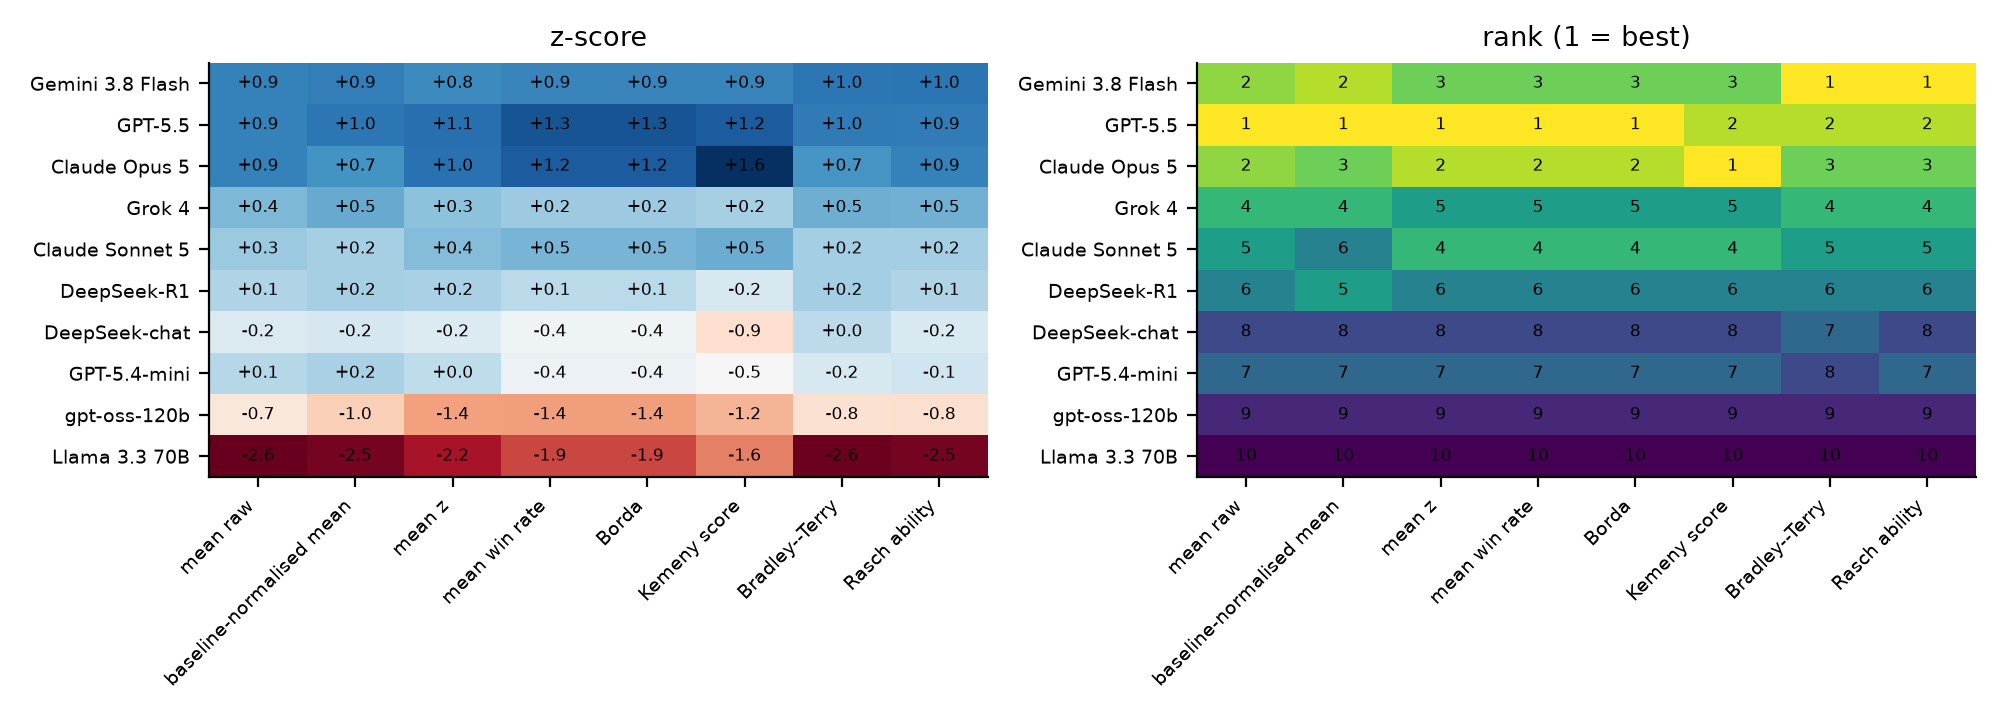
\includegraphics[width=0.85\textwidth]{fig_view_matrix.png}\caption{Each view's z-score (left) and rank (right) per model on native-metric scores.}\label{fig:fig_view_matrix}\end{figure}
\begin{figure}[htbp]\centering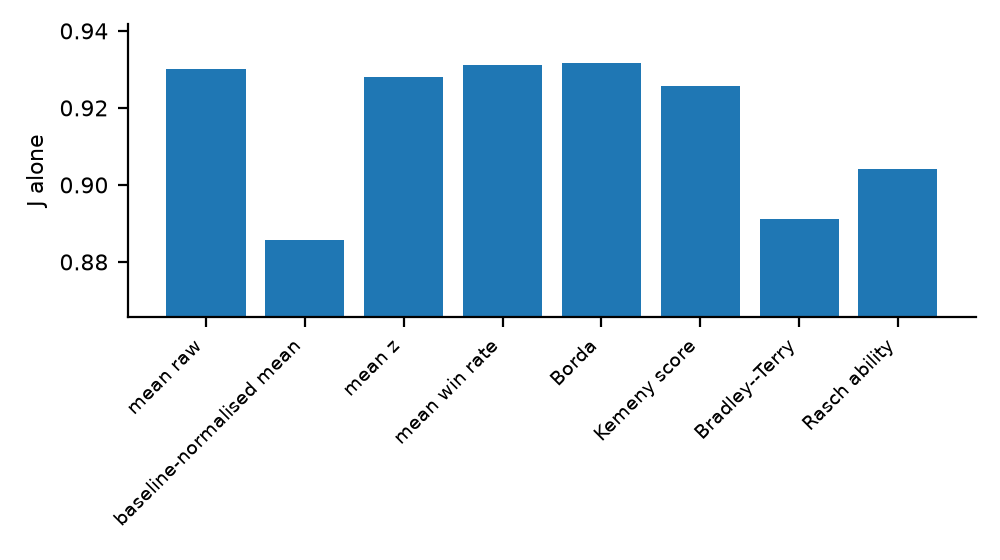
\includegraphics[width=0.6\textwidth]{fig_single_view_j.png}\caption{Objective $J$ of each view used alone.}\label{fig:fig_single_view_j}\end{figure}
\begin{figure}[htbp]\centering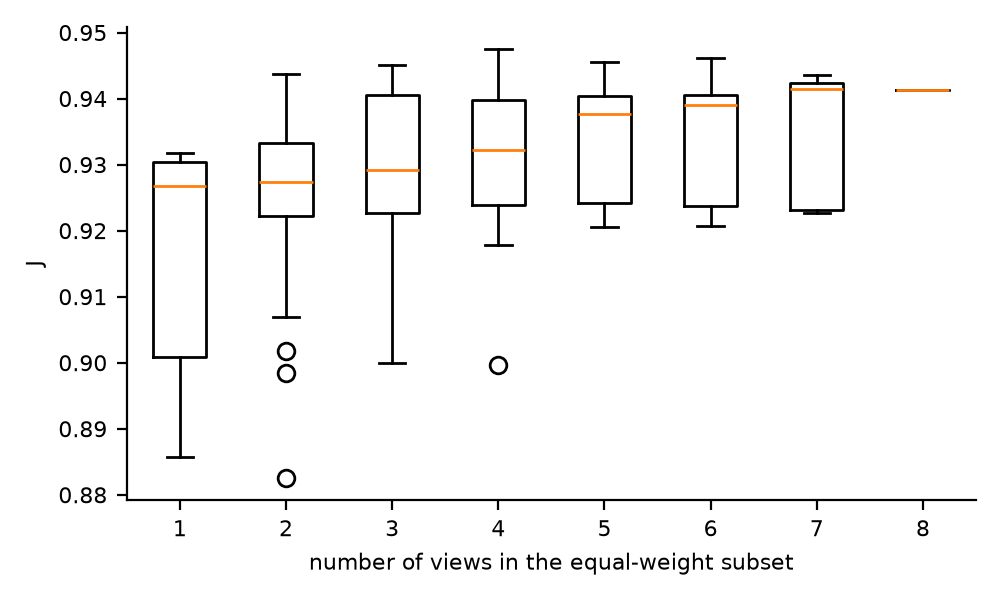
\includegraphics[width=0.6\textwidth]{fig_j_by_subset_size.png}\caption{Objective $J$ of the 255 equal-weight subsets by subset size.}\label{fig:fig_j_by_subset_size}\end{figure}
\begin{figure}[htbp]\centering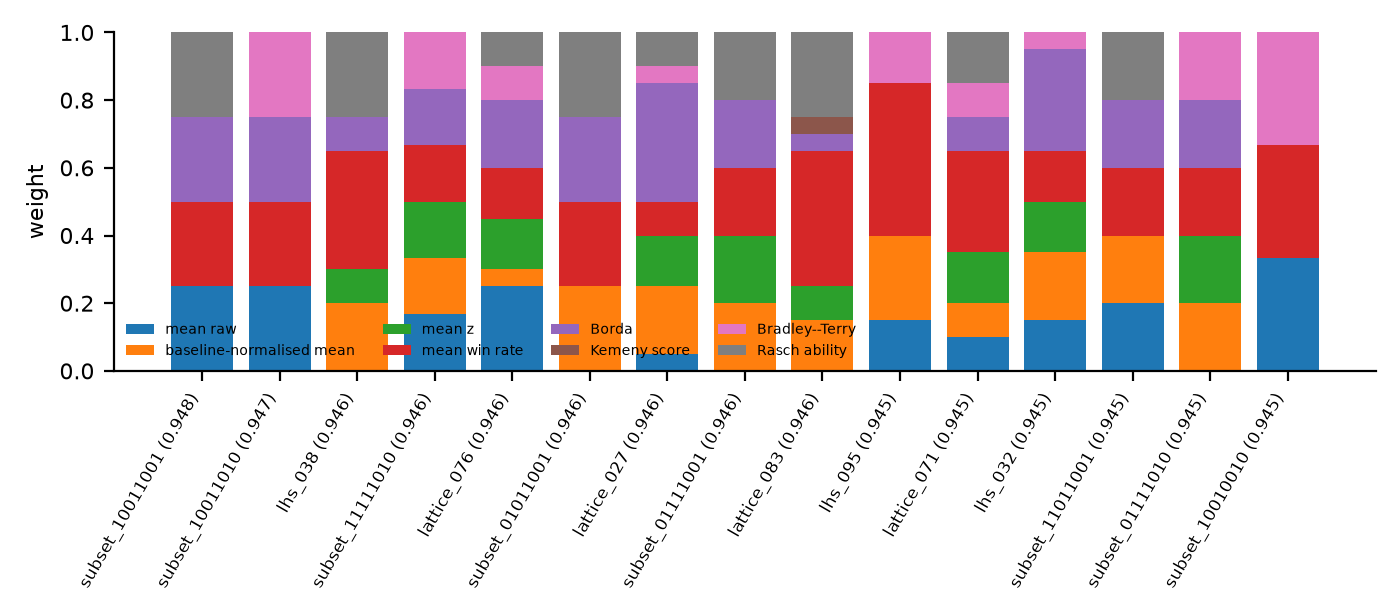
\includegraphics[width=0.85\textwidth]{fig_top_mix_weights.png}\caption{View weights of the fifteen best candidate mixes (label and $J$ on the axis).}\label{fig:fig_top_mix_weights}\end{figure}
\begin{landscape}
\begin{table}[htbp]
\centering\tiny
\caption{The fifteen best candidate mixes with their weights and objective terms.}
\label{tab:top_mixes}
\setlength{\tabcolsep}{3pt}
\resizebox{\linewidth}{!}{%
\begin{tabular}{lrrrrrrrrrrrrrr}
\toprule
rank & label & n\_\allowbreak{}views & w\_\allowbreak{}mean\_\allowbreak{}raw & w\_\allowbreak{}baseline\_\allowbreak{}norm\_\allowbreak{}mean & w\_\allowbreak{}z\_\allowbreak{}mean & w\_\allowbreak{}mean\_\allowbreak{}win\_\allowbreak{}rate & w\_\allowbreak{}borda & w\_\allowbreak{}kemeny\_\allowbreak{}score & w\_\allowbreak{}bradley\_\allowbreak{}terry & w\_\allowbreak{}irt\_\allowbreak{}ability & stability & transitivity & reference & J \\
\midrule
1 & subset\_\allowbreak{}10011001 & 4 & 0.250 & 0.000 & 0.000 & 0.250 & 0.250 & 0.000 & 0.000 & 0.250 & 0.923 & 0.944 & 1.000 & 0.948 \\
2 & subset\_\allowbreak{}10011010 & 4 & 0.250 & 0.000 & 0.000 & 0.250 & 0.250 & 0.000 & 0.250 & 0.000 & 0.923 & 0.944 & 1.000 & 0.947 \\
3 & lhs\_\allowbreak{}038 & 5 & 0.000 & 0.200 & 0.100 & 0.350 & 0.100 & 0.000 & 0.000 & 0.250 & 0.920 & 0.944 & 1.000 & 0.946 \\
4 & subset\_\allowbreak{}11111010 & 6 & 0.167 & 0.167 & 0.167 & 0.167 & 0.167 & 0.000 & 0.167 & 0.000 & 0.920 & 0.944 & 1.000 & 0.946 \\
5 & lattice\_\allowbreak{}076 & 7 & 0.250 & 0.050 & 0.150 & 0.150 & 0.200 & 0.000 & 0.100 & 0.100 & 0.920 & 0.944 & 1.000 & 0.946 \\
6 & subset\_\allowbreak{}01011001 & 4 & 0.000 & 0.250 & 0.000 & 0.250 & 0.250 & 0.000 & 0.000 & 0.250 & 0.920 & 0.944 & 1.000 & 0.946 \\
7 & lattice\_\allowbreak{}027 & 7 & 0.050 & 0.200 & 0.150 & 0.100 & 0.350 & 0.000 & 0.050 & 0.100 & 0.920 & 0.944 & 1.000 & 0.946 \\
8 & subset\_\allowbreak{}01111001 & 5 & 0.000 & 0.200 & 0.200 & 0.200 & 0.200 & 0.000 & 0.000 & 0.200 & 0.919 & 0.944 & 1.000 & 0.946 \\
9 & lattice\_\allowbreak{}083 & 6 & 0.000 & 0.150 & 0.100 & 0.400 & 0.050 & 0.050 & 0.000 & 0.250 & 0.919 & 0.944 & 1.000 & 0.946 \\
12 & lhs\_\allowbreak{}095 & 4 & 0.150 & 0.250 & 0.000 & 0.450 & 0.000 & 0.000 & 0.150 & 0.000 & 0.919 & 0.944 & 1.000 & 0.945 \\
11 & lattice\_\allowbreak{}071 & 7 & 0.100 & 0.100 & 0.150 & 0.300 & 0.100 & 0.000 & 0.100 & 0.150 & 0.919 & 0.944 & 1.000 & 0.945 \\
10 & lhs\_\allowbreak{}032 & 6 & 0.150 & 0.200 & 0.150 & 0.150 & 0.300 & 0.000 & 0.050 & 0.000 & 0.919 & 0.944 & 1.000 & 0.945 \\
13 & subset\_\allowbreak{}11011001 & 5 & 0.200 & 0.200 & 0.000 & 0.200 & 0.200 & 0.000 & 0.000 & 0.200 & 0.918 & 0.944 & 1.000 & 0.945 \\
14 & subset\_\allowbreak{}01111010 & 5 & 0.000 & 0.200 & 0.200 & 0.200 & 0.200 & 0.000 & 0.200 & 0.000 & 0.918 & 0.944 & 1.000 & 0.945 \\
15 & subset\_\allowbreak{}10010010 & 3 & 0.333 & 0.000 & 0.000 & 0.333 & 0.000 & 0.000 & 0.333 & 0.000 & 0.918 & 0.944 & 1.000 & 0.945 \\
\bottomrule
\end{tabular}
}
\end{table}
\end{landscape}



\subsection{Honest selection}
The split-half test (Figure~\ref{fig:fig_split_half}) is the honesty check for the choice of mix. The mix selected on half A loses 0.032 of $J$ on half B, and 20 splits select 10 different mixes. On the held-out half the selected mix beats pure Bradley--Terry by +0.024 with an interval that includes zero, and the plain uniform mix (0.917) does as well as the selected one (0.903). Mixing views is therefore defensible but not demonstrably better than the uniform mix; pure Bradley--Terry is the least reproducible single rule on this suite.
\begin{figure}[htbp]\centering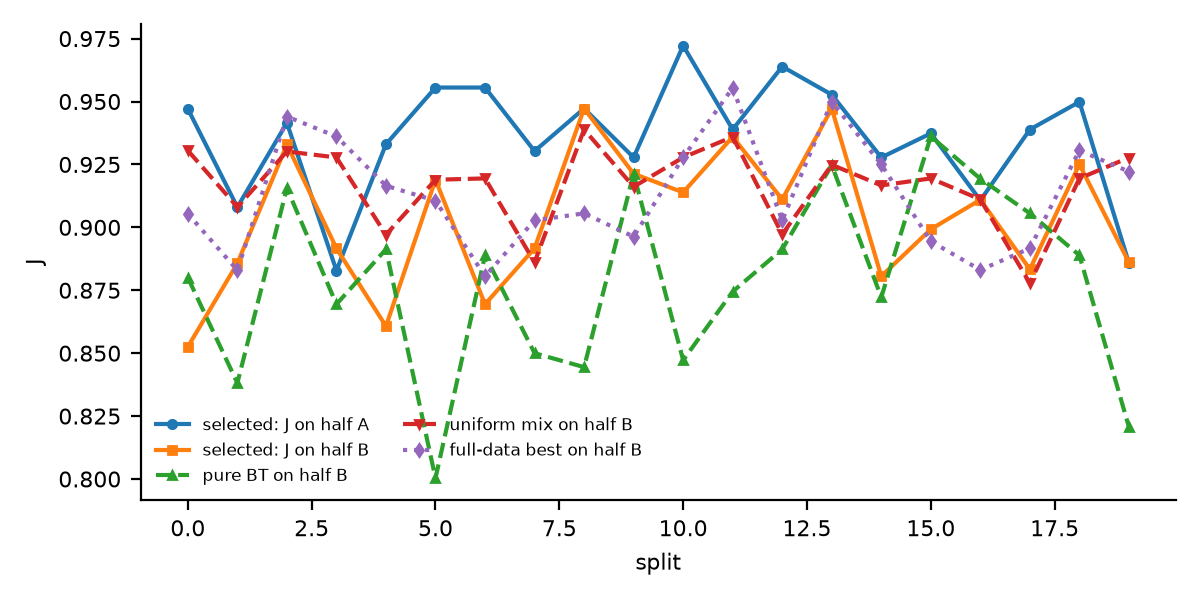
\includegraphics[width=0.85\textwidth]{fig_split_half.png}\caption{Split-half honesty check: the mix selected on half A scored on both halves, against pure Bradley--Terry, the uniform mix and the full-data best on half B.}\label{fig:fig_split_half}\end{figure}
\begin{table}[htbp]
\centering\scriptsize
\caption{Split-half summary.}
\label{tab:split_half_summary}
\setlength{\tabcolsep}{3pt}
\begin{tabular}{p{0.156\linewidth}p{0.786\linewidth}}
\toprule
quantity & value \\
\midrule
splits & 20 \\
inner\_\allowbreak{}resamples & 8 \\
J\_\allowbreak{}A\_\allowbreak{}selected\_\allowbreak{}mean & 0.935 \\
J\_\allowbreak{}B\_\allowbreak{}selected\_\allowbreak{}mean & 0.903 \\
optimism\_\allowbreak{}gap & 0.032 \\
J\_\allowbreak{}B\_\allowbreak{}pure\_\allowbreak{}bt\_\allowbreak{}mean & 0.879 \\
J\_\allowbreak{}B\_\allowbreak{}uniform\_\allowbreak{}mean & 0.917 \\
J\_\allowbreak{}B\_\allowbreak{}full\_\allowbreak{}best\_\allowbreak{}mean & 0.913 \\
selected\_\allowbreak{}minus\_\allowbreak{}pure\_\allowbreak{}bt & {"mean": 0.02427983120362126, "ci95": [-0.03387181157278865, 0.11109314599900576], "share\_\allowbreak{}selected\_\allowbreak{}ahead": 0.7} \\
\bottomrule
\end{tabular}
\end{table}



\subsection{Parameters with standard errors}
Table~\ref{tab:parameters} and Figure~\ref{fig:fig_parameters} give the fitted Bradley--Terry strengths and Rasch abilities. The analytic standard errors assume the model is right; the bootstrap SDs (Figure~\ref{fig:fig_parameter_bootstrap}) do not, and with ten models they are the ones to quote. Rasch item difficulties are poorly determined (mean SE 7.4, Figure~\ref{fig:fig_rasch_items}): with ten responses per item the one-parameter model cannot pin individual items down, which is why the Rasch view is the least stable.
\begin{landscape}
\begin{table}[htbp]
\centering\tiny
\caption{Fitted parameters with standard errors (native metric). Kemeny cost 329 of 1395.}
\label{tab:parameters}
\setlength{\tabcolsep}{3pt}
\resizebox{\linewidth}{!}{%
\begin{tabular}{lrrrrrrrr}
\toprule
model & BT strength & BT SE vs ref & BT bootstrap SD & Rasch ability & Rasch SE & Rasch bootstrap SD & Copeland & Kemeny position \\
\midrule
Gemini 3.8 Flash & 0.063 & 0.016 & 0.005 & 0.736 & 0.104 & 0.078 & 6.500 & 3 \\
GPT-5.5 & 0.060 & 0.016 & 0.005 & 0.693 & 0.103 & 0.075 & 7.500 & 2 \\
Claude Opus 5 & 0.045 & 0.000 & 0.005 & 0.651 & 0.103 & 0.086 & 8.500 & 1 \\
Grok 4 & 0.031 & 0.016 & 0.005 & 0.345 & 0.099 & 0.067 & 4.500 & 5 \\
Claude Sonnet 5 & 0.012 & 0.016 & 0.005 & 0.125 & 0.097 & 0.067 & 4.500 & 4 \\
DeepSeek-R1 & 0.012 & 0.016 & 0.005 & 0.070 & 0.096 & 0.070 & 3.500 & 6 \\
DeepSeek-chat & 0.002 & 0.016 & 0.005 & -0.155 & 0.094 & 0.067 & 1.500 & 8 \\
GPT-5.4-mini & -0.011 & 0.016 & 0.005 & -0.084 & 0.094 & 0.066 & 2.500 & 7 \\
gpt-oss-120b & -0.053 & 0.016 & 0.006 & -0.608 & 0.090 & 0.069 & 0.500 & 9 \\
Llama 3.3 70B & -0.161 & 0.016 & 0.007 & -1.775 & 0.085 & 0.083 & -0.500 & 10 \\
\bottomrule
\end{tabular}
}
\end{table}
\end{landscape}

\begin{figure}[htbp]\centering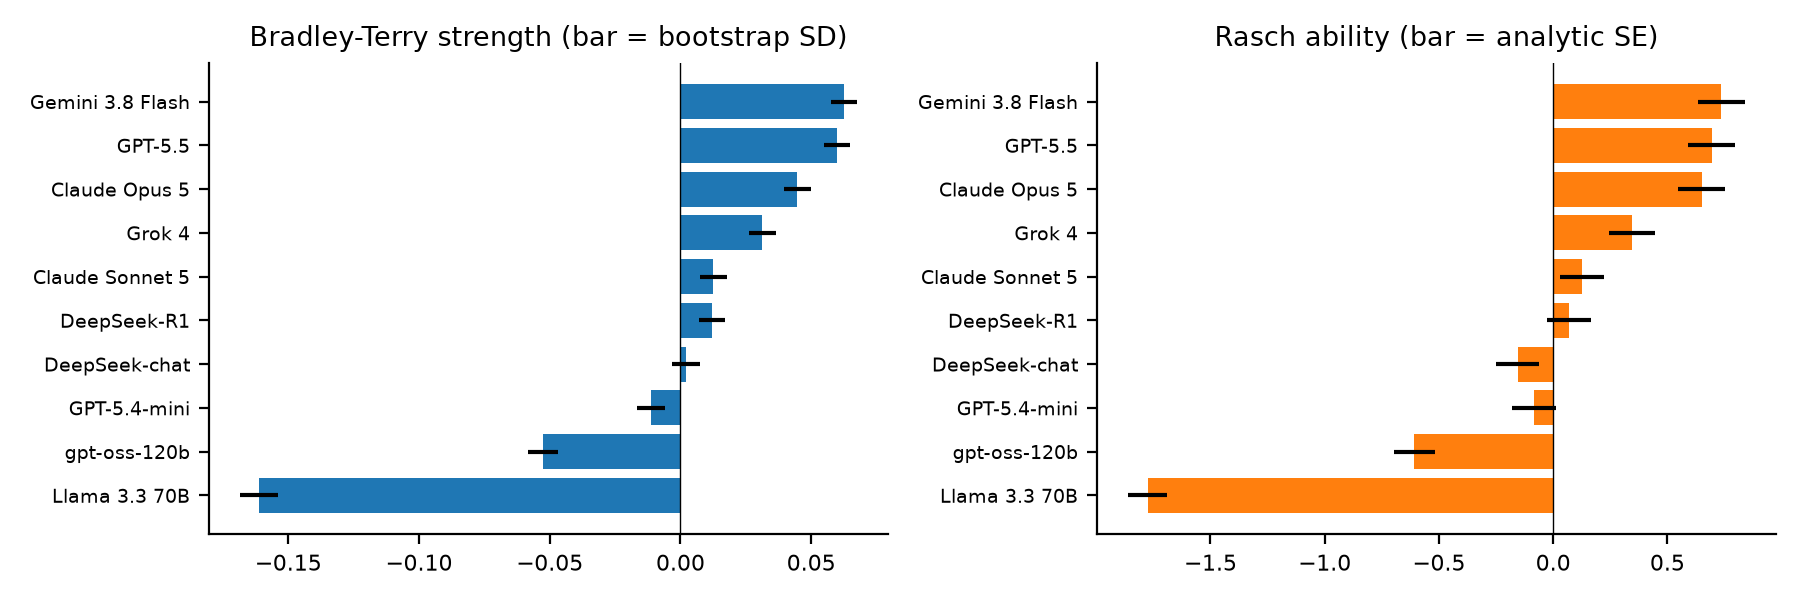
\includegraphics[width=0.85\textwidth]{fig_parameters.png}\caption{Fitted Bradley--Terry strengths and Rasch abilities with their uncertainty.}\label{fig:fig_parameters}\end{figure}
\begin{figure}[htbp]\centering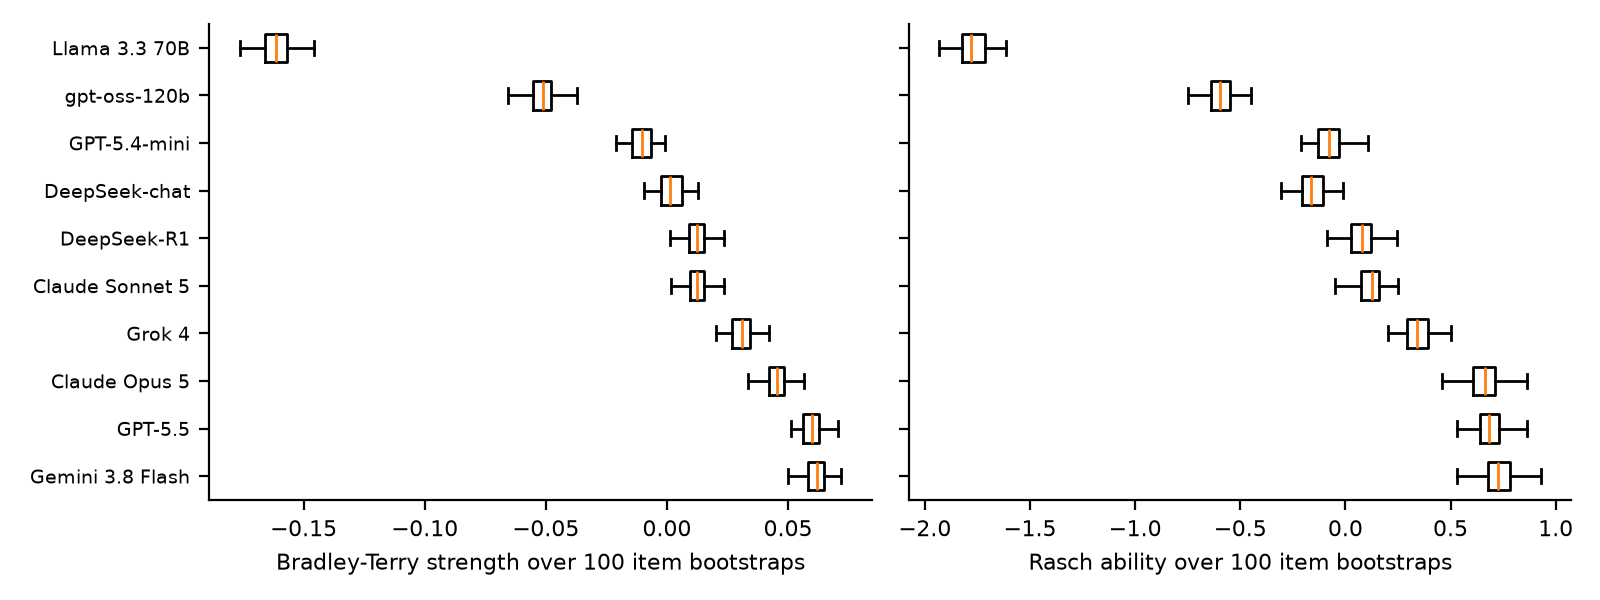
\includegraphics[width=0.85\textwidth]{fig_parameter_bootstrap.png}\caption{Bootstrap distributions of the Bradley--Terry strengths and Rasch abilities (100 item resamples).}\label{fig:fig_parameter_bootstrap}\end{figure}


\subsection{Leaderboard}
Under the native metric pooled by Bradley--Terry, Gemini 3.8 Flash is first ($P(\text{first}) = 0.62$) with GPT-5.5 and Claude Opus 5 next; Borda puts GPT-5.5 first. Exact match puts Claude Opus 5 first. The ends are fixed under every rule and pooling method; Friedman rejects equal models ($p$ = 1.2e-13) while datasets agree only moderately ($W$ = 0.27).
\begin{table}[htbp]
\centering\tiny
\caption{Leaderboard under the headline rule (native metric).}
\label{tab:leaderboard_headline}
\setlength{\tabcolsep}{3pt}
\begin{tabular}{lp{0.256\linewidth}p{0.176\linewidth}rrrp{0.176\linewidth}r}
\toprule
rank & model & BT strength & SE & Borda rank & Borda 95\% & P(first) BT & mean score \\
\midrule
1 & Gemini 3.8 Flash & 0.063 & 0.016 & 3 & [2, 4] & 0.620 & 0.792 \\
2 & GPT-5.5 & 0.060 & 0.016 & 1 & [1, 3] & 0.370 & 0.793 \\
3 & Claude Opus 5 & 0.045 & 0.000 & 2 & [1, 3] & 0.000 & 0.792 \\
4 & Grok 4 & 0.031 & 0.016 & 5 & [3, 6] & 0.000 & 0.780 \\
5 & Claude Sonnet 5 & 0.012 & 0.016 & 4 & [3, 6] & 0.000 & 0.776 \\
6 & DeepSeek-R1 & 0.012 & 0.016 & 6 & [4, 8] & 0.000 & 0.772 \\
7 & DeepSeek-chat & 0.002 & 0.016 & 8 & [6, 8] & 0.000 & 0.763 \\
8 & GPT-5.4-mini & -0.011 & 0.016 & 7 & [6, 8] & 0.000 & 0.771 \\
9 & gpt-oss-120b & -0.053 & 0.016 & 9 & [9, 9] & 0.000 & 0.750 \\
10 & Llama 3.3 70B & -0.161 & 0.016 & 10 & [10, 10] & 0.000 & 0.701 \\
\bottomrule
\end{tabular}
\end{table}

\begin{landscape}
\begin{table}[htbp]
\centering\tiny
\caption{Bradley--Terry rank (Borda rank in brackets) under each reported rule, Friedman $p$ and Kendall's $W$ among datasets.}
\label{tab:ranks_by_rule}
\setlength{\tabcolsep}{3pt}
\resizebox{\linewidth}{!}{%
\begin{tabular}{lrrrrrrrrrrrr}
\toprule
rule & Gemini 3.8 Flash & GPT-5.5 & Claude Opus 5 & Grok 4 & Claude Sonnet 5 & DeepSeek-R1 & DeepSeek-chat & GPT-5.4-mini & gpt-oss-120b & Llama 3.3 70B & Friedman p & W \\
\midrule
native metric & 1 (3) & 2 (1) & 3 (2) & 4 (5) & 5 (4) & 6 (6) & 7 (8) & 8 (7) & 9 (9) & 10 (10) & 1.2e-13 & 0.27 \\
exact match & 3 (3) & 2 (2) & 1 (1) & 4 (5) & 5 (4) & 7 (6) & 8 (7) & 6 (8) & 9 (9) & 10 (10) & 5.3e-14 & 0.28 \\
\bottomrule
\end{tabular}
}
\end{table}
\end{landscape}

\begin{figure}[htbp]\centering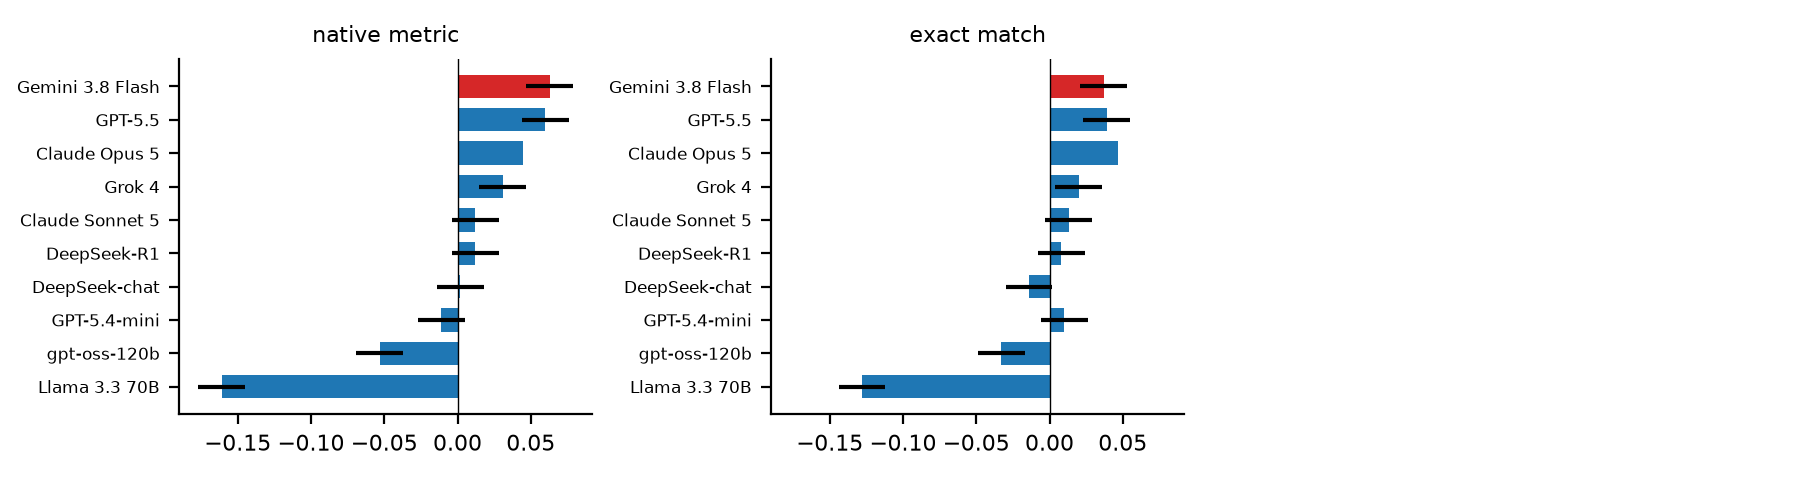
\includegraphics[width=0.85\textwidth]{fig_bt_all_rules.png}\caption{Bradley--Terry strengths ($\pm$ SE vs reference) under every reported rule; models fixed in the headline order.}\label{fig:fig_bt_all_rules}\end{figure}
\begin{figure}[htbp]\centering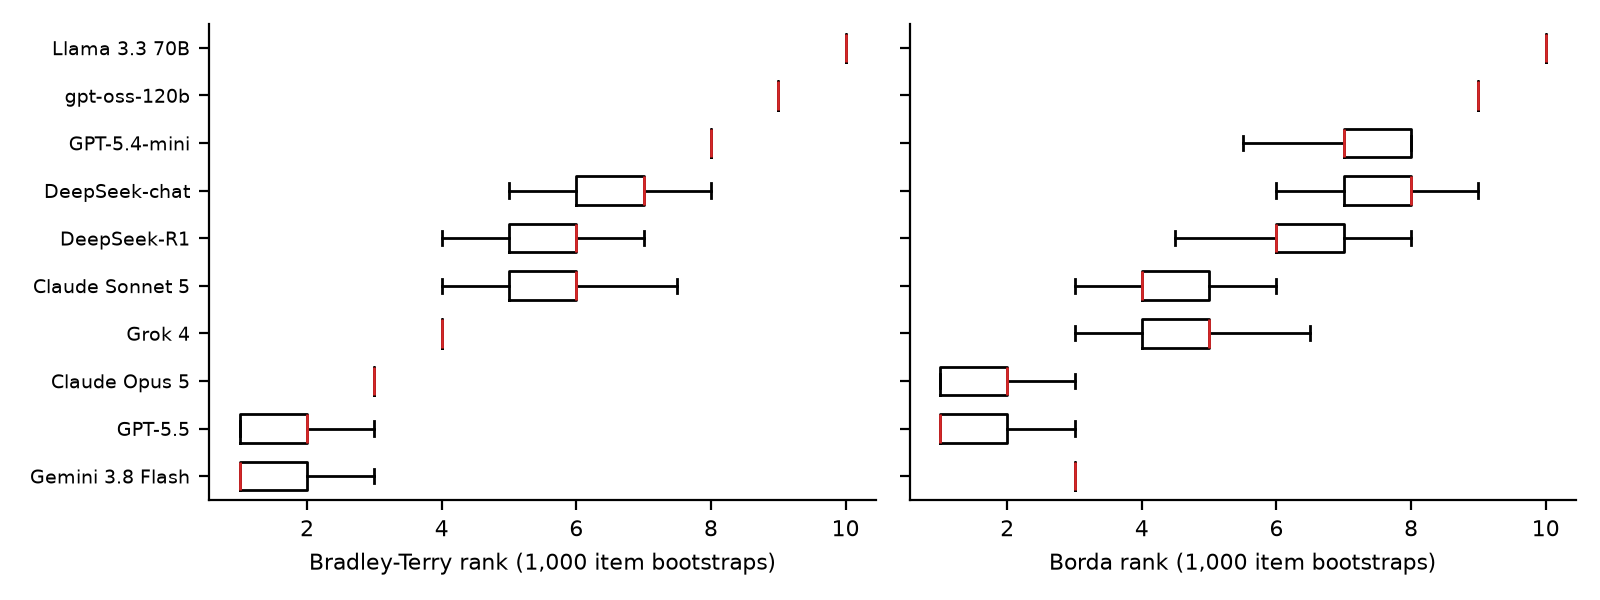
\includegraphics[width=0.85\textwidth]{fig_rank_bootstrap.png}\caption{Bootstrap distribution of each model's rank under the headline rule (native metric).}\label{fig:fig_rank_bootstrap}\end{figure}
\begin{figure}[htbp]\centering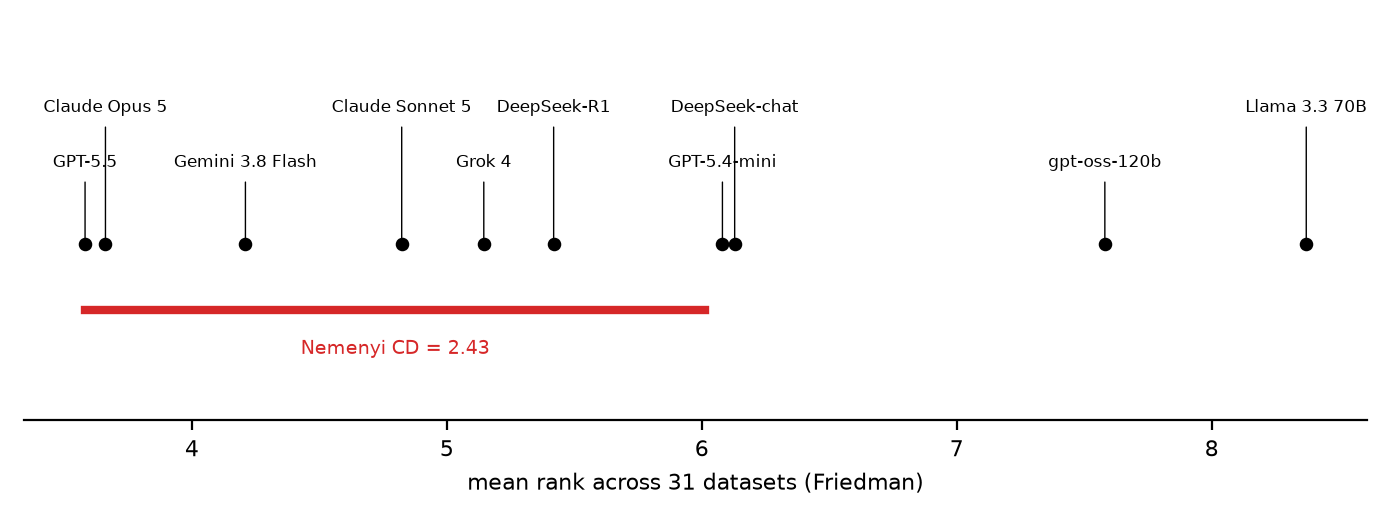
\includegraphics[width=0.85\textwidth]{fig_cd_diagram.png}\caption{Critical-difference view of the Friedman test under the headline rule: mean rank per model and the Nemenyi critical difference at $\alpha=.05$.}\label{fig:fig_cd_diagram}\end{figure}


\subsection{Comparability and diagnostics}
\begin{table}[htbp]
\centering\tiny
\caption{Official-split estimates under the headline rule averaged over the ten models.}
\label{tab:official_split_by_dataset}
\setlength{\tabcolsep}{3pt}
\begin{tabular}{p{0.121\linewidth}rp{0.108\linewidth}p{0.076\linewidth}p{0.140\linewidth}p{0.121\linewidth}p{0.095\linewidth}p{0.146\linewidth}}
\toprule
dataset & suite\_\allowbreak{}mean & official\_\allowbreak{}estimate & suite\_\allowbreak{}f1\_\allowbreak{}pos & official\_\allowbreak{}precision\_\allowbreak{}pos & official\_\allowbreak{}recall\_\allowbreak{}pos & official\_\allowbreak{}f1\_\allowbreak{}pos & official\_\allowbreak{}positive\_\allowbreak{}share \\
\midrule
abt\_\allowbreak{}buy & 0.970 & 0.986 & 0.968 & 0.926 & 0.949 & 0.936 & 0.108 \\
alaska\_\allowbreak{}camera & 0.958 & 0.958 & 0.955 & 1.000 & 0.921 & 0.955 & 0.500 \\
alaska\_\allowbreak{}schema & 0.897 & 0.897 & -- & -- & -- & -- & -- \\
amazon\_\allowbreak{}google & 0.936 & 0.932 & 0.929 & 0.611 & 0.942 & 0.739 & 0.102 \\
bird & 0.126 & 0.157 & -- & -- & -- & -- & -- \\
dblp\_\allowbreak{}acm & 0.986 & 0.991 & 0.985 & 0.979 & 0.978 & 0.976 & 0.180 \\
dblp\_\allowbreak{}scholar & 0.949 & 0.966 & 0.948 & 0.900 & 0.924 & 0.910 & 0.186 \\
fetaqa & 0.468 & 0.468 & -- & -- & -- & -- & -- \\
fintagging & 0.794 & 0.789 & -- & -- & -- & -- & -- \\
hitab & 0.743 & 0.759 & -- & -- & -- & -- & -- \\
machamp & 0.887 & 0.890 & 0.892 & 0.644 & 0.853 & 0.733 & 0.175 \\
magneto\_\allowbreak{}gdc & 0.908 & 0.911 & -- & -- & -- & -- & -- \\
mmtu & 0.879 & 0.834 & -- & -- & -- & -- & -- \\
officeqa & 0.077 & 0.077 & -- & -- & -- & -- & -- \\
officeqa\_\allowbreak{}pro\_\allowbreak{}v2 & 0.082 & 0.082 & -- & -- & -- & -- & -- \\
opensanctions\_\allowbreak{}pairs & 0.821 & 0.727 & 0.773 & 0.993 & 0.649 & 0.777 & 0.769 \\
papadakis\_\allowbreak{}dn & 0.941 & 0.988 & 0.833 & 0.550 & 0.963 & 0.683 & 0.018 \\
realhitbench & 0.630 & 0.628 & -- & -- & -- & -- & -- \\
smat & 0.876 & 0.873 & -- & -- & -- & -- & -- \\
suc & 0.886 & 0.882 & -- & -- & -- & -- & -- \\
tab\_\allowbreak{}fact & 0.798 & 0.789 & 0.758 & 0.896 & 0.674 & 0.764 & 0.500 \\
tabis & 0.915 & 0.918 & -- & -- & -- & -- & -- \\
tablebench & 0.802 & 0.800 & -- & -- & -- & -- & -- \\
tableeval & 0.720 & 0.731 & -- & -- & -- & -- & -- \\
tat\_\allowbreak{}qa & 0.751 & 0.706 & -- & -- & -- & -- & -- \\
tpcdi\_\allowbreak{}cells & 0.343 & 0.375 & -- & -- & -- & -- & -- \\
valentine & 0.979 & 0.971 & -- & -- & -- & -- & -- \\
walmart\_\allowbreak{}amazon & 0.958 & 0.975 & 0.947 & 0.832 & 0.927 & 0.875 & 0.094 \\
wdc\_\allowbreak{}lspc & 0.982 & 0.983 & 0.983 & 0.965 & 0.979 & 0.971 & 0.264 \\
wdc\_\allowbreak{}products & 0.978 & 0.985 & 0.979 & 0.980 & 0.968 & 0.974 & 0.280 \\
wikitablequestions & 0.799 & 0.796 & -- & -- & -- & -- & -- \\
\bottomrule
\end{tabular}
\end{table}

\begin{figure}[htbp]\centering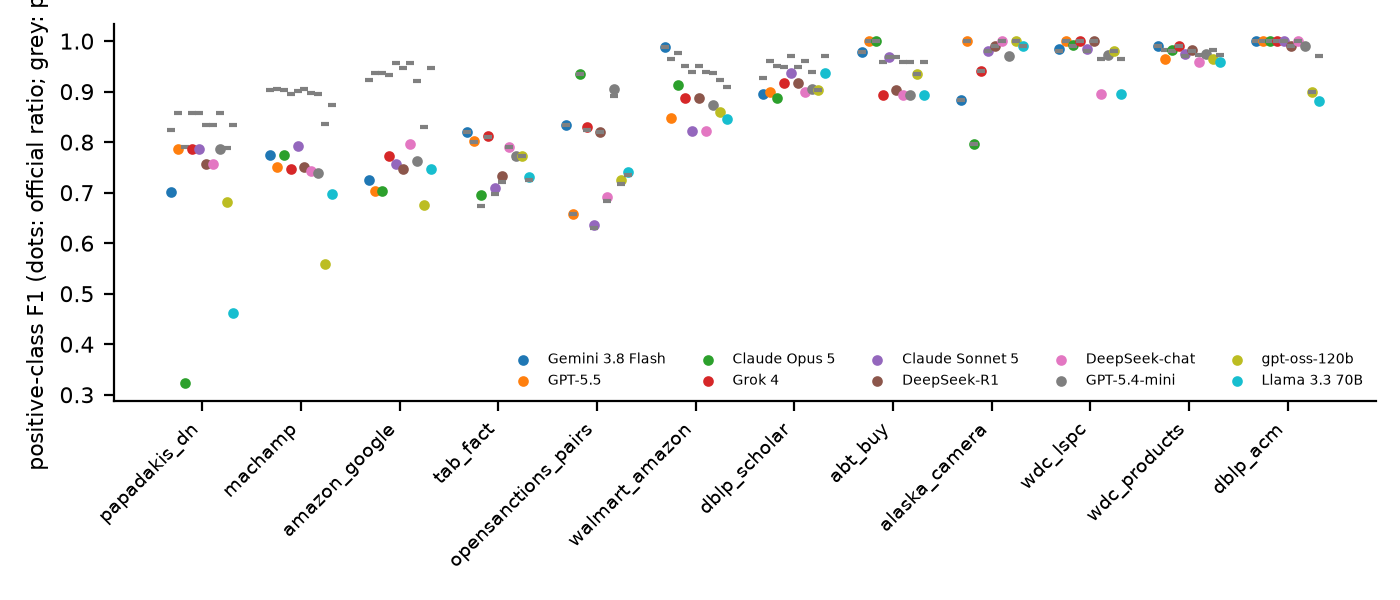
\includegraphics[width=0.85\textwidth]{fig_official_f1_models.png}\caption{Positive-class F1 on the balanced pool (grey) and at the official match ratio (coloured) per model and matching dataset.}\label{fig:fig_official_f1_models}\end{figure}
\begin{figure}[htbp]\centering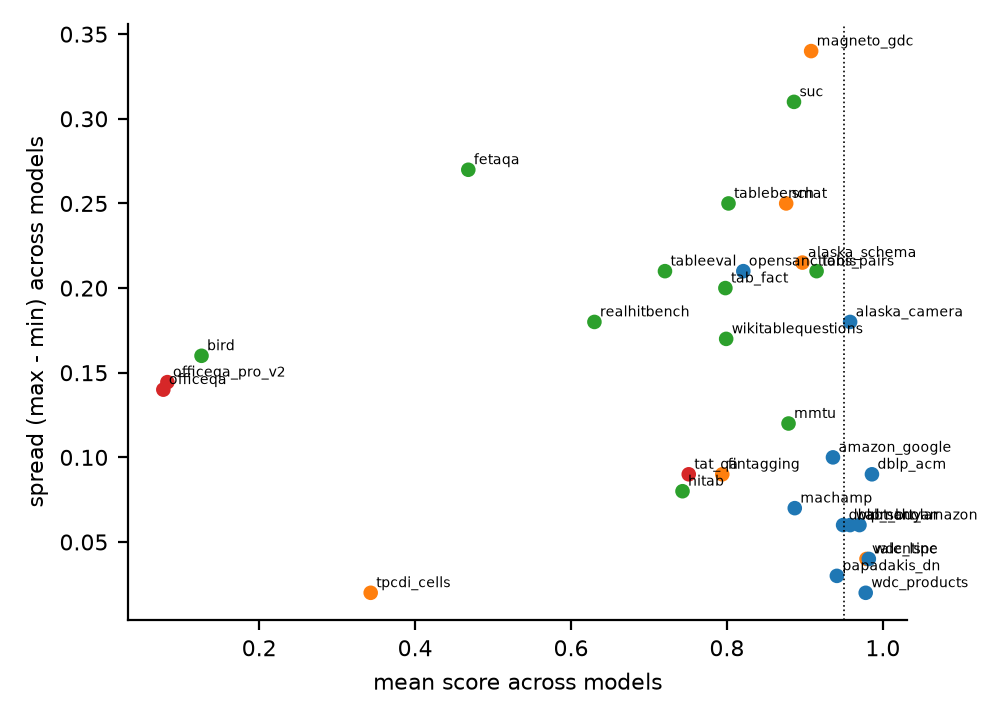
\includegraphics[width=0.6\textwidth]{fig_diagnostics_scatter.png}\caption{Dataset diagnostics: mean score against spread across models; dotted line marks the ceiling flag.}\label{fig:fig_diagnostics_scatter}\end{figure}


\clearpage
\appendix
\section{All figures}
Every figure that can be drawn from the saved outputs; source data in \texttt{data/}.
\begin{figure}[htbp]\centering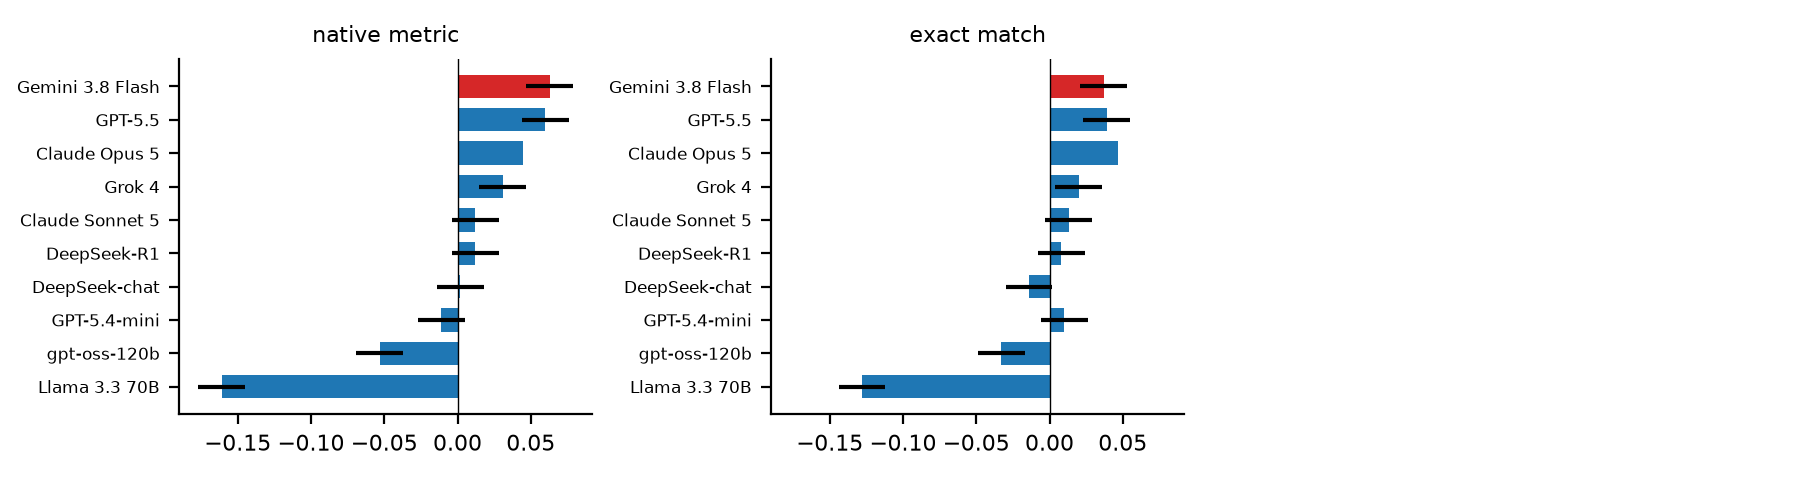
\includegraphics[width=0.9\textwidth]{fig_bt_all_rules.png}\caption{Bradley--Terry strengths ($\pm$ SE vs reference) under every reported rule; models fixed in the headline order.}\label{figall:fig_bt_all_rules}\end{figure}
\begin{figure}[htbp]\centering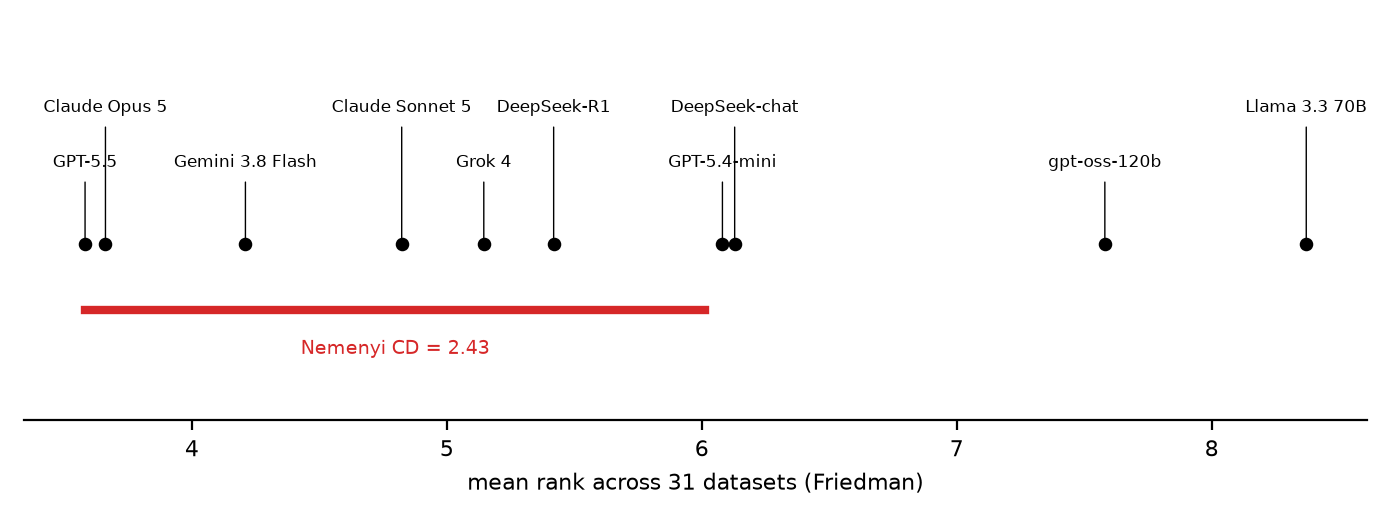
\includegraphics[width=0.9\textwidth]{fig_cd_diagram.png}\caption{Critical-difference view of the Friedman test under the headline rule: mean rank per model and the Nemenyi critical difference at $\alpha=.05$.}\label{figall:fig_cd_diagram}\end{figure}
\begin{figure}[htbp]\centering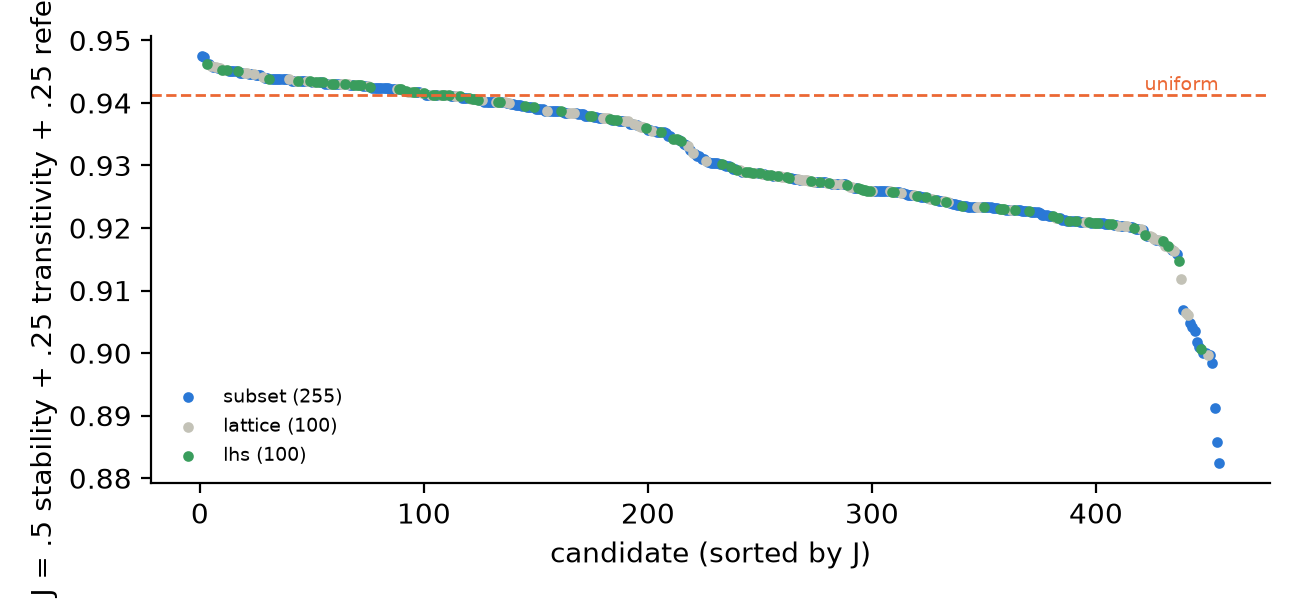
\includegraphics[width=0.9\textwidth]{fig_combos.png}\caption{All 455 candidate mixes sorted by $J$, coloured by design.}\label{figall:fig_combos}\end{figure}
\begin{figure}[htbp]\centering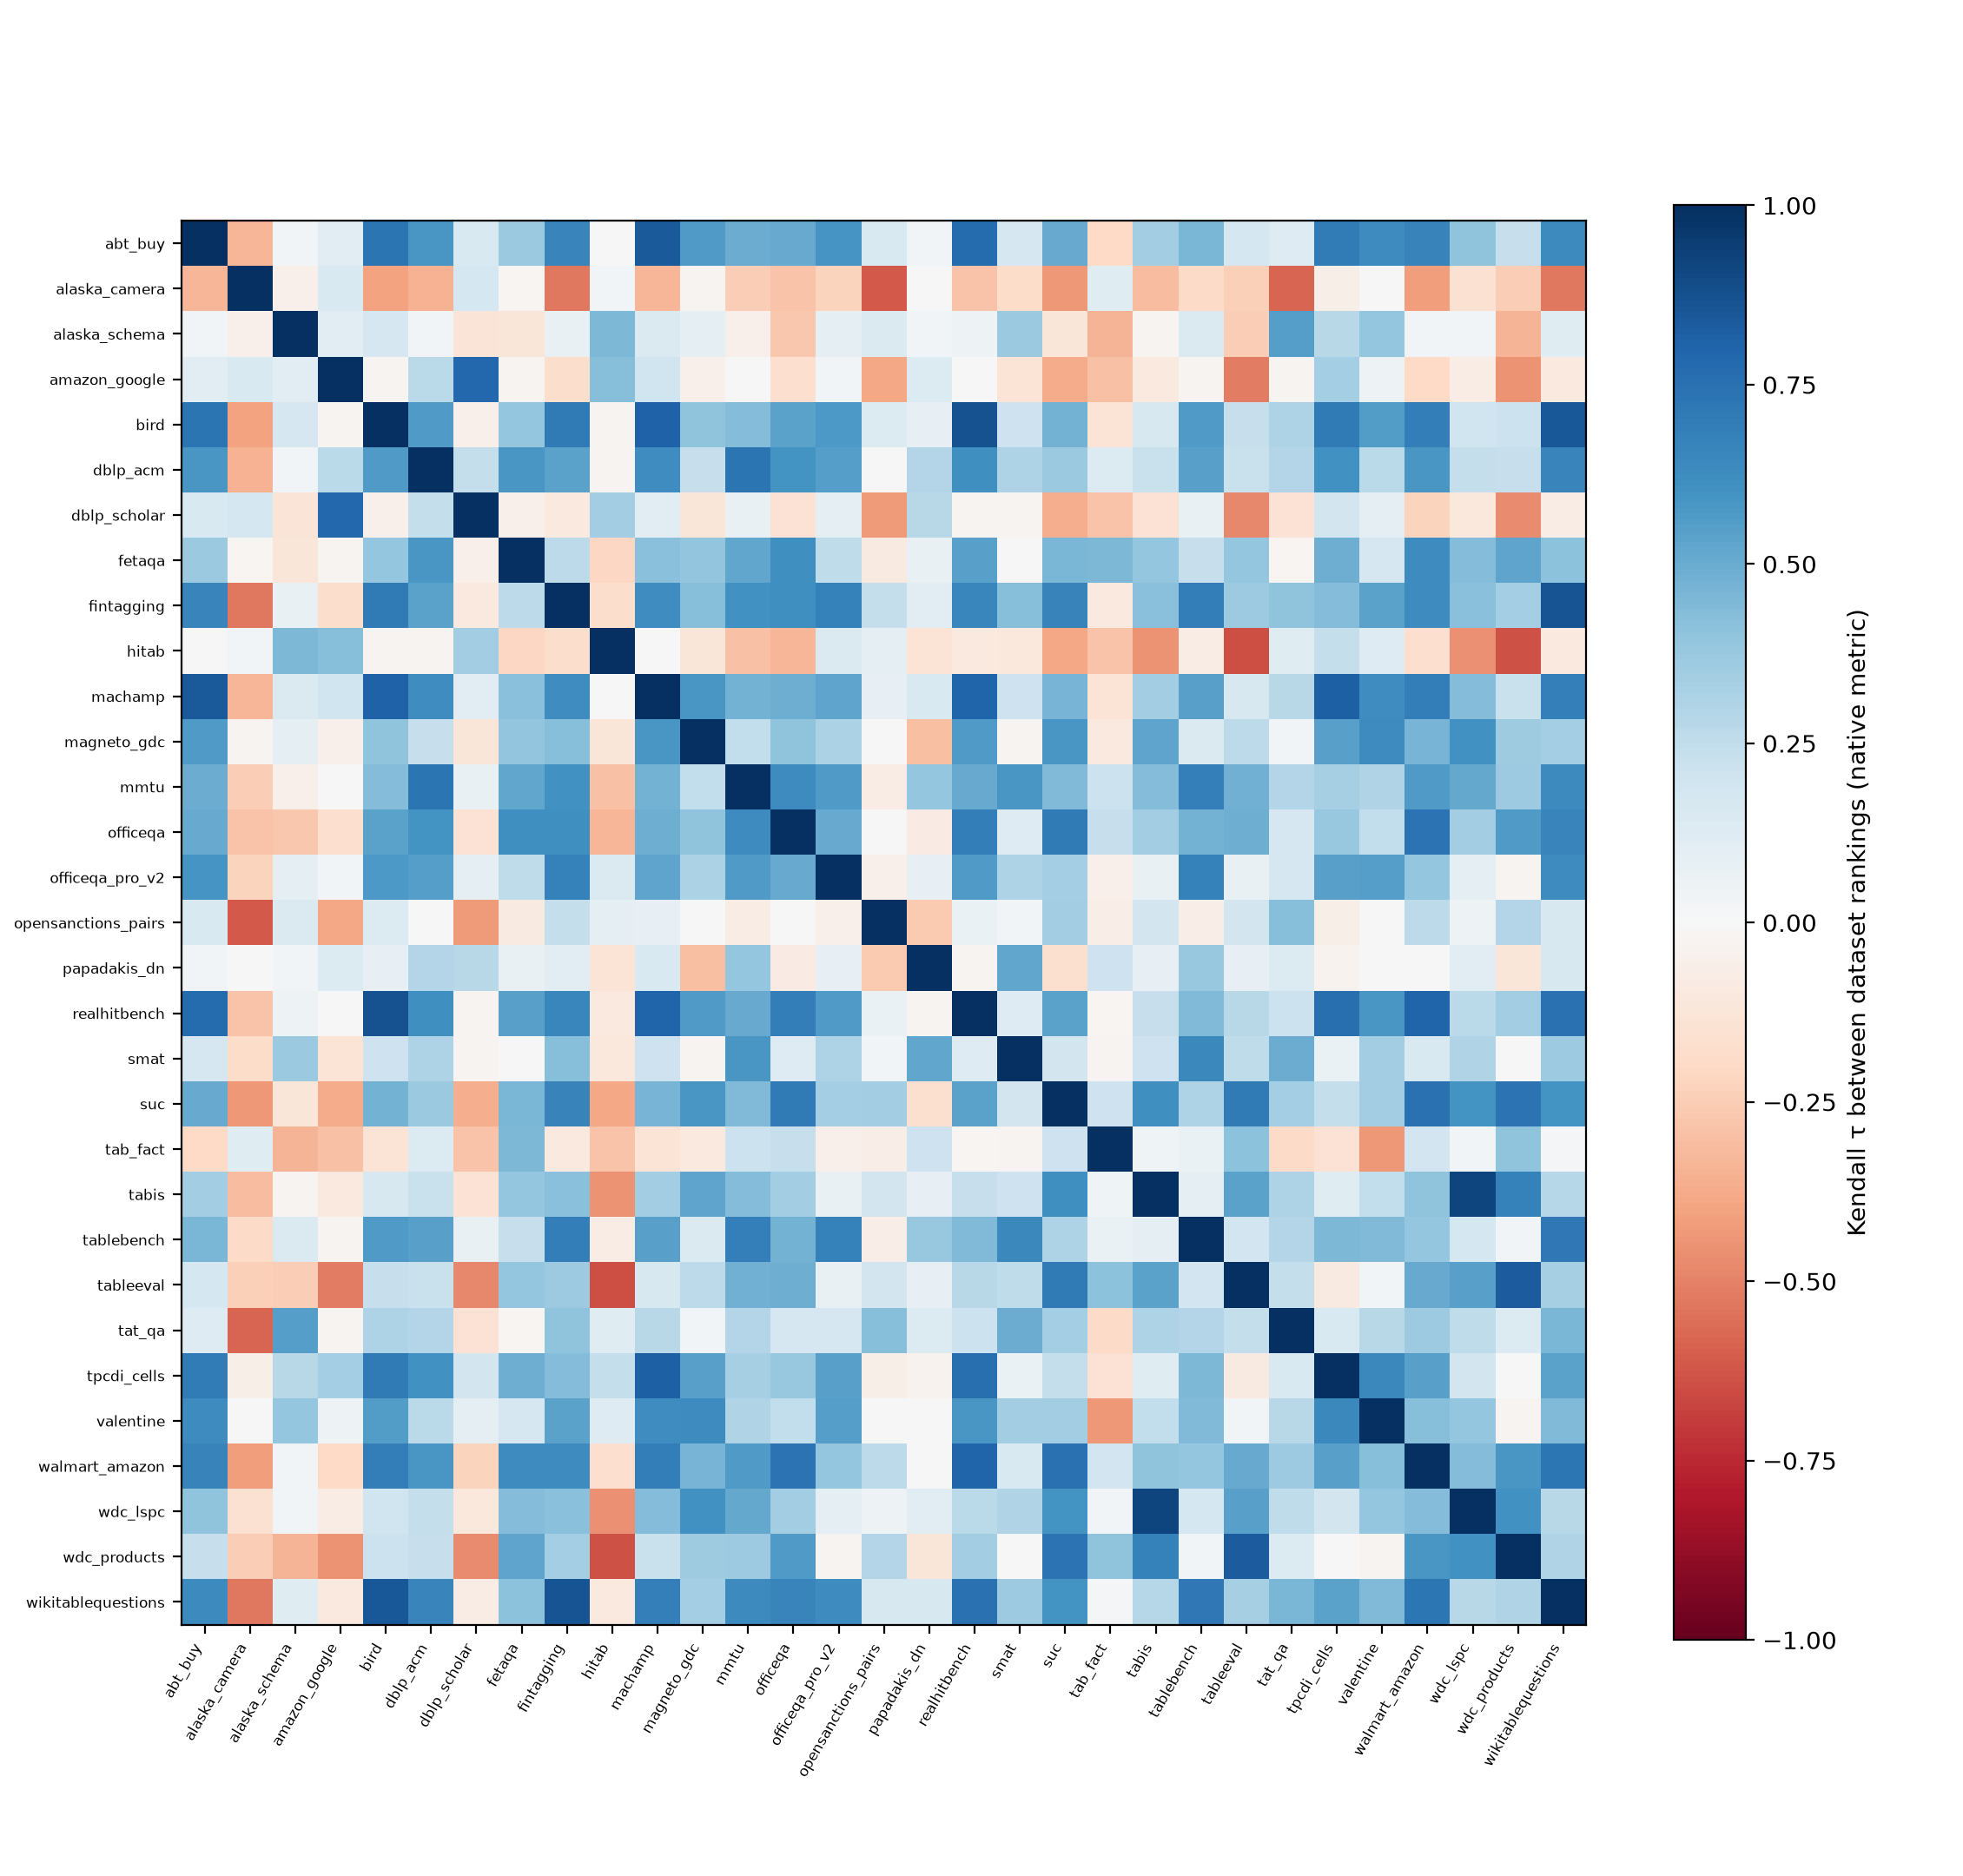
\includegraphics[width=0.9\textwidth]{fig_dataset_tau.png}\caption{Kendall $\tau$ between the model rankings of each pair of datasets under the headline rule.}\label{figall:fig_dataset_tau}\end{figure}
\begin{figure}[htbp]\centering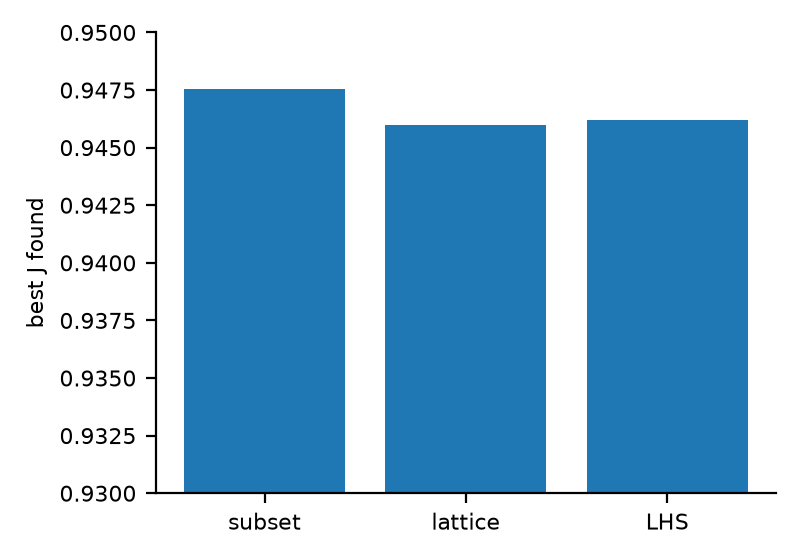
\includegraphics[width=0.9\textwidth]{fig_designs_v3.png}\caption{Best $J$ found by the enumerated subsets and the two sampled designs of 100 mixes each.}\label{figall:fig_designs_v3}\end{figure}
\begin{figure}[htbp]\centering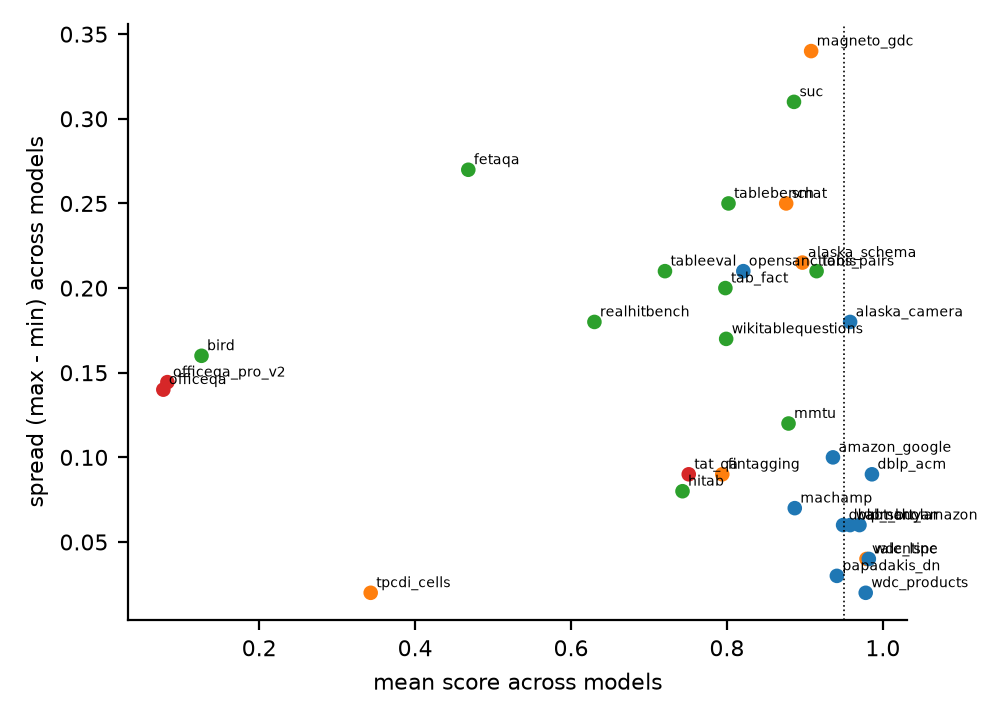
\includegraphics[width=0.9\textwidth]{fig_diagnostics_scatter.png}\caption{Dataset diagnostics: mean score against spread across models; dotted line marks the ceiling flag.}\label{figall:fig_diagnostics_scatter}\end{figure}
\begin{figure}[htbp]\centering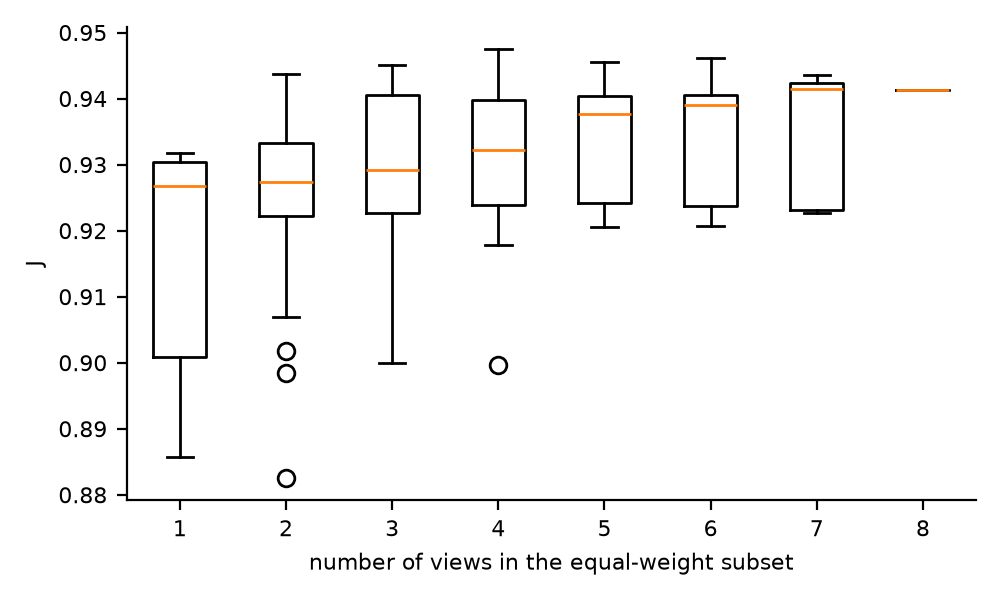
\includegraphics[width=0.9\textwidth]{fig_j_by_subset_size.png}\caption{Objective $J$ of the 255 equal-weight subsets by subset size.}\label{figall:fig_j_by_subset_size}\end{figure}
\begin{figure}[htbp]\centering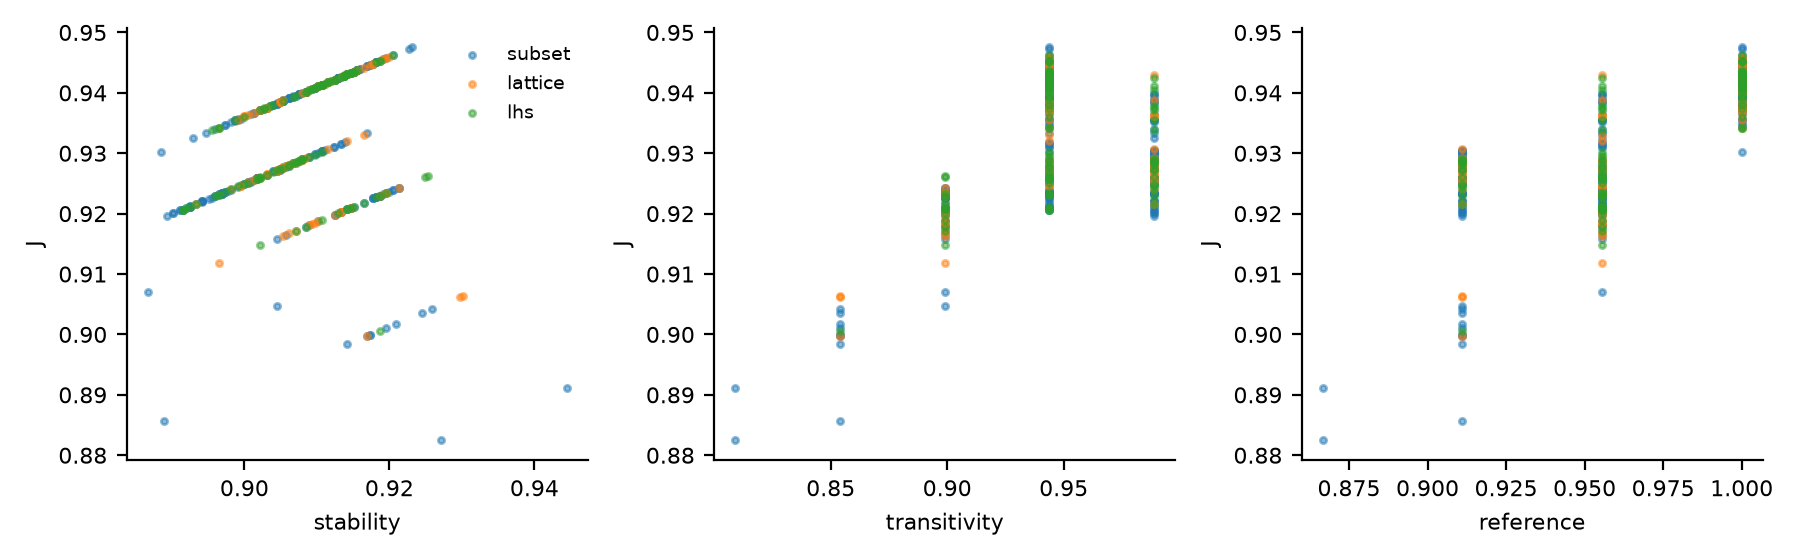
\includegraphics[width=0.9\textwidth]{fig_j_terms.png}\caption{Objective $J$ against each of its three terms (stability, transitivity, reference) for every candidate mix.}\label{figall:fig_j_terms}\end{figure}
\begin{figure}[htbp]\centering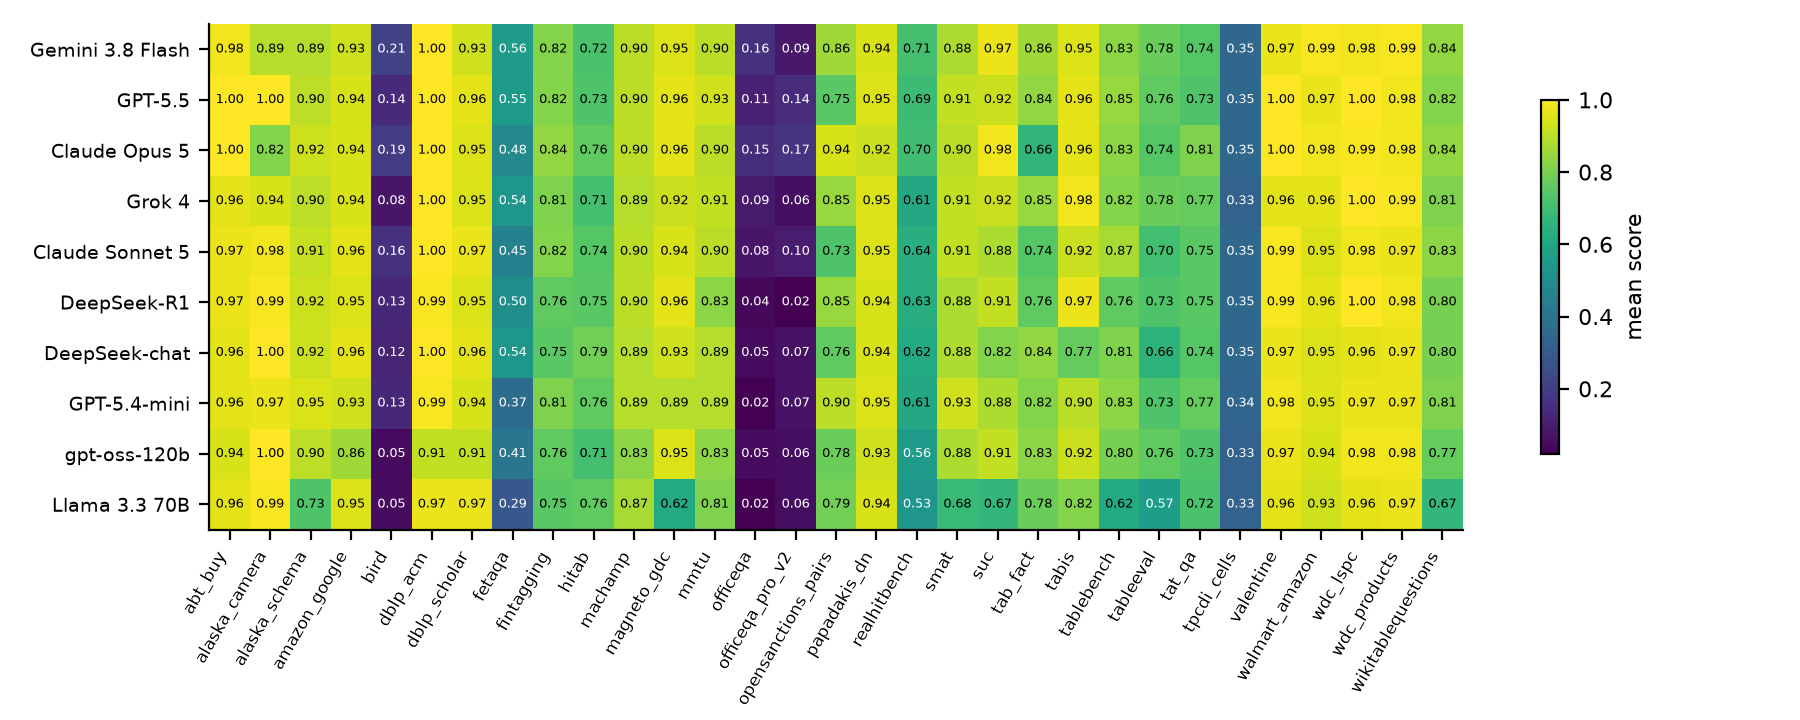
\includegraphics[width=0.9\textwidth]{fig_model_dataset_heatmap.png}\caption{Mean score per model and dataset under the headline rule.}\label{figall:fig_model_dataset_heatmap}\end{figure}
\begin{figure}[htbp]\centering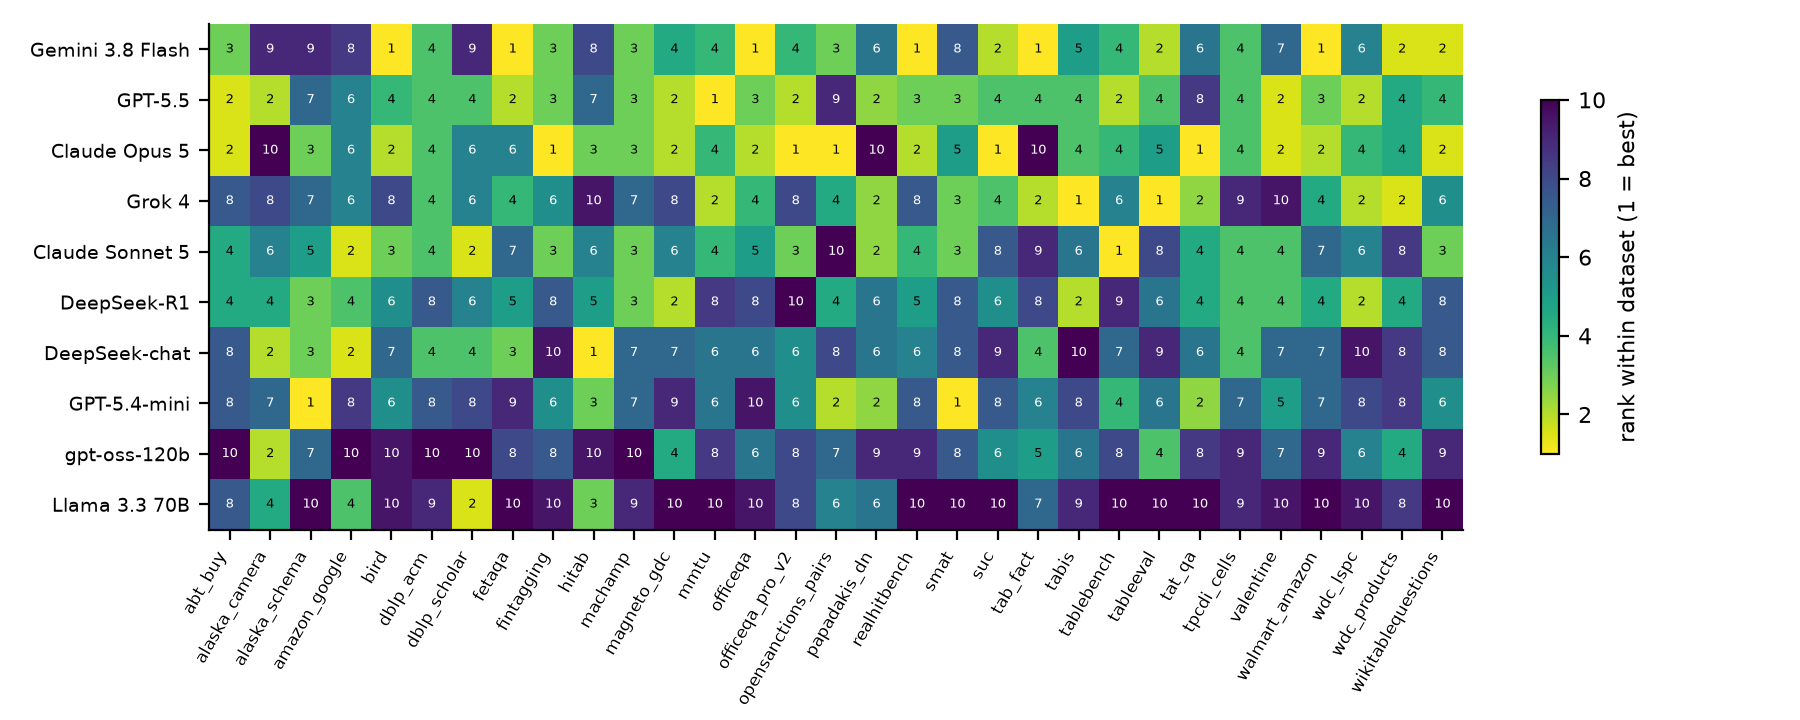
\includegraphics[width=0.9\textwidth]{fig_model_dataset_ranks.png}\caption{Rank per model and dataset under the headline rule.}\label{figall:fig_model_dataset_ranks}\end{figure}
\begin{figure}[htbp]\centering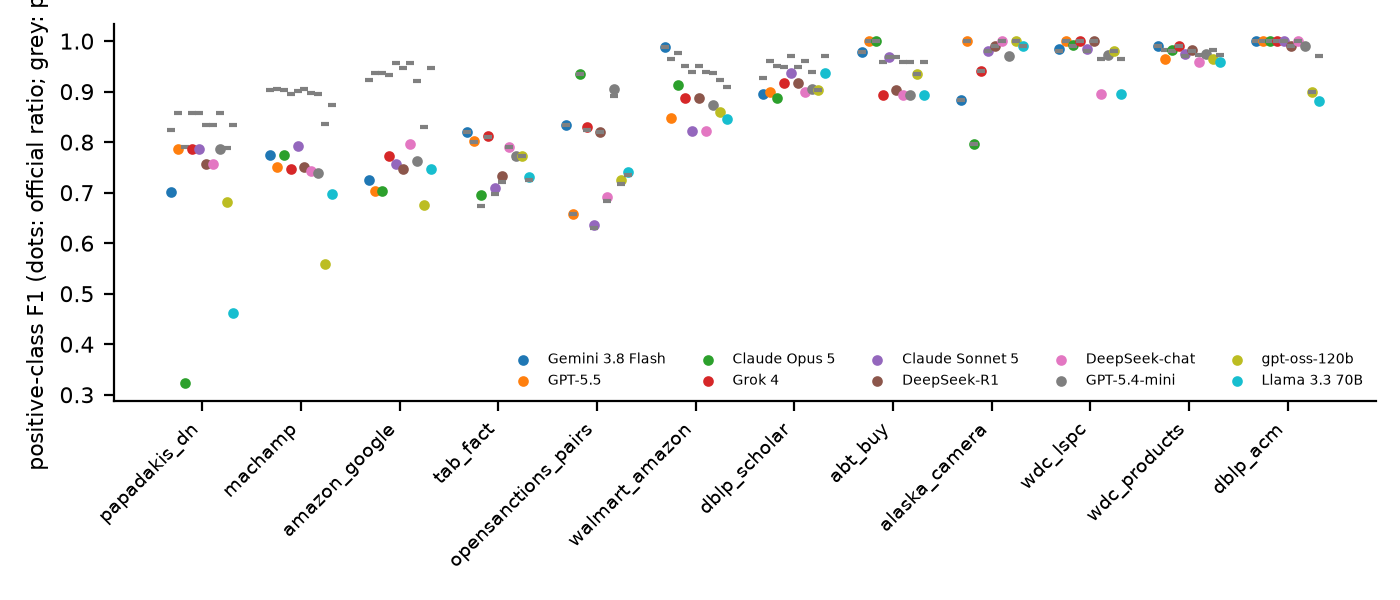
\includegraphics[width=0.9\textwidth]{fig_official_f1_models.png}\caption{Positive-class F1 on the balanced pool (grey) and at the official match ratio (coloured) per model and matching dataset.}\label{figall:fig_official_f1_models}\end{figure}
\begin{figure}[htbp]\centering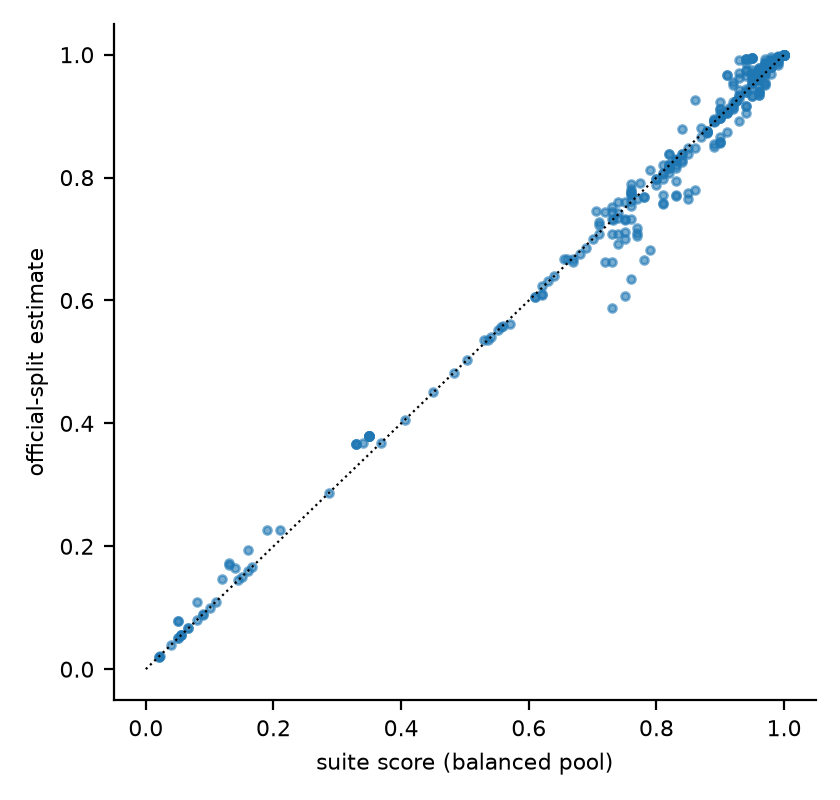
\includegraphics[width=0.9\textwidth]{fig_official_scatter.png}\caption{Suite score against post-stratified official-split estimate for every (dataset, model) pair under the headline rule.}\label{figall:fig_official_scatter}\end{figure}
\begin{figure}[htbp]\centering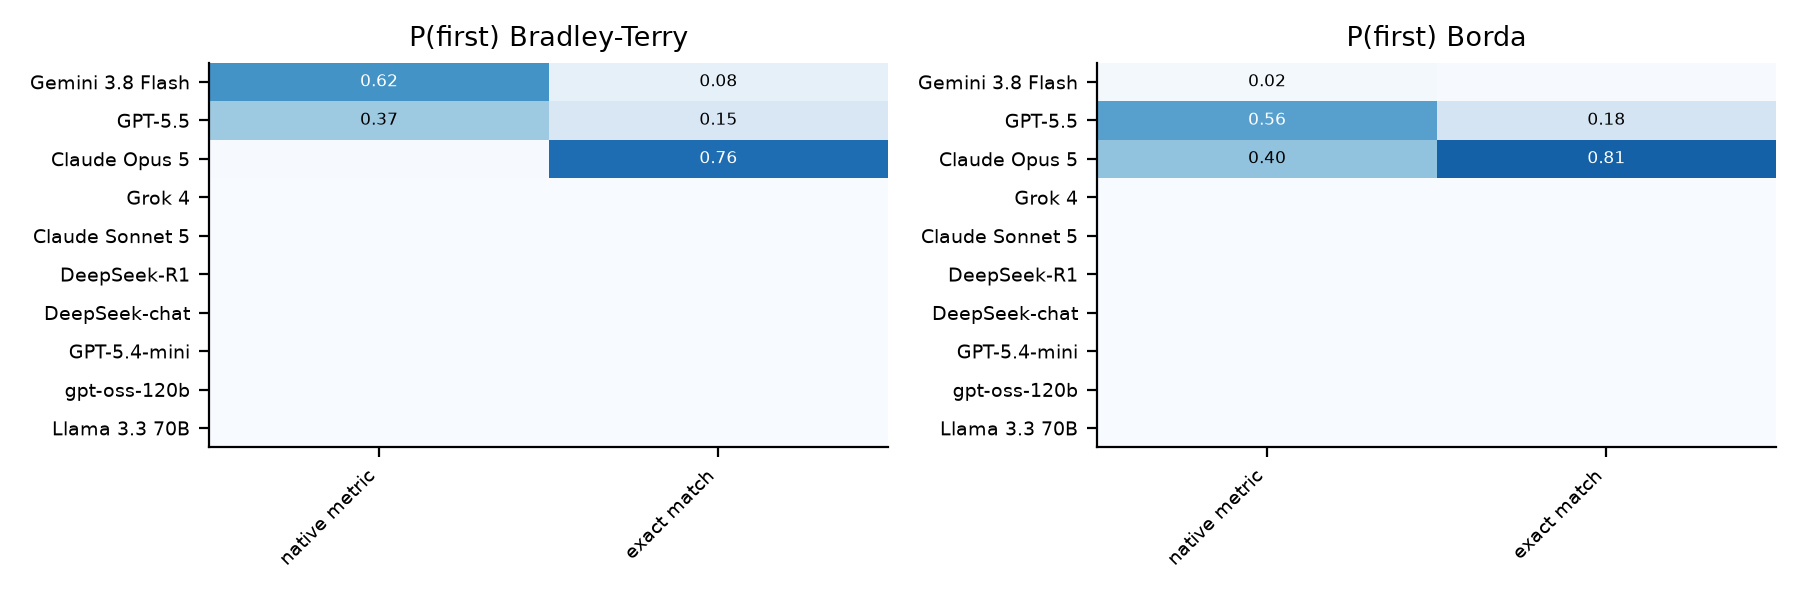
\includegraphics[width=0.9\textwidth]{fig_p_first.png}\caption{Bootstrap probability of first place under every rule, by pooling method.}\label{figall:fig_p_first}\end{figure}
\begin{figure}[htbp]\centering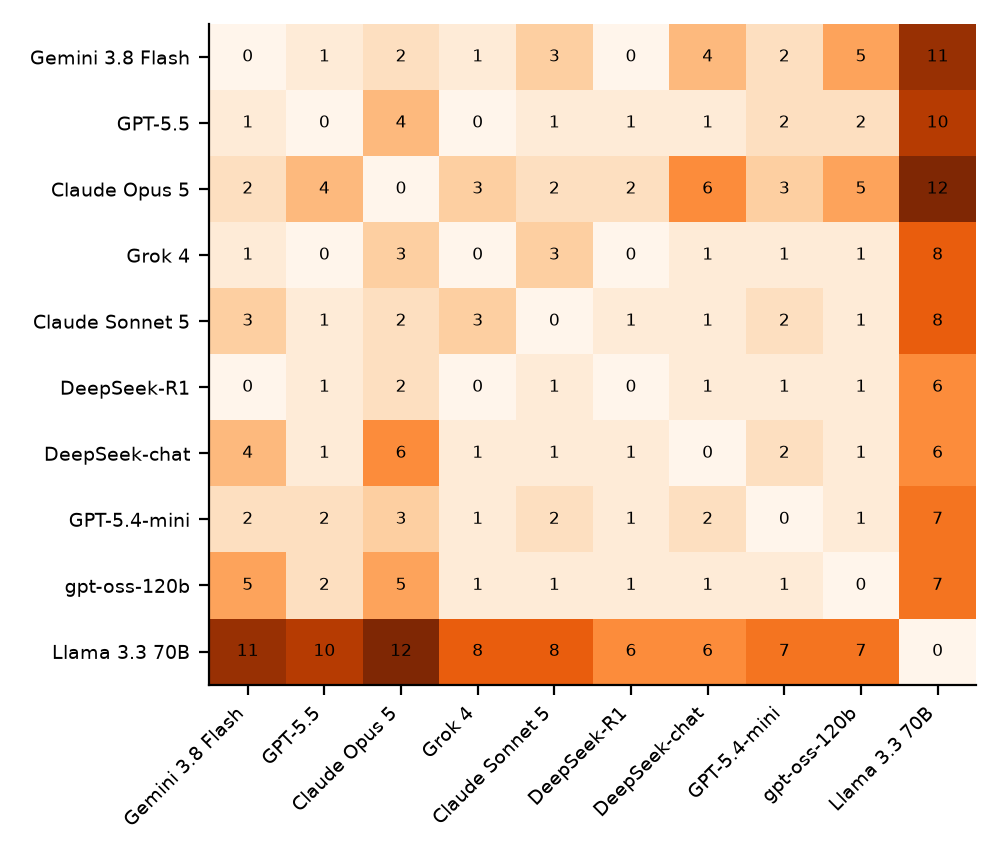
\includegraphics[width=0.9\textwidth]{fig_pairwise_significance.png}\caption{Number of datasets (of 31) in which the per-item paired test separates each pair of models under the headline rule (Holm within dataset).}\label{figall:fig_pairwise_significance}\end{figure}
\begin{figure}[htbp]\centering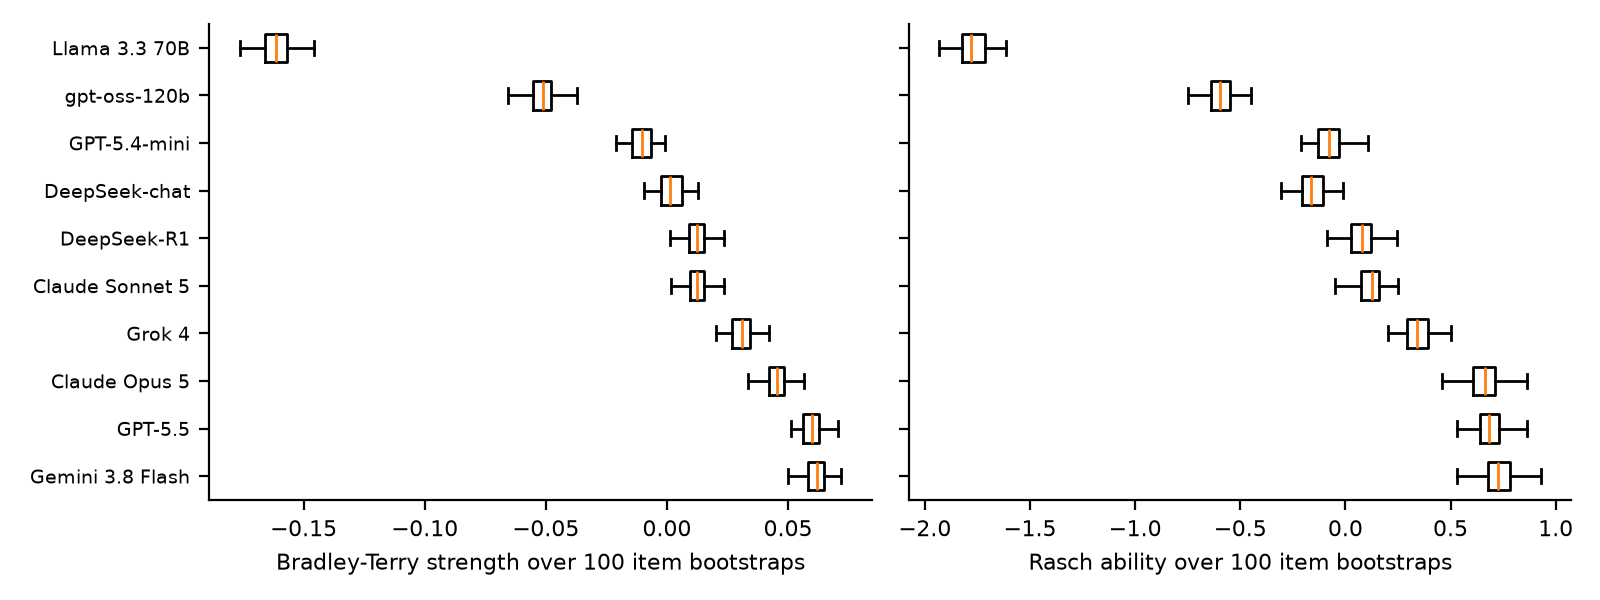
\includegraphics[width=0.9\textwidth]{fig_parameter_bootstrap.png}\caption{Bootstrap distributions of the Bradley--Terry strengths and Rasch abilities (100 item resamples).}\label{figall:fig_parameter_bootstrap}\end{figure}
\begin{figure}[htbp]\centering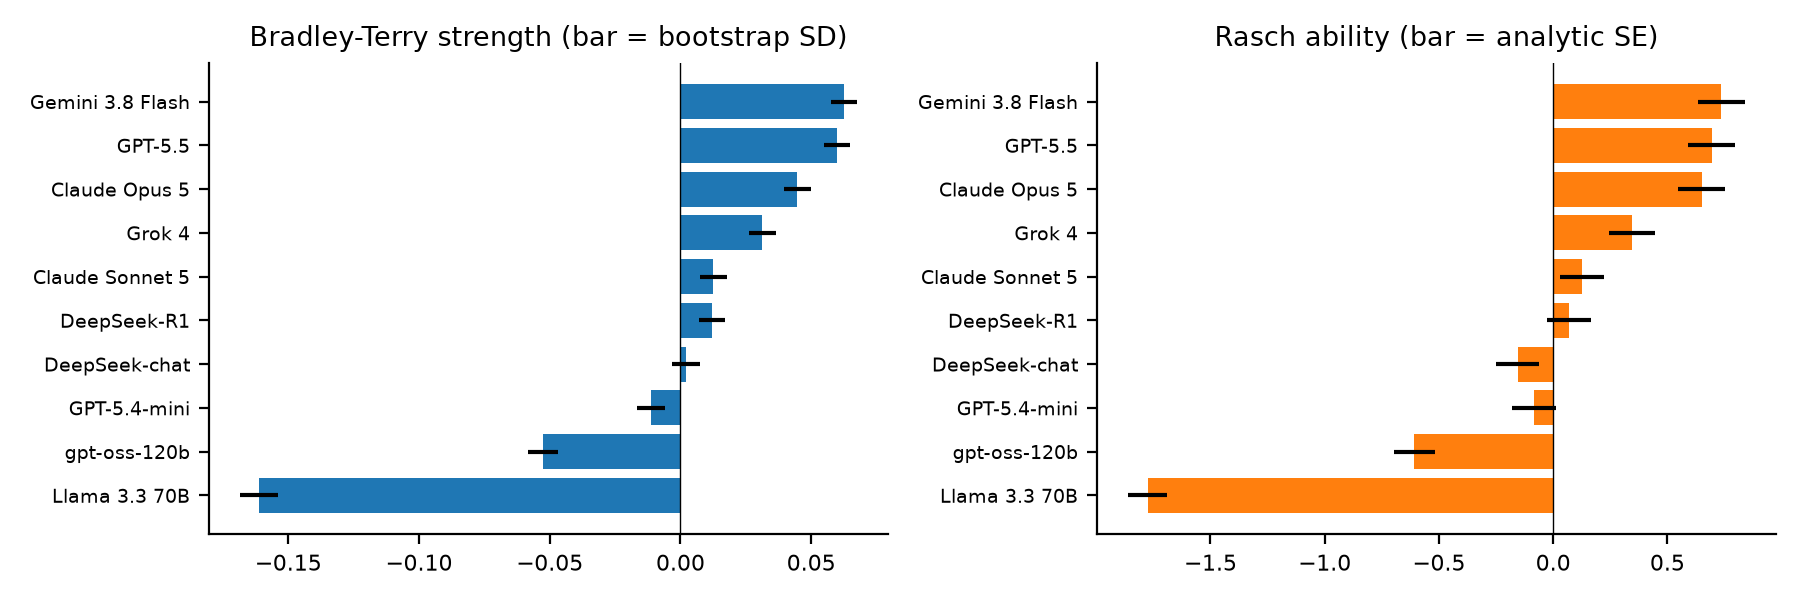
\includegraphics[width=0.9\textwidth]{fig_parameters.png}\caption{Fitted Bradley--Terry strengths and Rasch abilities with their uncertainty.}\label{figall:fig_parameters}\end{figure}
\begin{figure}[htbp]\centering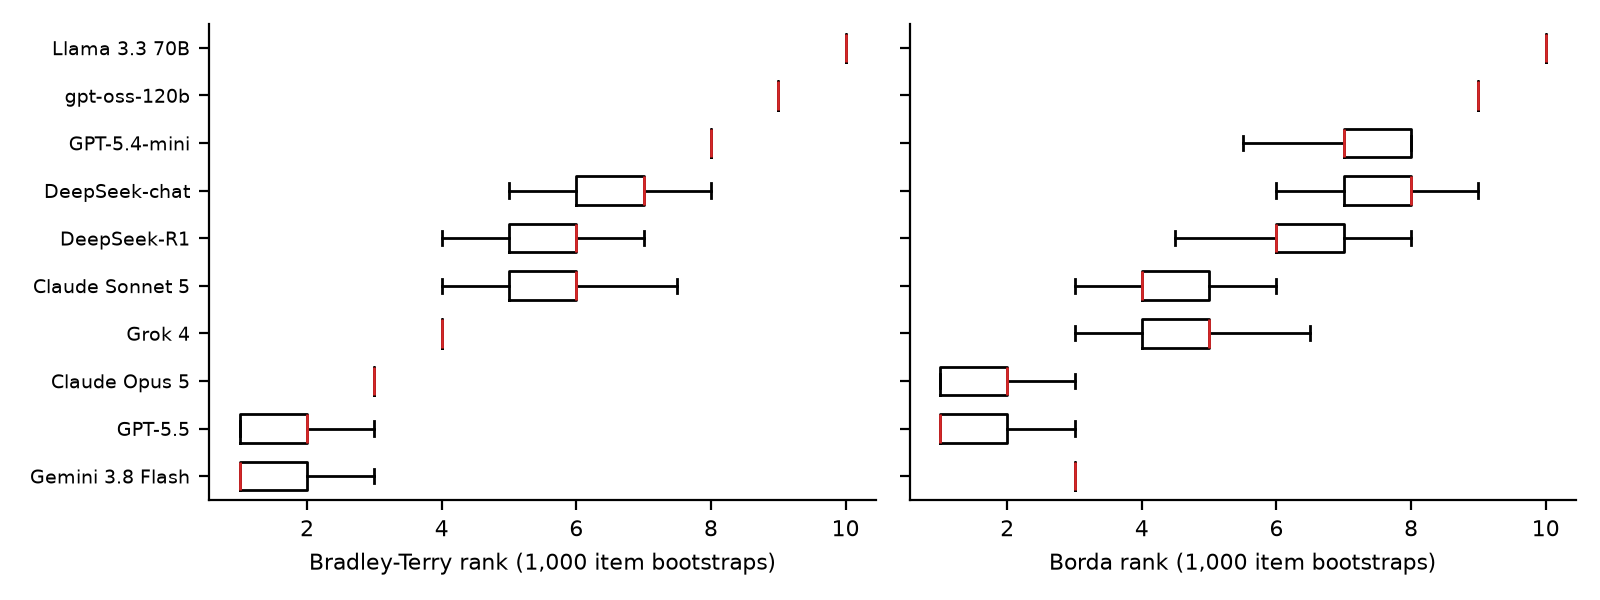
\includegraphics[width=0.9\textwidth]{fig_rank_bootstrap.png}\caption{Bootstrap distribution of each model's rank under the headline rule (native metric).}\label{figall:fig_rank_bootstrap}\end{figure}
\begin{figure}[htbp]\centering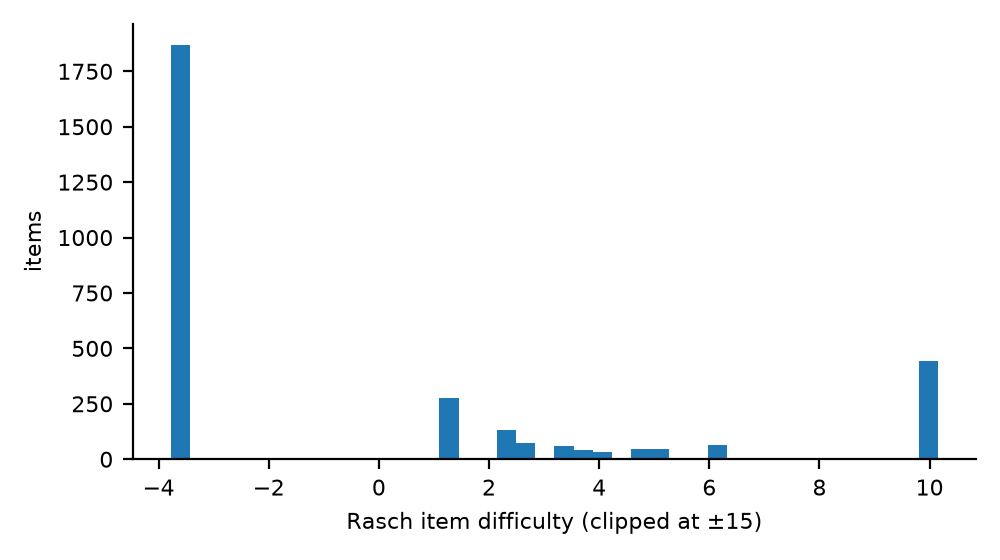
\includegraphics[width=0.9\textwidth]{fig_rasch_items.png}\caption{Distribution of Rasch item difficulties over the 3,083 items.}\label{figall:fig_rasch_items}\end{figure}
\begin{figure}[htbp]\centering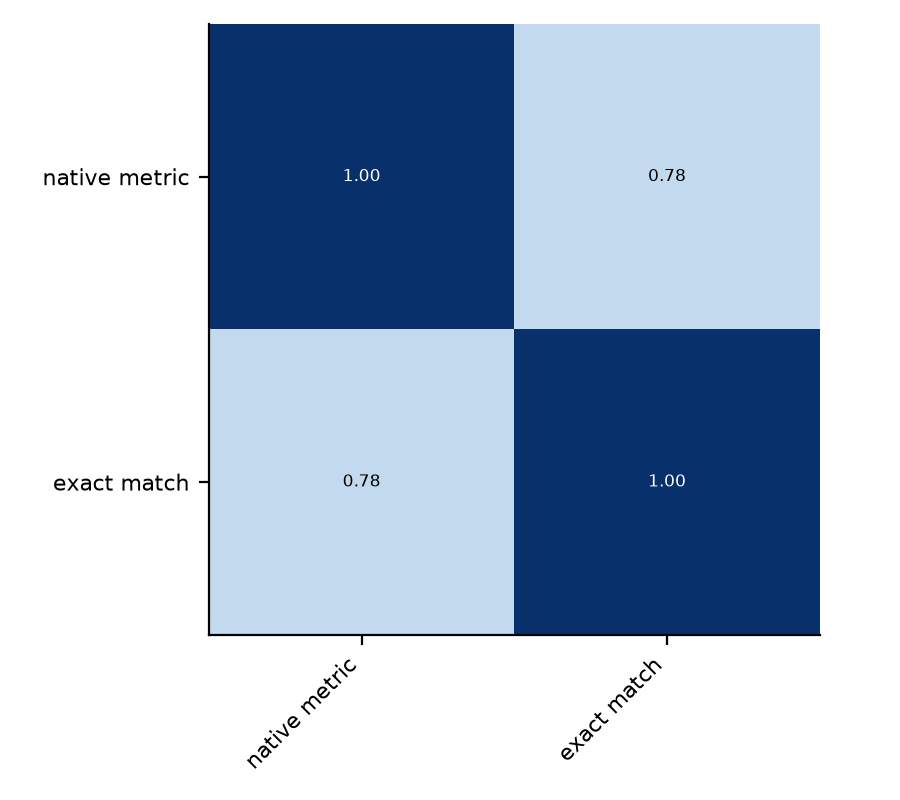
\includegraphics[width=0.9\textwidth]{fig_rule_agreement.png}\caption{Kendall $\tau$ between the Bradley--Terry rankings of each pair of rules.}\label{figall:fig_rule_agreement}\end{figure}
\begin{figure}[htbp]\centering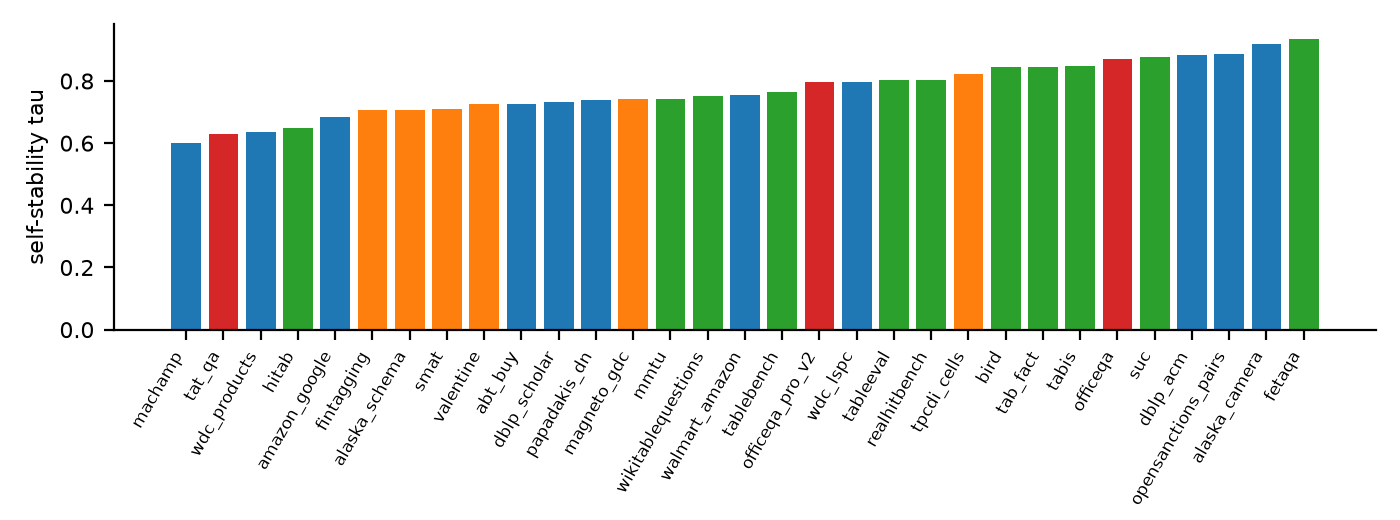
\includegraphics[width=0.9\textwidth]{fig_self_stability.png}\caption{Self-stability of each dataset's model ranking (Kendall $\tau$ between bootstrap halves).}\label{figall:fig_self_stability}\end{figure}
\begin{figure}[htbp]\centering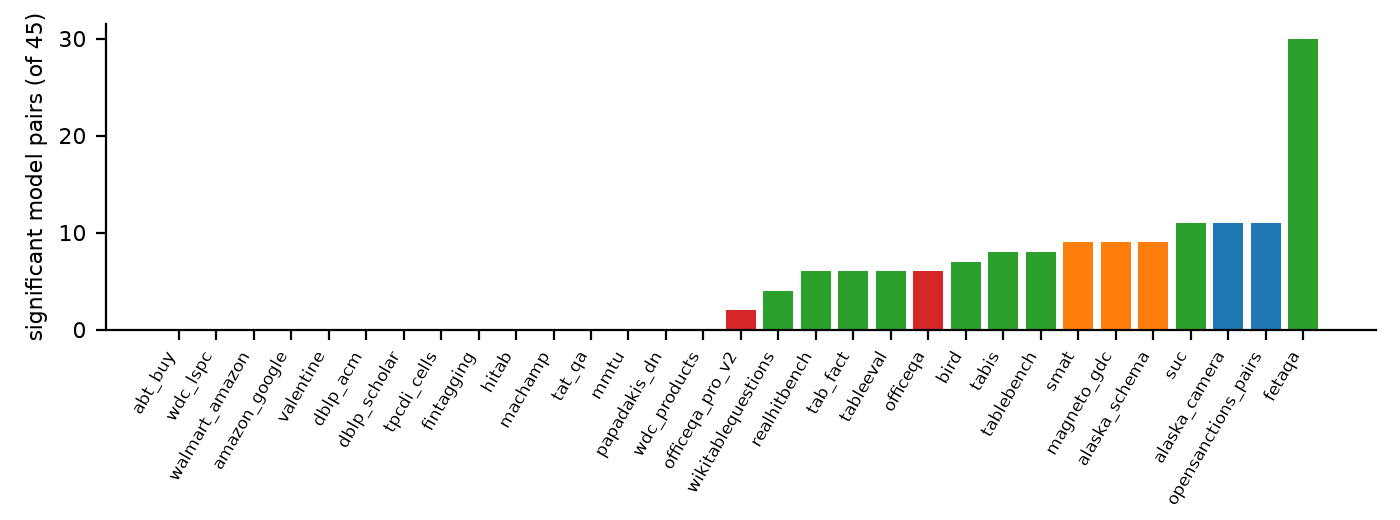
\includegraphics[width=0.9\textwidth]{fig_significant_pairs_per_dataset.png}\caption{How many of the 45 model pairs each dataset separates at the item level under the headline rule (colour = family).}\label{figall:fig_significant_pairs_per_dataset}\end{figure}
\begin{figure}[htbp]\centering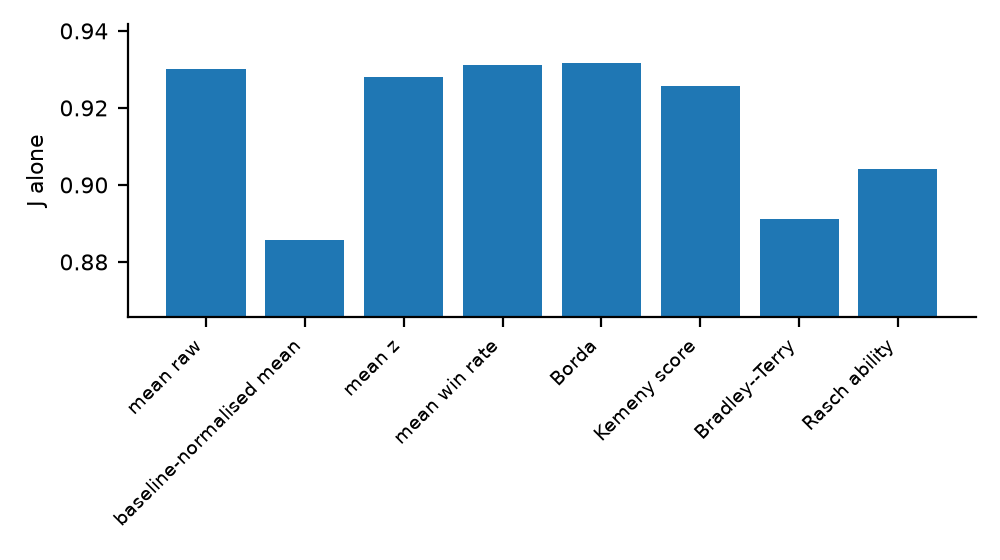
\includegraphics[width=0.9\textwidth]{fig_single_view_j.png}\caption{Objective $J$ of each view used alone.}\label{figall:fig_single_view_j}\end{figure}
\begin{figure}[htbp]\centering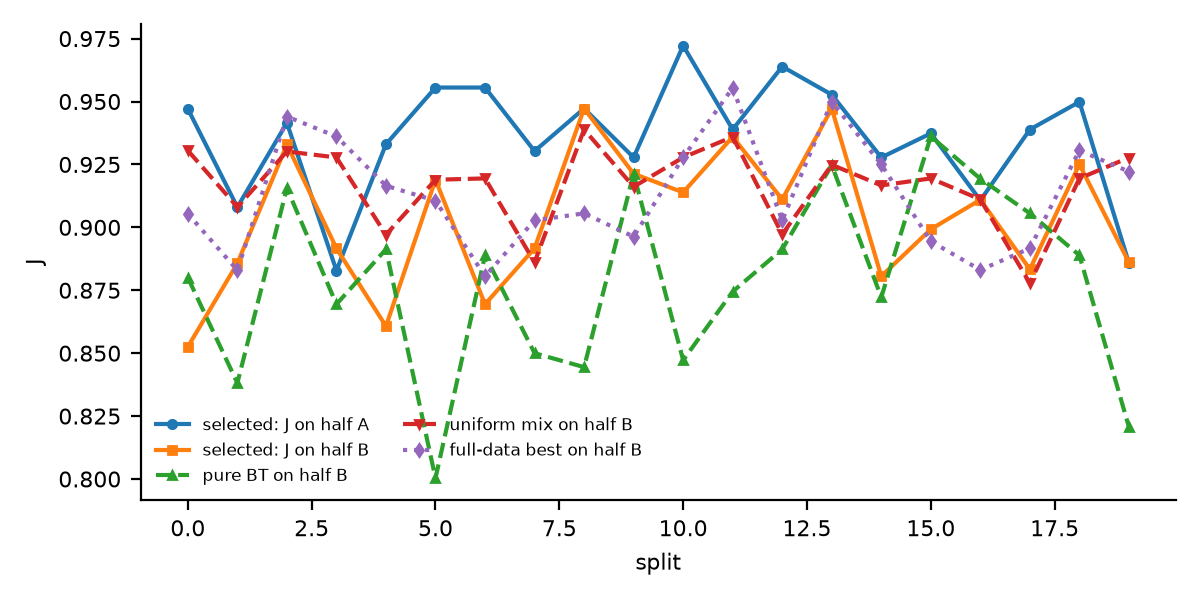
\includegraphics[width=0.9\textwidth]{fig_split_half.png}\caption{Split-half honesty check: the mix selected on half A scored on both halves, against pure Bradley--Terry, the uniform mix and the full-data best on half B.}\label{figall:fig_split_half}\end{figure}
\begin{figure}[htbp]\centering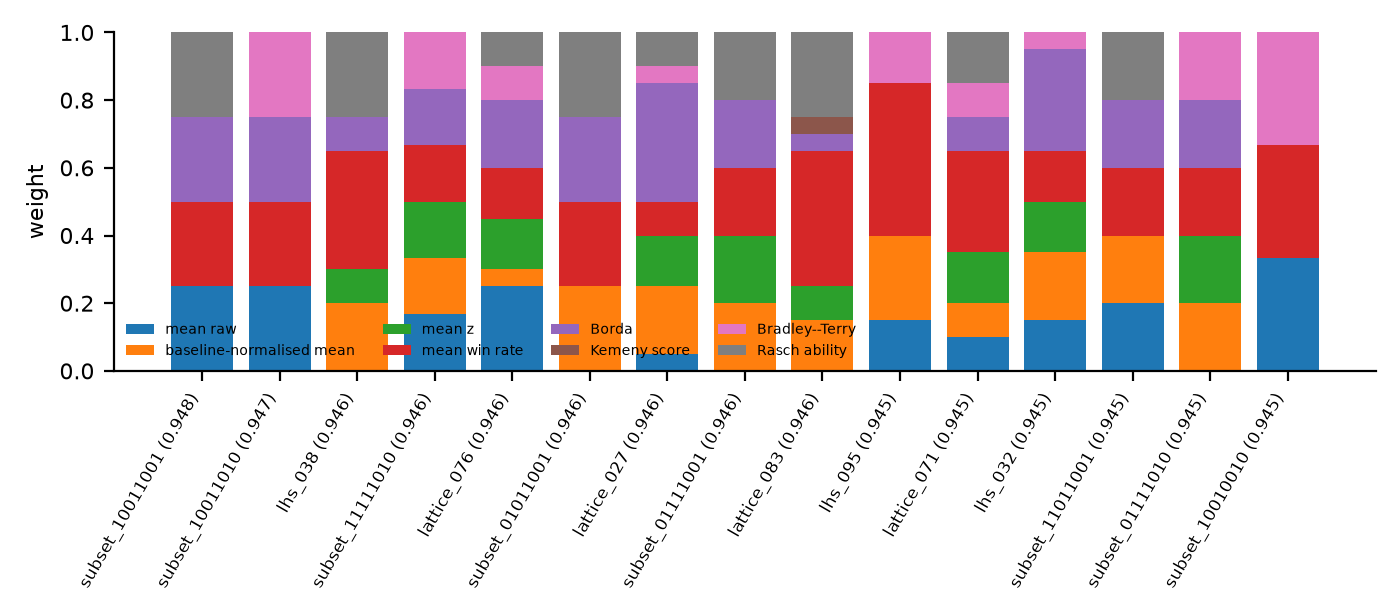
\includegraphics[width=0.9\textwidth]{fig_top_mix_weights.png}\caption{View weights of the fifteen best candidate mixes (label and $J$ on the axis).}\label{figall:fig_top_mix_weights}\end{figure}
\begin{figure}[htbp]\centering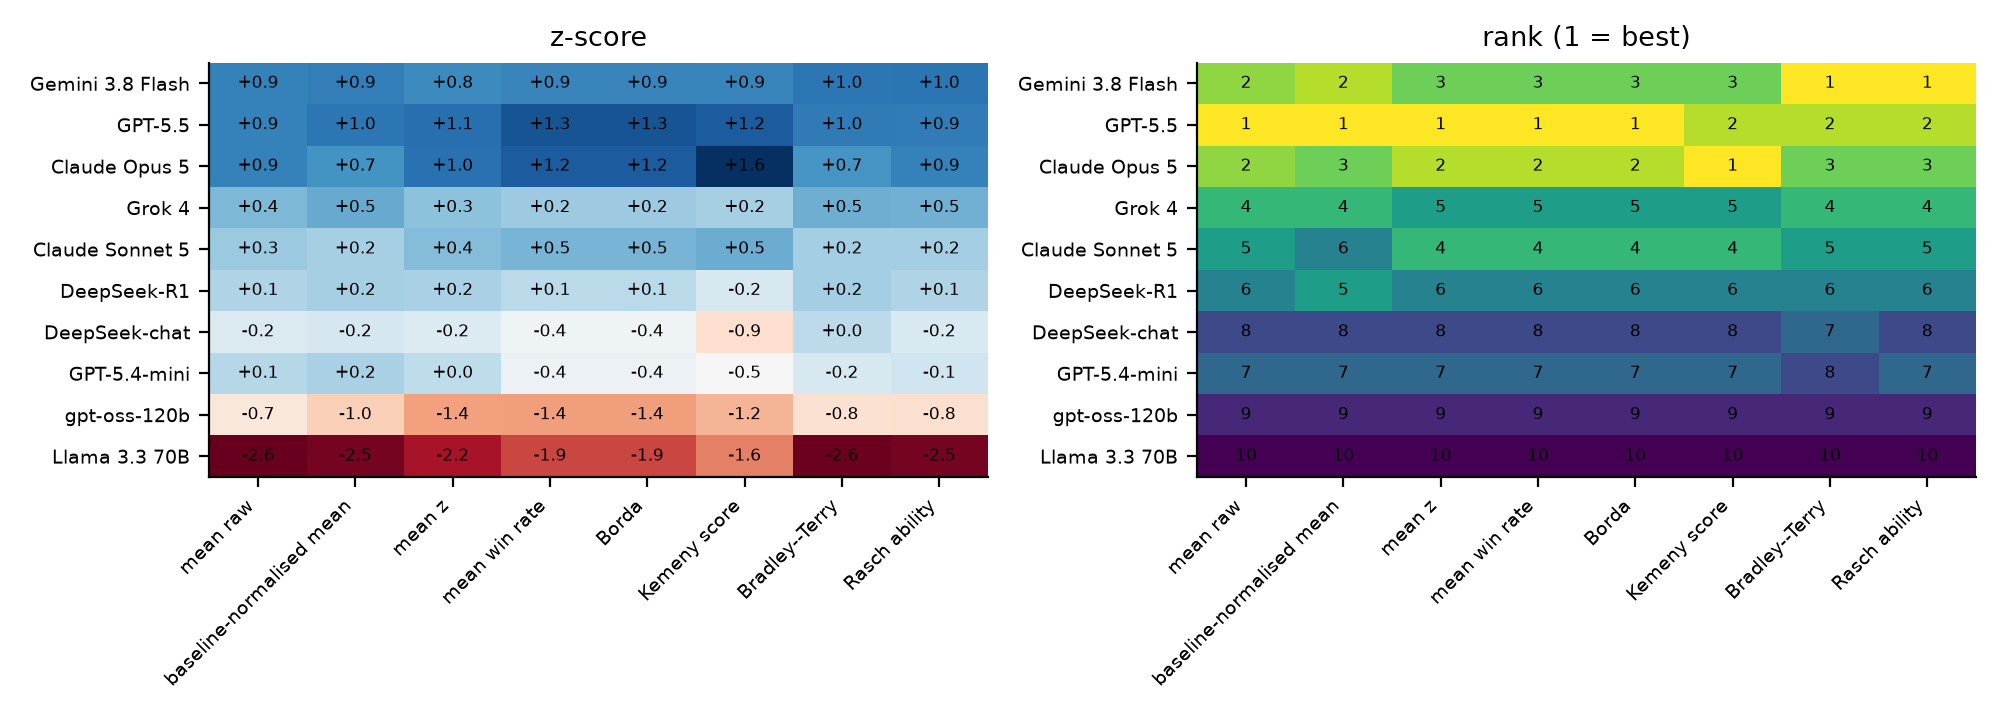
\includegraphics[width=0.9\textwidth]{fig_view_matrix.png}\caption{Each view's z-score (left) and rank (right) per model on native-metric scores.}\label{figall:fig_view_matrix}\end{figure}
\begin{figure}[htbp]\centering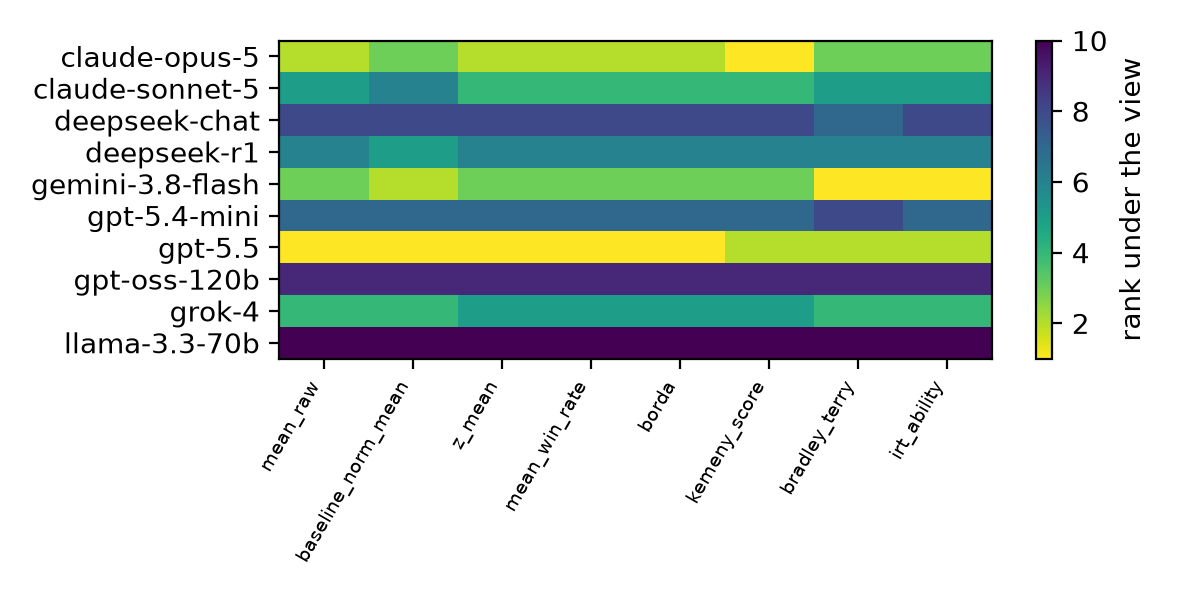
\includegraphics[width=0.9\textwidth]{fig_views.png}\caption{The eight single views: z-scored value per model.}\label{figall:fig_views}\end{figure}
\clearpage
\section{All tables}
Every saved table, one file each under \texttt{tables/}; include any in the main text with \texttt{\textbackslash input}.
\begin{table}[htbp]
\centering\scriptsize
\caption{Best equal-weight subset for each subset size.}
\label{tab:best_subset_per_size}
\setlength{\tabcolsep}{3pt}
\begin{tabular}{lp{0.381\linewidth}rrp{0.305\linewidth}r}
\toprule
n\_\allowbreak{}views & label & J & stability & transitivity & reference \\
\midrule
1 & subset\_\allowbreak{}00001000 & 0.932 & 0.914 & 0.944 & 0.956 \\
2 & subset\_\allowbreak{}00010001 & 0.944 & 0.916 & 0.944 & 1.000 \\
3 & subset\_\allowbreak{}10010010 & 0.945 & 0.918 & 0.944 & 1.000 \\
4 & subset\_\allowbreak{}10011001 & 0.948 & 0.923 & 0.944 & 1.000 \\
5 & subset\_\allowbreak{}01111001 & 0.946 & 0.919 & 0.944 & 1.000 \\
6 & subset\_\allowbreak{}11111010 & 0.946 & 0.920 & 0.944 & 1.000 \\
7 & subset\_\allowbreak{}11111011 & 0.944 & 0.915 & 0.944 & 1.000 \\
8 & subset\_\allowbreak{}11111111 & 0.941 & 0.911 & 0.944 & 1.000 \\
\bottomrule
\end{tabular}
\end{table}

\clearpage
\begin{table}[htbp]
\centering\tiny
\caption{Sampled designs of 100 mixes: coverage diagnostics.}
\label{tab:designs}
\setlength{\tabcolsep}{3pt}
\begin{tabular}{lrrp{0.099\linewidth}p{0.099\linewidth}p{0.146\linewidth}p{0.205\linewidth}p{0.159\linewidth}}
\toprule
design & n & K & min\_\allowbreak{}pairwise\_\allowbreak{}L1 & mean\_\allowbreak{}nearest\_\allowbreak{}L1 & centred\_\allowbreak{}L2\_\allowbreak{}discrepancy & mean\_\allowbreak{}distinct\_\allowbreak{}values\_\allowbreak{}per\_\allowbreak{}weight & share\_\allowbreak{}with\_\allowbreak{}a\_\allowbreak{}zero\_\allowbreak{}weight \\
\midrule
lattice & 100 & 8 & 0.200 & 0.401 & 1.993 & 11.625 & 0.930 \\
lhs & 100 & 8 & 0.100 & 0.366 & 2.071 & 10.500 & 0.760 \\
\bottomrule
\end{tabular}
\end{table}

\clearpage
\begin{landscape}
\tiny
\setlength{\tabcolsep}{3pt}
\begin{longtable}{p{0.147\linewidth}p{0.073\linewidth}p{0.073\linewidth}p{0.073\linewidth}p{0.073\linewidth}p{0.073\linewidth}p{0.073\linewidth}p{0.073\linewidth}p{0.073\linewidth}p{0.073\linewidth}p{0.073\linewidth}}
\caption{Dataset diagnostics under the headline rule.}\label{tab:diagnostics}\\
\toprule
dataset & family & mean\_\allowbreak{}score & spread\_\allowbreak{}across\_\allowbreak{}models & floor & ceiling & share\_\allowbreak{}constant\_\allowbreak{}bootstrap\_\allowbreak{}rankings & ranking\_\allowbreak{}self\_\allowbreak{}stability\_\allowbreak{}tau & tau\_\allowbreak{}to\_\allowbreak{}others\_\allowbreak{}mean & n\_\allowbreak{}items & exclude\_\allowbreak{}from\_\allowbreak{}objective \\
\midrule
abt\_\allowbreak{}buy & EM & 0.970 & 0.060 & no & no & 0.000 & 0.726 & 0.369 & 100 & no \\
alaska\_\allowbreak{}camera & EM & 0.958 & 0.180 & no & no & 0.000 & 0.919 & -0.219 & 100 & no \\
alaska\_\allowbreak{}schema & SM & 0.897 & 0.215 & no & no & 0.000 & 0.707 & 0.055 & 93 & no \\
amazon\_\allowbreak{}google & EM & 0.936 & 0.100 & no & no & 0.000 & 0.684 & -0.018 & 100 & no \\
bird & TQA & 0.126 & 0.160 & no & no & 0.000 & 0.844 & 0.364 & 100 & no \\
dblp\_\allowbreak{}acm & EM & 0.986 & 0.090 & no & no & 0.000 & 0.884 & 0.358 & 100 & no \\
dblp\_\allowbreak{}scholar & EM & 0.949 & 0.060 & no & no & 0.000 & 0.733 & -0.025 & 100 & no \\
fetaqa & TQA & 0.468 & 0.270 & no & no & 0.000 & 0.937 & 0.282 & 100 & no \\
fintagging & SM & 0.794 & 0.090 & no & no & 0.000 & 0.707 & 0.376 & 100 & no \\
hitab & TQA & 0.743 & 0.080 & no & no & 0.000 & 0.647 & -0.091 & 100 & no \\
machamp & EM & 0.887 & 0.070 & no & no & 0.000 & 0.600 & 0.396 & 100 & no \\
magneto\_\allowbreak{}gdc & SM & 0.908 & 0.340 & no & no & 0.000 & 0.741 & 0.265 & 100 & no \\
mmtu & TQA & 0.879 & 0.120 & no & no & 0.000 & 0.743 & 0.362 & 100 & no \\
officeqa & FIN & 0.077 & 0.140 & no & no & 0.000 & 0.870 & 0.325 & 100 & no \\
officeqa\_\allowbreak{}pro\_\allowbreak{}v2 & FIN & 0.082 & 0.144 & no & no & 0.000 & 0.795 & 0.303 & 90 & no \\
opensanctions\_\allowbreak{}pairs & EM & 0.821 & 0.210 & no & no & 0.000 & 0.888 & 0.025 & 100 & no \\
papadakis\_\allowbreak{}dn & EM & 0.941 & 0.030 & no & no & 0.002 & 0.739 & 0.074 & 100 & no \\
realhitbench & TQA & 0.630 & 0.180 & no & no & 0.000 & 0.803 & 0.385 & 100 & no \\
smat & SM & 0.876 & 0.250 & no & no & 0.000 & 0.711 & 0.196 & 100 & no \\
suc & TQA & 0.886 & 0.310 & no & no & 0.000 & 0.879 & 0.322 & 100 & no \\
tab\_\allowbreak{}fact & TQA & 0.798 & 0.200 & no & no & 0.000 & 0.845 & -0.002 & 100 & no \\
tabis & TQA & 0.915 & 0.210 & no & no & 0.000 & 0.849 & 0.239 & 100 & no \\
tablebench & TQA & 0.802 & 0.250 & no & no & 0.000 & 0.766 & 0.316 & 100 & no \\
tableeval & TQA & 0.721 & 0.210 & no & no & 0.000 & 0.803 & 0.192 & 100 & no \\
tat\_\allowbreak{}qa & FIN & 0.751 & 0.090 & no & no & 0.000 & 0.628 & 0.195 & 100 & no \\
tpcdi\_\allowbreak{}cells & SM & 0.343 & 0.020 & no & no & 0.058 & 0.821 & 0.329 & 100 & no \\
valentine & SM & 0.979 & 0.040 & no & yes & 0.000 & 0.725 & 0.296 & 100 & yes \\
walmart\_\allowbreak{}amazon & EM & 0.958 & 0.060 & no & no & 0.000 & 0.755 & 0.386 & 100 & no \\
wdc\_\allowbreak{}lspc & EM & 0.982 & 0.040 & no & yes & 0.004 & 0.796 & 0.268 & 100 & yes \\
wdc\_\allowbreak{}products & EM & 0.978 & 0.020 & no & yes & 0.006 & 0.637 & 0.188 & 100 & yes \\
wikitablequestions & TQA & 0.799 & 0.170 & no & no & 0.000 & 0.751 & 0.393 & 100 & no \\
\bottomrule
\end{longtable}
\normalsize
\end{landscape}

\clearpage
\begin{landscape}
\begin{table}[htbp]
\centering\tiny
\caption{Full leaderboard under rule exact match; weights: --.}
\label{tab:leaderboard_em_only}
\setlength{\tabcolsep}{3pt}
\resizebox{\linewidth}{!}{%
\begin{tabular}{lrrrrrrrrrrrrrrrr}
\toprule
model & bt\_\allowbreak{}strength & bt\_\allowbreak{}se\_\allowbreak{}vs\_\allowbreak{}ref & rank\_\allowbreak{}bt & bt\_\allowbreak{}rank\_\allowbreak{}lo95 & bt\_\allowbreak{}rank\_\allowbreak{}hi95 & p\_\allowbreak{}first\_\allowbreak{}bt & rank\_\allowbreak{}borda & borda\_\allowbreak{}rank\_\allowbreak{}lo95 & borda\_\allowbreak{}rank\_\allowbreak{}hi95 & p\_\allowbreak{}first\_\allowbreak{}borda & rank\_\allowbreak{}kemeny & rank\_\allowbreak{}copeland & rank\_\allowbreak{}mean\_\allowbreak{}z & rank\_\allowbreak{}rrf & rank\_\allowbreak{}family\_\allowbreak{}balanced\_\allowbreak{}z & mean\_\allowbreak{}score \\
\midrule
Claude Opus 5 & 0.047 & 0.000 & 1.000 & 1.000 & 3.000 & 0.764 & 1.000 & 1.000 & 2.000 & 0.812 & 1.000 & 1.000 & 1.000 & 1.000 & 1.000 & 0.768 \\
GPT-5.5 & 0.039 & 0.016 & 2.000 & 1.000 & 3.000 & 0.152 & 2.000 & 1.000 & 3.000 & 0.177 & 2.000 & 2.000 & 2.000 & 2.000 & 2.000 & 0.764 \\
Gemini 3.8 Flash & 0.037 & 0.016 & 3.000 & 1.000 & 3.000 & 0.084 & 3.000 & 2.000 & 5.000 & 0.004 & 3.000 & 3.000 & 3.000 & 3.000 & 3.000 & 0.763 \\
Grok 4 & 0.020 & 0.016 & 4.000 & 4.000 & 6.000 & 0.000 & 5.000 & 3.000 & 6.012 & 0.000 & 5.000 & 5.000 & 5.000 & 5.000 & 5.000 & 0.754 \\
Claude Sonnet 5 & 0.013 & 0.016 & 5.000 & 4.000 & 7.000 & 0.000 & 4.000 & 3.000 & 6.000 & 0.000 & 4.000 & 4.000 & 4.000 & 4.000 & 4.000 & 0.751 \\
GPT-5.4-mini & 0.010 & 0.016 & 6.000 & 4.000 & 7.000 & 0.000 & 8.000 & 6.000 & 8.000 & 0.000 & 7.000 & 7.000 & 7.000 & 8.000 & 8.000 & 0.749 \\
DeepSeek-R1 & 0.008 & 0.016 & 7.000 & 5.000 & 7.000 & 0.000 & 6.000 & 4.000 & 8.000 & 0.000 & 6.000 & 6.000 & 6.000 & 6.000 & 6.000 & 0.748 \\
DeepSeek-chat & -0.014 & 0.016 & 8.000 & 8.000 & 9.000 & 0.000 & 7.000 & 6.000 & 8.000 & 0.000 & 8.000 & 8.000 & 8.000 & 7.000 & 7.000 & 0.737 \\
gpt-oss-120b & -0.033 & 0.016 & 9.000 & 8.000 & 9.000 & 0.000 & 9.000 & 9.000 & 9.000 & 0.000 & 9.000 & 9.000 & 9.000 & 9.000 & 9.000 & 0.728 \\
Llama 3.3 70B & -0.128 & 0.016 & 10.000 & 10.000 & 10.000 & 0.000 & 10.000 & 10.000 & 10.000 & 0.000 & 10.000 & 10.000 & 10.000 & 10.000 & 10.000 & 0.680 \\
\bottomrule
\end{tabular}
}
\end{table}
\end{landscape}

\clearpage
\begin{table}[htbp]
\centering\tiny
\caption{Leaderboard under the headline rule (native metric).}
\label{tab:leaderboard_headline}
\setlength{\tabcolsep}{3pt}
\begin{tabular}{lp{0.256\linewidth}p{0.176\linewidth}rrrp{0.176\linewidth}r}
\toprule
rank & model & BT strength & SE & Borda rank & Borda 95\% & P(first) BT & mean score \\
\midrule
1 & Gemini 3.8 Flash & 0.063 & 0.016 & 3 & [2, 4] & 0.620 & 0.792 \\
2 & GPT-5.5 & 0.060 & 0.016 & 1 & [1, 3] & 0.370 & 0.793 \\
3 & Claude Opus 5 & 0.045 & 0.000 & 2 & [1, 3] & 0.000 & 0.792 \\
4 & Grok 4 & 0.031 & 0.016 & 5 & [3, 6] & 0.000 & 0.780 \\
5 & Claude Sonnet 5 & 0.012 & 0.016 & 4 & [3, 6] & 0.000 & 0.776 \\
6 & DeepSeek-R1 & 0.012 & 0.016 & 6 & [4, 8] & 0.000 & 0.772 \\
7 & DeepSeek-chat & 0.002 & 0.016 & 8 & [6, 8] & 0.000 & 0.763 \\
8 & GPT-5.4-mini & -0.011 & 0.016 & 7 & [6, 8] & 0.000 & 0.771 \\
9 & gpt-oss-120b & -0.053 & 0.016 & 9 & [9, 9] & 0.000 & 0.750 \\
10 & Llama 3.3 70B & -0.161 & 0.016 & 10 & [10, 10] & 0.000 & 0.701 \\
\bottomrule
\end{tabular}
\end{table}

\clearpage
\begin{landscape}
\begin{table}[htbp]
\centering\tiny
\caption{Full leaderboard under rule native metric; weights: --.}
\label{tab:leaderboard_native}
\setlength{\tabcolsep}{3pt}
\resizebox{\linewidth}{!}{%
\begin{tabular}{lrrrrrrrrrrrrrrrr}
\toprule
model & bt\_\allowbreak{}strength & bt\_\allowbreak{}se\_\allowbreak{}vs\_\allowbreak{}ref & rank\_\allowbreak{}bt & bt\_\allowbreak{}rank\_\allowbreak{}lo95 & bt\_\allowbreak{}rank\_\allowbreak{}hi95 & p\_\allowbreak{}first\_\allowbreak{}bt & rank\_\allowbreak{}borda & borda\_\allowbreak{}rank\_\allowbreak{}lo95 & borda\_\allowbreak{}rank\_\allowbreak{}hi95 & p\_\allowbreak{}first\_\allowbreak{}borda & rank\_\allowbreak{}kemeny & rank\_\allowbreak{}copeland & rank\_\allowbreak{}mean\_\allowbreak{}z & rank\_\allowbreak{}rrf & rank\_\allowbreak{}family\_\allowbreak{}balanced\_\allowbreak{}z & mean\_\allowbreak{}score \\
\midrule
Gemini 3.8 Flash & 0.063 & 0.016 & 1.000 & 1.000 & 2.000 & 0.620 & 3.000 & 2.000 & 4.000 & 0.021 & 3.000 & 3.000 & 3.000 & 3.000 & 3.000 & 0.792 \\
GPT-5.5 & 0.060 & 0.016 & 2.000 & 1.000 & 3.000 & 0.374 & 1.000 & 1.000 & 3.000 & 0.560 & 2.000 & 2.000 & 1.000 & 1.000 & 2.000 & 0.793 \\
Claude Opus 5 & 0.045 & 0.000 & 3.000 & 2.000 & 4.000 & 0.005 & 2.000 & 1.000 & 3.000 & 0.404 & 1.000 & 1.000 & 2.000 & 2.000 & 1.000 & 0.792 \\
Grok 4 & 0.031 & 0.016 & 4.000 & 3.000 & 5.000 & 0.000 & 5.000 & 3.000 & 6.000 & 0.000 & 5.000 & 4.500 & 5.000 & 5.000 & 5.000 & 0.780 \\
Claude Sonnet 5 & 0.012 & 0.016 & 5.000 & 4.000 & 7.000 & 0.000 & 4.000 & 3.000 & 6.000 & 0.000 & 4.000 & 4.500 & 4.000 & 4.000 & 4.000 & 0.776 \\
DeepSeek-R1 & 0.012 & 0.016 & 6.000 & 5.000 & 7.000 & 0.000 & 6.000 & 4.000 & 8.000 & 0.000 & 6.000 & 6.000 & 6.000 & 6.000 & 7.000 & 0.772 \\
DeepSeek-chat & 0.002 & 0.016 & 7.000 & 5.000 & 8.000 & 0.000 & 8.000 & 6.000 & 8.000 & 0.000 & 8.000 & 8.000 & 8.000 & 8.000 & 8.000 & 0.763 \\
GPT-5.4-mini & -0.011 & 0.016 & 8.000 & 7.000 & 8.000 & 0.000 & 7.000 & 6.000 & 8.000 & 0.000 & 7.000 & 7.000 & 7.000 & 7.000 & 6.000 & 0.771 \\
gpt-oss-120b & -0.053 & 0.016 & 9.000 & 9.000 & 9.000 & 0.000 & 9.000 & 9.000 & 9.000 & 0.000 & 9.000 & 9.000 & 9.000 & 9.000 & 9.000 & 0.750 \\
Llama 3.3 70B & -0.161 & 0.016 & 10.000 & 10.000 & 10.000 & 0.000 & 10.000 & 10.000 & 10.000 & 0.000 & 10.000 & 10.000 & 10.000 & 10.000 & 10.000 & 0.701 \\
\bottomrule
\end{tabular}
}
\end{table}
\end{landscape}

\clearpage
\begin{landscape}
\tiny
\setlength{\tabcolsep}{3pt}
\begin{longtable}{p{0.134\linewidth}p{0.067\linewidth}p{0.067\linewidth}p{0.067\linewidth}p{0.067\linewidth}p{0.067\linewidth}p{0.067\linewidth}p{0.067\linewidth}p{0.067\linewidth}p{0.067\linewidth}p{0.067\linewidth}p{0.067\linewidth}}
\caption{Official-split estimates under the headline rule for every dataset and model.}\label{tab:official_split}\\
\toprule
dataset & model & suite\_\allowbreak{}mean & official\_\allowbreak{}estimate & official\_\allowbreak{}lo95 & official\_\allowbreak{}hi95 & effective\_\allowbreak{}n & suite\_\allowbreak{}f1\_\allowbreak{}pos & official\_\allowbreak{}f1\_\allowbreak{}pos & official\_\allowbreak{}f1\_\allowbreak{}lo95 & official\_\allowbreak{}f1\_\allowbreak{}hi95 & official\_\allowbreak{}positive\_\allowbreak{}share \\
\midrule
abt\_\allowbreak{}buy & Claude Opus 5 & 1.000 & 1.000 & 1.000 & 1.000 & 63.075 & 1.000 & 1.000 & 1.000 & 1.000 & 0.108 \\
abt\_\allowbreak{}buy & Claude Sonnet 5 & 0.970 & 0.993 & 0.985 & 1.000 & 63.075 & 0.968 & 0.968 & 0.925 & 1.000 & 0.108 \\
abt\_\allowbreak{}buy & DeepSeek-chat & 0.960 & 0.976 & 0.933 & 0.998 & 63.075 & 0.958 & 0.893 & 0.735 & 0.990 & 0.108 \\
abt\_\allowbreak{}buy & DeepSeek-R1 & 0.970 & 0.978 & 0.931 & 1.000 & 63.075 & 0.969 & 0.904 & 0.755 & 1.000 & 0.108 \\
abt\_\allowbreak{}buy & Gemini 3.8 Flash & 0.980 & 0.996 & 0.988 & 1.000 & 63.075 & 0.979 & 0.979 & 0.944 & 1.000 & 0.108 \\
abt\_\allowbreak{}buy & GPT-5.4-mini & 0.960 & 0.976 & 0.937 & 0.998 & 63.075 & 0.958 & 0.893 & 0.750 & 0.990 & 0.108 \\
abt\_\allowbreak{}buy & GPT-5.5 & 1.000 & 1.000 & 1.000 & 1.000 & 63.075 & 1.000 & 1.000 & 1.000 & 1.000 & 0.108 \\
abt\_\allowbreak{}buy & gpt-oss-120b & 0.940 & 0.987 & 0.974 & 0.996 & 63.075 & 0.935 & 0.935 & 0.879 & 0.981 & 0.108 \\
abt\_\allowbreak{}buy & Grok 4 & 0.960 & 0.976 & 0.934 & 0.998 & 63.075 & 0.958 & 0.893 & 0.745 & 0.990 & 0.108 \\
abt\_\allowbreak{}buy & Llama 3.3 70B & 0.960 & 0.976 & 0.937 & 0.998 & 63.075 & 0.958 & 0.893 & 0.735 & 0.992 & 0.108 \\
alaska\_\allowbreak{}camera & Claude Opus 5 & 0.820 & 0.820 & 0.740 & 0.890 & 100.000 & 0.795 & 0.795 & 0.687 & 0.881 & 0.500 \\
alaska\_\allowbreak{}camera & Claude Sonnet 5 & 0.980 & 0.980 & 0.950 & 1.000 & 100.000 & 0.981 & 0.981 & 0.951 & 1.000 & 0.500 \\
alaska\_\allowbreak{}camera & DeepSeek-chat & 1.000 & 1.000 & 1.000 & 1.000 & 100.000 & 1.000 & 1.000 & 1.000 & 1.000 & 0.500 \\
alaska\_\allowbreak{}camera & DeepSeek-R1 & 0.990 & 0.990 & 0.970 & 1.000 & 100.000 & 0.990 & 0.990 & 0.969 & 1.000 & 0.500 \\
alaska\_\allowbreak{}camera & Gemini 3.8 Flash & 0.890 & 0.890 & 0.830 & 0.950 & 100.000 & 0.884 & 0.884 & 0.805 & 0.943 & 0.500 \\
alaska\_\allowbreak{}camera & GPT-5.4-mini & 0.970 & 0.970 & 0.930 & 1.000 & 100.000 & 0.971 & 0.971 & 0.929 & 1.000 & 0.500 \\
alaska\_\allowbreak{}camera & GPT-5.5 & 1.000 & 1.000 & 1.000 & 1.000 & 100.000 & 1.000 & 1.000 & 1.000 & 1.000 & 0.500 \\
alaska\_\allowbreak{}camera & gpt-oss-120b & 1.000 & 1.000 & 1.000 & 1.000 & 100.000 & 1.000 & 1.000 & 1.000 & 1.000 & 0.500 \\
alaska\_\allowbreak{}camera & Grok 4 & 0.940 & 0.940 & 0.890 & 0.980 & 100.000 & 0.940 & 0.940 & 0.886 & 0.982 & 0.500 \\
alaska\_\allowbreak{}camera & Llama 3.3 70B & 0.990 & 0.990 & 0.970 & 1.000 & 100.000 & 0.990 & 0.990 & 0.967 & 1.000 & 0.500 \\
alaska\_\allowbreak{}schema & Claude Opus 5 & 0.925 & 0.925 & 0.871 & 0.968 & 93.000 & -- & -- & -- & -- & -- \\
alaska\_\allowbreak{}schema & Claude Sonnet 5 & 0.914 & 0.914 & 0.860 & 0.968 & 93.000 & -- & -- & -- & -- & -- \\
alaska\_\allowbreak{}schema & DeepSeek-chat & 0.925 & 0.925 & 0.860 & 0.978 & 93.000 & -- & -- & -- & -- & -- \\
alaska\_\allowbreak{}schema & DeepSeek-R1 & 0.925 & 0.925 & 0.871 & 0.978 & 93.000 & -- & -- & -- & -- & -- \\
alaska\_\allowbreak{}schema & Gemini 3.8 Flash & 0.892 & 0.892 & 0.828 & 0.946 & 93.000 & -- & -- & -- & -- & -- \\
alaska\_\allowbreak{}schema & GPT-5.4-mini & 0.946 & 0.946 & 0.892 & 0.979 & 93.000 & -- & -- & -- & -- & -- \\
alaska\_\allowbreak{}schema & GPT-5.5 & 0.903 & 0.903 & 0.839 & 0.957 & 93.000 & -- & -- & -- & -- & -- \\
alaska\_\allowbreak{}schema & gpt-oss-120b & 0.903 & 0.903 & 0.839 & 0.968 & 93.000 & -- & -- & -- & -- & -- \\
alaska\_\allowbreak{}schema & Grok 4 & 0.903 & 0.903 & 0.839 & 0.957 & 93.000 & -- & -- & -- & -- & -- \\
alaska\_\allowbreak{}schema & Llama 3.3 70B & 0.731 & 0.731 & 0.645 & 0.817 & 93.000 & -- & -- & -- & -- & -- \\
amazon\_\allowbreak{}google & Claude Opus 5 & 0.940 & 0.916 & 0.841 & 0.981 & 67.152 & 0.936 & 0.704 & 0.526 & 0.907 & 0.102 \\
amazon\_\allowbreak{}google & Claude Sonnet 5 & 0.960 & 0.935 & 0.865 & 0.985 & 67.152 & 0.957 & 0.758 & 0.587 & 0.933 & 0.102 \\
amazon\_\allowbreak{}google & DeepSeek-chat & 0.960 & 0.949 & 0.886 & 0.998 & 67.152 & 0.957 & 0.796 & 0.628 & 0.992 & 0.102 \\
amazon\_\allowbreak{}google & DeepSeek-R1 & 0.950 & 0.932 & 0.867 & 0.985 & 67.152 & 0.946 & 0.747 & 0.583 & 0.930 & 0.102 \\
amazon\_\allowbreak{}google & Gemini 3.8 Flash & 0.930 & 0.928 & 0.863 & 0.979 & 67.152 & 0.923 & 0.725 & 0.561 & 0.926 & 0.102 \\
amazon\_\allowbreak{}google & GPT-5.4-mini & 0.930 & 0.942 & 0.876 & 0.990 & 67.152 & 0.921 & 0.762 & 0.590 & 0.962 & 0.102 \\
amazon\_\allowbreak{}google & GPT-5.5 & 0.940 & 0.916 & 0.840 & 0.981 & 67.152 & 0.936 & 0.704 & 0.529 & 0.917 & 0.102 \\
amazon\_\allowbreak{}google & gpt-oss-120b & 0.860 & 0.926 & 0.865 & 0.975 & 67.152 & 0.829 & 0.676 & 0.502 & 0.855 & 0.102 \\
amazon\_\allowbreak{}google & Grok 4 & 0.940 & 0.944 & 0.886 & 0.994 & 67.152 & 0.933 & 0.773 & 0.606 & 0.968 & 0.102 \\
amazon\_\allowbreak{}google & Llama 3.3 70B & 0.950 & 0.932 & 0.867 & 0.985 & 67.152 & 0.946 & 0.747 & 0.583 & 0.932 & 0.102 \\
bird & Claude Opus 5 & 0.190 & 0.226 & 0.125 & 0.324 & 74.082 & -- & -- & -- & -- & -- \\
bird & Claude Sonnet 5 & 0.160 & 0.194 & 0.108 & 0.299 & 74.082 & -- & -- & -- & -- & -- \\
bird & DeepSeek-chat & 0.120 & 0.147 & 0.066 & 0.230 & 74.082 & -- & -- & -- & -- & -- \\
bird & DeepSeek-R1 & 0.130 & 0.170 & 0.082 & 0.261 & 74.082 & -- & -- & -- & -- & -- \\
bird & Gemini 3.8 Flash & 0.210 & 0.226 & 0.132 & 0.326 & 74.082 & -- & -- & -- & -- & -- \\
bird & GPT-5.4-mini & 0.130 & 0.173 & 0.091 & 0.260 & 74.082 & -- & -- & -- & -- & -- \\
bird & GPT-5.5 & 0.140 & 0.164 & 0.086 & 0.256 & 74.082 & -- & -- & -- & -- & -- \\
bird & gpt-oss-120b & 0.050 & 0.079 & 0.018 & 0.150 & 74.082 & -- & -- & -- & -- & -- \\
bird & Grok 4 & 0.080 & 0.109 & 0.042 & 0.188 & 74.082 & -- & -- & -- & -- & -- \\
bird & Llama 3.3 70B & 0.050 & 0.079 & 0.018 & 0.157 & 74.082 & -- & -- & -- & -- & -- \\
dblp\_\allowbreak{}acm & Claude Opus 5 & 1.000 & 1.000 & 1.000 & 1.000 & 72.166 & 1.000 & 1.000 & 1.000 & 1.000 & 0.180 \\
dblp\_\allowbreak{}acm & Claude Sonnet 5 & 1.000 & 1.000 & 1.000 & 1.000 & 72.166 & 1.000 & 1.000 & 1.000 & 1.000 & 0.180 \\
dblp\_\allowbreak{}acm & DeepSeek-chat & 1.000 & 1.000 & 1.000 & 1.000 & 72.166 & 1.000 & 1.000 & 1.000 & 1.000 & 0.180 \\
dblp\_\allowbreak{}acm & DeepSeek-R1 & 0.990 & 0.996 & 0.988 & 1.000 & 72.166 & 0.990 & 0.990 & 0.966 & 1.000 & 0.180 \\
dblp\_\allowbreak{}acm & Gemini 3.8 Flash & 1.000 & 1.000 & 1.000 & 1.000 & 72.166 & 1.000 & 1.000 & 1.000 & 1.000 & 0.180 \\
dblp\_\allowbreak{}acm & GPT-5.4-mini & 0.990 & 0.996 & 0.987 & 1.000 & 72.166 & 0.990 & 0.990 & 0.964 & 1.000 & 0.180 \\
dblp\_\allowbreak{}acm & GPT-5.5 & 1.000 & 1.000 & 1.000 & 1.000 & 72.166 & 1.000 & 1.000 & 1.000 & 1.000 & 0.180 \\
dblp\_\allowbreak{}acm & gpt-oss-120b & 0.910 & 0.967 & 0.943 & 0.987 & 72.166 & 0.899 & 0.899 & 0.819 & 0.958 & 0.180 \\
dblp\_\allowbreak{}acm & Grok 4 & 1.000 & 1.000 & 1.000 & 1.000 & 72.166 & 1.000 & 1.000 & 1.000 & 1.000 & 0.180 \\
dblp\_\allowbreak{}acm & Llama 3.3 70B & 0.970 & 0.952 & 0.893 & 1.000 & 72.166 & 0.970 & 0.882 & 0.752 & 1.000 & 0.180 \\
dblp\_\allowbreak{}scholar & Claude Opus 5 & 0.950 & 0.956 & 0.906 & 0.993 & 70.463 & 0.950 & 0.888 & 0.777 & 0.983 & 0.186 \\
dblp\_\allowbreak{}scholar & Claude Sonnet 5 & 0.970 & 0.976 & 0.941 & 1.000 & 70.463 & 0.970 & 0.937 & 0.836 & 1.000 & 0.186 \\
dblp\_\allowbreak{}scholar & DeepSeek-chat & 0.960 & 0.959 & 0.911 & 0.996 & 70.463 & 0.961 & 0.898 & 0.793 & 0.991 & 0.186 \\
dblp\_\allowbreak{}scholar & DeepSeek-R1 & 0.950 & 0.969 & 0.930 & 0.993 & 70.463 & 0.949 & 0.917 & 0.811 & 0.990 & 0.186 \\
dblp\_\allowbreak{}scholar & Gemini 3.8 Flash & 0.930 & 0.961 & 0.920 & 0.990 & 70.463 & 0.928 & 0.895 & 0.795 & 0.972 & 0.186 \\
dblp\_\allowbreak{}scholar & GPT-5.4-mini & 0.940 & 0.965 & 0.922 & 0.992 & 70.463 & 0.939 & 0.906 & 0.788 & 0.980 & 0.186 \\
dblp\_\allowbreak{}scholar & GPT-5.5 & 0.960 & 0.959 & 0.907 & 0.996 & 70.463 & 0.961 & 0.898 & 0.778 & 0.991 & 0.186 \\
dblp\_\allowbreak{}scholar & gpt-oss-120b & 0.910 & 0.967 & 0.943 & 0.987 & 70.463 & 0.903 & 0.903 & 0.838 & 0.962 & 0.186 \\
dblp\_\allowbreak{}scholar & Grok 4 & 0.950 & 0.969 & 0.930 & 0.996 & 70.463 & 0.949 & 0.917 & 0.822 & 0.990 & 0.186 \\
dblp\_\allowbreak{}scholar & Llama 3.3 70B & 0.970 & 0.976 & 0.938 & 1.000 & 70.463 & 0.970 & 0.937 & 0.851 & 1.000 & 0.186 \\
fetaqa & Claude Opus 5 & 0.483 & 0.483 & 0.443 & 0.522 & 100.000 & -- & -- & -- & -- & -- \\
fetaqa & Claude Sonnet 5 & 0.451 & 0.451 & 0.409 & 0.490 & 100.000 & -- & -- & -- & -- & -- \\
fetaqa & DeepSeek-chat & 0.540 & 0.540 & 0.499 & 0.582 & 100.000 & -- & -- & -- & -- & -- \\
fetaqa & DeepSeek-R1 & 0.504 & 0.504 & 0.458 & 0.551 & 100.000 & -- & -- & -- & -- & -- \\
fetaqa & Gemini 3.8 Flash & 0.557 & 0.557 & 0.517 & 0.597 & 100.000 & -- & -- & -- & -- & -- \\
fetaqa & GPT-5.4-mini & 0.368 & 0.368 & 0.333 & 0.407 & 100.000 & -- & -- & -- & -- & -- \\
fetaqa & GPT-5.5 & 0.552 & 0.552 & 0.511 & 0.593 & 100.000 & -- & -- & -- & -- & -- \\
fetaqa & gpt-oss-120b & 0.406 & 0.406 & 0.380 & 0.435 & 100.000 & -- & -- & -- & -- & -- \\
fetaqa & Grok 4 & 0.536 & 0.536 & 0.497 & 0.578 & 100.000 & -- & -- & -- & -- & -- \\
fetaqa & Llama 3.3 70B & 0.287 & 0.287 & 0.249 & 0.324 & 100.000 & -- & -- & -- & -- & -- \\
fintagging & Claude Opus 5 & 0.840 & 0.880 & 0.787 & 0.958 & 51.769 & -- & -- & -- & -- & -- \\
fintagging & Claude Sonnet 5 & 0.820 & 0.818 & 0.714 & 0.916 & 51.769 & -- & -- & -- & -- & -- \\
fintagging & DeepSeek-chat & 0.750 & 0.731 & 0.611 & 0.854 & 51.769 & -- & -- & -- & -- & -- \\
fintagging & DeepSeek-R1 & 0.760 & 0.790 & 0.676 & 0.889 & 51.769 & -- & -- & -- & -- & -- \\
fintagging & Gemini 3.8 Flash & 0.820 & 0.838 & 0.732 & 0.926 & 51.769 & -- & -- & -- & -- & -- \\
fintagging & GPT-5.4-mini & 0.810 & 0.759 & 0.633 & 0.874 & 51.769 & -- & -- & -- & -- & -- \\
fintagging & GPT-5.5 & 0.820 & 0.838 & 0.727 & 0.930 & 51.769 & -- & -- & -- & -- & -- \\
fintagging & gpt-oss-120b & 0.760 & 0.732 & 0.613 & 0.847 & 51.769 & -- & -- & -- & -- & -- \\
fintagging & Grok 4 & 0.810 & 0.798 & 0.681 & 0.896 & 51.769 & -- & -- & -- & -- & -- \\
fintagging & Llama 3.3 70B & 0.750 & 0.711 & 0.594 & 0.827 & 51.769 & -- & -- & -- & -- & -- \\
hitab & Claude Opus 5 & 0.760 & 0.782 & 0.702 & 0.858 & 94.537 & -- & -- & -- & -- & -- \\
hitab & Claude Sonnet 5 & 0.740 & 0.743 & 0.652 & 0.830 & 94.537 & -- & -- & -- & -- & -- \\
hitab & DeepSeek-chat & 0.790 & 0.812 & 0.737 & 0.882 & 94.537 & -- & -- & -- & -- & -- \\
hitab & DeepSeek-R1 & 0.750 & 0.760 & 0.674 & 0.842 & 94.537 & -- & -- & -- & -- & -- \\
hitab & Gemini 3.8 Flash & 0.720 & 0.745 & 0.662 & 0.827 & 94.537 & -- & -- & -- & -- & -- \\
hitab & GPT-5.4-mini & 0.760 & 0.772 & 0.689 & 0.858 & 94.537 & -- & -- & -- & -- & -- \\
hitab & GPT-5.5 & 0.730 & 0.751 & 0.659 & 0.833 & 94.537 & -- & -- & -- & -- & -- \\
hitab & gpt-oss-120b & 0.710 & 0.728 & 0.638 & 0.819 & 94.537 & -- & -- & -- & -- & -- \\
hitab & Grok 4 & 0.710 & 0.723 & 0.626 & 0.810 & 94.537 & -- & -- & -- & -- & -- \\
hitab & Llama 3.3 70B & 0.760 & 0.777 & 0.690 & 0.855 & 94.537 & -- & -- & -- & -- & -- \\
machamp & Claude Opus 5 & 0.900 & 0.912 & 0.833 & 0.970 & 32.491 & 0.904 & 0.774 & 0.623 & 0.920 & 0.175 \\
machamp & Claude Sonnet 5 & 0.900 & 0.923 & 0.844 & 0.971 & 32.491 & 0.902 & 0.793 & 0.645 & 0.922 & 0.175 \\
machamp & DeepSeek-chat & 0.890 & 0.892 & 0.801 & 0.959 & 32.491 & 0.897 & 0.742 & 0.572 & 0.897 & 0.175 \\
machamp & DeepSeek-R1 & 0.900 & 0.897 & 0.807 & 0.959 & 32.491 & 0.906 & 0.751 & 0.593 & 0.897 & 0.175 \\
machamp & Gemini 3.8 Flash & 0.900 & 0.912 & 0.827 & 0.967 & 32.491 & 0.904 & 0.774 & 0.614 & 0.914 & 0.175 \\
machamp & GPT-5.4-mini & 0.890 & 0.893 & 0.805 & 0.956 & 32.491 & 0.895 & 0.739 & 0.574 & 0.897 & 0.175 \\
machamp & GPT-5.5 & 0.900 & 0.897 & 0.805 & 0.963 & 32.491 & 0.906 & 0.751 & 0.593 & 0.904 & 0.175 \\
machamp & gpt-oss-120b & 0.830 & 0.794 & 0.642 & 0.902 & 32.491 & 0.835 & 0.558 & 0.372 & 0.774 & 0.175 \\
machamp & Grok 4 & 0.890 & 0.896 & 0.812 & 0.960 & 32.491 & 0.895 & 0.747 & 0.594 & 0.887 & 0.175 \\
machamp & Llama 3.3 70B & 0.870 & 0.880 & 0.783 & 0.951 & 32.491 & 0.874 & 0.698 & 0.541 & 0.852 & 0.175 \\
magneto\_\allowbreak{}gdc & Claude Opus 5 & 0.960 & 0.962 & 0.921 & 0.992 & 93.027 & -- & -- & -- & -- & -- \\
magneto\_\allowbreak{}gdc & Claude Sonnet 5 & 0.940 & 0.939 & 0.887 & 0.981 & 93.027 & -- & -- & -- & -- & -- \\
magneto\_\allowbreak{}gdc & DeepSeek-chat & 0.930 & 0.933 & 0.878 & 0.976 & 93.027 & -- & -- & -- & -- & -- \\
magneto\_\allowbreak{}gdc & DeepSeek-R1 & 0.960 & 0.963 & 0.922 & 0.992 & 93.027 & -- & -- & -- & -- & -- \\
magneto\_\allowbreak{}gdc & Gemini 3.8 Flash & 0.950 & 0.954 & 0.914 & 0.991 & 93.027 & -- & -- & -- & -- & -- \\
magneto\_\allowbreak{}gdc & GPT-5.4-mini & 0.890 & 0.894 & 0.833 & 0.948 & 93.027 & -- & -- & -- & -- & -- \\
magneto\_\allowbreak{}gdc & GPT-5.5 & 0.960 & 0.966 & 0.931 & 0.992 & 93.027 & -- & -- & -- & -- & -- \\
magneto\_\allowbreak{}gdc & gpt-oss-120b & 0.950 & 0.954 & 0.907 & 0.991 & 93.027 & -- & -- & -- & -- & -- \\
magneto\_\allowbreak{}gdc & Grok 4 & 0.920 & 0.924 & 0.867 & 0.970 & 93.027 & -- & -- & -- & -- & -- \\
magneto\_\allowbreak{}gdc & Llama 3.3 70B & 0.620 & 0.624 & 0.519 & 0.714 & 93.027 & -- & -- & -- & -- & -- \\
mmtu & Claude Opus 5 & 0.900 & 0.858 & 0.766 & 0.936 & 86.538 & -- & -- & -- & -- & -- \\
mmtu & Claude Sonnet 5 & 0.900 & 0.858 & 0.771 & 0.941 & 86.538 & -- & -- & -- & -- & -- \\
mmtu & DeepSeek-chat & 0.890 & 0.849 & 0.767 & 0.933 & 86.538 & -- & -- & -- & -- & -- \\
mmtu & DeepSeek-R1 & 0.830 & 0.772 & 0.668 & 0.872 & 86.538 & -- & -- & -- & -- & -- \\
mmtu & Gemini 3.8 Flash & 0.900 & 0.856 & 0.762 & 0.937 & 86.538 & -- & -- & -- & -- & -- \\
mmtu & GPT-5.4-mini & 0.890 & 0.855 & 0.768 & 0.931 & 86.538 & -- & -- & -- & -- & -- \\
mmtu & GPT-5.5 & 0.930 & 0.892 & 0.804 & 0.969 & 86.538 & -- & -- & -- & -- & -- \\
mmtu & gpt-oss-120b & 0.830 & 0.771 & 0.671 & 0.861 & 86.538 & -- & -- & -- & -- & -- \\
mmtu & Grok 4 & 0.910 & 0.875 & 0.788 & 0.950 & 86.538 & -- & -- & -- & -- & -- \\
mmtu & Llama 3.3 70B & 0.810 & 0.757 & 0.656 & 0.860 & 86.538 & -- & -- & -- & -- & -- \\
officeqa & Claude Opus 5 & 0.150 & 0.150 & 0.090 & 0.220 & 100.000 & -- & -- & -- & -- & -- \\
officeqa & Claude Sonnet 5 & 0.080 & 0.080 & 0.030 & 0.140 & 100.000 & -- & -- & -- & -- & -- \\
officeqa & DeepSeek-chat & 0.050 & 0.050 & 0.010 & 0.100 & 100.000 & -- & -- & -- & -- & -- \\
officeqa & DeepSeek-R1 & 0.040 & 0.040 & 0.010 & 0.080 & 100.000 & -- & -- & -- & -- & -- \\
officeqa & Gemini 3.8 Flash & 0.160 & 0.160 & 0.090 & 0.230 & 100.000 & -- & -- & -- & -- & -- \\
officeqa & GPT-5.4-mini & 0.020 & 0.020 & 0.000 & 0.050 & 100.000 & -- & -- & -- & -- & -- \\
officeqa & GPT-5.5 & 0.110 & 0.110 & 0.050 & 0.170 & 100.000 & -- & -- & -- & -- & -- \\
officeqa & gpt-oss-120b & 0.050 & 0.050 & 0.010 & 0.100 & 100.000 & -- & -- & -- & -- & -- \\
officeqa & Grok 4 & 0.090 & 0.090 & 0.040 & 0.150 & 100.000 & -- & -- & -- & -- & -- \\
officeqa & Llama 3.3 70B & 0.020 & 0.020 & 0.000 & 0.050 & 100.000 & -- & -- & -- & -- & -- \\
officeqa\_\allowbreak{}pro\_\allowbreak{}v2 & Claude Opus 5 & 0.167 & 0.167 & 0.089 & 0.244 & 90.000 & -- & -- & -- & -- & -- \\
officeqa\_\allowbreak{}pro\_\allowbreak{}v2 & Claude Sonnet 5 & 0.100 & 0.100 & 0.044 & 0.167 & 90.000 & -- & -- & -- & -- & -- \\
officeqa\_\allowbreak{}pro\_\allowbreak{}v2 & DeepSeek-chat & 0.067 & 0.067 & 0.022 & 0.122 & 90.000 & -- & -- & -- & -- & -- \\
officeqa\_\allowbreak{}pro\_\allowbreak{}v2 & DeepSeek-R1 & 0.022 & 0.022 & 0.000 & 0.056 & 90.000 & -- & -- & -- & -- & -- \\
officeqa\_\allowbreak{}pro\_\allowbreak{}v2 & Gemini 3.8 Flash & 0.089 & 0.089 & 0.033 & 0.144 & 90.000 & -- & -- & -- & -- & -- \\
officeqa\_\allowbreak{}pro\_\allowbreak{}v2 & GPT-5.4-mini & 0.067 & 0.067 & 0.022 & 0.122 & 90.000 & -- & -- & -- & -- & -- \\
officeqa\_\allowbreak{}pro\_\allowbreak{}v2 & GPT-5.5 & 0.144 & 0.144 & 0.078 & 0.222 & 90.000 & -- & -- & -- & -- & -- \\
officeqa\_\allowbreak{}pro\_\allowbreak{}v2 & gpt-oss-120b & 0.056 & 0.056 & 0.011 & 0.100 & 90.000 & -- & -- & -- & -- & -- \\
officeqa\_\allowbreak{}pro\_\allowbreak{}v2 & Grok 4 & 0.056 & 0.056 & 0.011 & 0.100 & 90.000 & -- & -- & -- & -- & -- \\
officeqa\_\allowbreak{}pro\_\allowbreak{}v2 & Llama 3.3 70B & 0.056 & 0.056 & 0.011 & 0.100 & 90.000 & -- & -- & -- & -- & -- \\
opensanctions\_\allowbreak{}pairs & Claude Opus 5 & 0.940 & 0.906 & 0.827 & 0.969 & 76.249 & 0.935 & 0.935 & 0.874 & 0.979 & 0.769 \\
opensanctions\_\allowbreak{}pairs & Claude Sonnet 5 & 0.730 & 0.587 & 0.478 & 0.704 & 76.249 & 0.630 & 0.636 & 0.496 & 0.761 & 0.769 \\
opensanctions\_\allowbreak{}pairs & DeepSeek-chat & 0.760 & 0.635 & 0.521 & 0.753 & 76.249 & 0.684 & 0.691 & 0.556 & 0.792 & 0.769 \\
opensanctions\_\allowbreak{}pairs & DeepSeek-R1 & 0.850 & 0.765 & 0.655 & 0.860 & 76.249 & 0.819 & 0.819 & 0.716 & 0.905 & 0.769 \\
opensanctions\_\allowbreak{}pairs & Gemini 3.8 Flash & 0.860 & 0.780 & 0.669 & 0.881 & 76.249 & 0.833 & 0.833 & 0.734 & 0.909 & 0.769 \\
opensanctions\_\allowbreak{}pairs & GPT-5.4-mini & 0.900 & 0.865 & 0.782 & 0.942 & 76.249 & 0.891 & 0.905 & 0.837 & 0.963 & 0.769 \\
opensanctions\_\allowbreak{}pairs & GPT-5.5 & 0.750 & 0.608 & 0.497 & 0.724 & 76.249 & 0.658 & 0.658 & 0.520 & 0.776 & 0.769 \\
opensanctions\_\allowbreak{}pairs & gpt-oss-120b & 0.780 & 0.666 & 0.561 & 0.770 & 76.249 & 0.718 & 0.725 & 0.594 & 0.831 & 0.769 \\
opensanctions\_\allowbreak{}pairs & Grok 4 & 0.850 & 0.776 & 0.677 & 0.868 & 76.249 & 0.824 & 0.830 & 0.733 & 0.914 & 0.769 \\
opensanctions\_\allowbreak{}pairs & Llama 3.3 70B & 0.790 & 0.682 & 0.571 & 0.789 & 76.249 & 0.734 & 0.741 & 0.618 & 0.834 & 0.769 \\
papadakis\_\allowbreak{}dn & Claude Opus 5 & 0.920 & 0.955 & 0.892 & 0.996 & 32.601 & 0.789 & 0.322 & 0.130 & 0.840 & 0.018 \\
papadakis\_\allowbreak{}dn & Claude Sonnet 5 & 0.950 & 0.994 & 0.987 & 0.999 & 32.601 & 0.857 & 0.786 & 0.569 & 0.947 & 0.018 \\
papadakis\_\allowbreak{}dn & DeepSeek-chat & 0.940 & 0.993 & 0.985 & 0.998 & 32.601 & 0.833 & 0.757 & 0.520 & 0.929 & 0.018 \\
papadakis\_\allowbreak{}dn & DeepSeek-R1 & 0.940 & 0.993 & 0.985 & 0.998 & 32.601 & 0.833 & 0.757 & 0.533 & 0.927 & 0.018 \\
papadakis\_\allowbreak{}dn & Gemini 3.8 Flash & 0.940 & 0.992 & 0.984 & 0.998 & 32.601 & 0.824 & 0.702 & 0.459 & 0.889 & 0.018 \\
papadakis\_\allowbreak{}dn & GPT-5.4-mini & 0.950 & 0.994 & 0.987 & 0.999 & 32.601 & 0.857 & 0.786 & 0.535 & 0.936 & 0.018 \\
papadakis\_\allowbreak{}dn & GPT-5.5 & 0.950 & 0.994 & 0.986 & 0.999 & 32.601 & 0.857 & 0.786 & 0.573 & 0.942 & 0.018 \\
papadakis\_\allowbreak{}dn & gpt-oss-120b & 0.930 & 0.992 & 0.983 & 0.997 & 32.601 & 0.788 & 0.682 & 0.425 & 0.881 & 0.018 \\
papadakis\_\allowbreak{}dn & Grok 4 & 0.950 & 0.994 & 0.987 & 0.999 & 32.601 & 0.857 & 0.786 & 0.547 & 0.939 & 0.018 \\
papadakis\_\allowbreak{}dn & Llama 3.3 70B & 0.940 & 0.975 & 0.925 & 0.998 & 32.601 & 0.833 & 0.463 & 0.180 & 0.916 & 0.018 \\
realhitbench & Claude Opus 5 & 0.700 & 0.700 & 0.609 & 0.791 & 98.080 & -- & -- & -- & -- & -- \\
realhitbench & Claude Sonnet 5 & 0.640 & 0.640 & 0.553 & 0.734 & 98.080 & -- & -- & -- & -- & -- \\
realhitbench & DeepSeek-chat & 0.620 & 0.609 & 0.508 & 0.701 & 98.080 & -- & -- & -- & -- & -- \\
realhitbench & DeepSeek-R1 & 0.630 & 0.632 & 0.534 & 0.723 & 98.080 & -- & -- & -- & -- & -- \\
realhitbench & Gemini 3.8 Flash & 0.710 & 0.708 & 0.616 & 0.798 & 98.080 & -- & -- & -- & -- & -- \\
realhitbench & GPT-5.4-mini & 0.610 & 0.606 & 0.506 & 0.705 & 98.080 & -- & -- & -- & -- & -- \\
realhitbench & GPT-5.5 & 0.690 & 0.686 & 0.597 & 0.776 & 98.080 & -- & -- & -- & -- & -- \\
realhitbench & gpt-oss-120b & 0.560 & 0.558 & 0.460 & 0.650 & 98.080 & -- & -- & -- & -- & -- \\
realhitbench & Grok 4 & 0.610 & 0.606 & 0.507 & 0.701 & 98.080 & -- & -- & -- & -- & -- \\
realhitbench & Llama 3.3 70B & 0.530 & 0.535 & 0.438 & 0.632 & 98.080 & -- & -- & -- & -- & -- \\
smat & Claude Opus 5 & 0.900 & 0.898 & 0.829 & 0.951 & 98.100 & -- & -- & -- & -- & -- \\
smat & Claude Sonnet 5 & 0.910 & 0.907 & 0.848 & 0.960 & 98.100 & -- & -- & -- & -- & -- \\
smat & DeepSeek-chat & 0.880 & 0.876 & 0.814 & 0.936 & 98.100 & -- & -- & -- & -- & -- \\
smat & DeepSeek-R1 & 0.880 & 0.875 & 0.808 & 0.936 & 98.100 & -- & -- & -- & -- & -- \\
smat & Gemini 3.8 Flash & 0.880 & 0.876 & 0.806 & 0.939 & 98.100 & -- & -- & -- & -- & -- \\
smat & GPT-5.4-mini & 0.930 & 0.934 & 0.881 & 0.980 & 98.100 & -- & -- & -- & -- & -- \\
smat & GPT-5.5 & 0.910 & 0.908 & 0.839 & 0.958 & 98.100 & -- & -- & -- & -- & -- \\
smat & gpt-oss-120b & 0.880 & 0.874 & 0.806 & 0.936 & 98.100 & -- & -- & -- & -- & -- \\
smat & Grok 4 & 0.910 & 0.906 & 0.847 & 0.958 & 98.100 & -- & -- & -- & -- & -- \\
smat & Llama 3.3 70B & 0.680 & 0.675 & 0.576 & 0.765 & 98.100 & -- & -- & -- & -- & -- \\
suc & Claude Opus 5 & 0.980 & 0.981 & 0.951 & 1.000 & 98.920 & -- & -- & -- & -- & -- \\
suc & Claude Sonnet 5 & 0.880 & 0.874 & 0.804 & 0.938 & 98.920 & -- & -- & -- & -- & -- \\
suc & DeepSeek-chat & 0.820 & 0.817 & 0.737 & 0.891 & 98.920 & -- & -- & -- & -- & -- \\
suc & DeepSeek-R1 & 0.910 & 0.906 & 0.844 & 0.958 & 98.920 & -- & -- & -- & -- & -- \\
suc & Gemini 3.8 Flash & 0.970 & 0.971 & 0.933 & 1.000 & 98.920 & -- & -- & -- & -- & -- \\
suc & GPT-5.4-mini & 0.880 & 0.873 & 0.802 & 0.936 & 98.920 & -- & -- & -- & -- & -- \\
suc & GPT-5.5 & 0.920 & 0.913 & 0.853 & 0.966 & 98.920 & -- & -- & -- & -- & -- \\
suc & gpt-oss-120b & 0.910 & 0.906 & 0.842 & 0.958 & 98.920 & -- & -- & -- & -- & -- \\
suc & Grok 4 & 0.920 & 0.912 & 0.849 & 0.965 & 98.920 & -- & -- & -- & -- & -- \\
suc & Llama 3.3 70B & 0.670 & 0.663 & 0.569 & 0.755 & 98.920 & -- & -- & -- & -- & -- \\
tab\_\allowbreak{}fact & Claude Opus 5 & 0.660 & 0.667 & 0.571 & 0.760 & 99.360 & 0.673 & 0.696 & 0.589 & 0.785 & 0.500 \\
tab\_\allowbreak{}fact & Claude Sonnet 5 & 0.740 & 0.733 & 0.646 & 0.818 & 99.360 & 0.698 & 0.710 & 0.585 & 0.809 & 0.500 \\
tab\_\allowbreak{}fact & DeepSeek-chat & 0.840 & 0.826 & 0.749 & 0.902 & 99.360 & 0.789 & 0.789 & 0.676 & 0.874 & 0.500 \\
tab\_\allowbreak{}fact & DeepSeek-R1 & 0.760 & 0.754 & 0.669 & 0.842 & 99.360 & 0.721 & 0.732 & 0.625 & 0.825 & 0.500 \\
tab\_\allowbreak{}fact & Gemini 3.8 Flash & 0.860 & 0.848 & 0.781 & 0.924 & 99.360 & 0.821 & 0.821 & 0.709 & 0.909 & 0.500 \\
tab\_\allowbreak{}fact & GPT-5.4-mini & 0.820 & 0.808 & 0.723 & 0.883 & 99.360 & 0.769 & 0.772 & 0.652 & 0.867 & 0.500 \\
tab\_\allowbreak{}fact & GPT-5.5 & 0.840 & 0.829 & 0.745 & 0.902 & 99.360 & 0.800 & 0.803 & 0.700 & 0.892 & 0.500 \\
tab\_\allowbreak{}fact & gpt-oss-120b & 0.830 & 0.815 & 0.731 & 0.891 & 99.360 & 0.773 & 0.773 & 0.656 & 0.880 & 0.500 \\
tab\_\allowbreak{}fact & Grok 4 & 0.850 & 0.839 & 0.756 & 0.912 & 99.360 & 0.810 & 0.812 & 0.700 & 0.897 & 0.500 \\
tab\_\allowbreak{}fact & Llama 3.3 70B & 0.780 & 0.769 & 0.690 & 0.849 & 99.360 & 0.725 & 0.732 & 0.605 & 0.835 & 0.500 \\
tabis & Claude Opus 5 & 0.960 & 0.964 & 0.915 & 0.994 & 77.069 & -- & -- & -- & -- & -- \\
tabis & Claude Sonnet 5 & 0.920 & 0.917 & 0.853 & 0.970 & 77.069 & -- & -- & -- & -- & -- \\
tabis & DeepSeek-chat & 0.770 & 0.710 & 0.609 & 0.817 & 77.069 & -- & -- & -- & -- & -- \\
tabis & DeepSeek-R1 & 0.970 & 0.982 & 0.958 & 1.000 & 77.069 & -- & -- & -- & -- & -- \\
tabis & Gemini 3.8 Flash & 0.950 & 0.970 & 0.938 & 0.994 & 77.069 & -- & -- & -- & -- & -- \\
tabis & GPT-5.4-mini & 0.900 & 0.905 & 0.831 & 0.960 & 77.069 & -- & -- & -- & -- & -- \\
tabis & GPT-5.5 & 0.960 & 0.976 & 0.947 & 0.994 & 77.069 & -- & -- & -- & -- & -- \\
tabis & gpt-oss-120b & 0.920 & 0.951 & 0.914 & 0.982 & 77.069 & -- & -- & -- & -- & -- \\
tabis & Grok 4 & 0.980 & 0.988 & 0.970 & 1.000 & 77.069 & -- & -- & -- & -- & -- \\
tabis & Llama 3.3 70B & 0.820 & 0.821 & 0.735 & 0.908 & 77.069 & -- & -- & -- & -- & -- \\
tablebench & Claude Opus 5 & 0.830 & 0.831 & 0.749 & 0.907 & 89.187 & -- & -- & -- & -- & -- \\
tablebench & Claude Sonnet 5 & 0.870 & 0.867 & 0.796 & 0.931 & 89.187 & -- & -- & -- & -- & -- \\
tablebench & DeepSeek-chat & 0.810 & 0.820 & 0.736 & 0.894 & 89.187 & -- & -- & -- & -- & -- \\
tablebench & DeepSeek-R1 & 0.760 & 0.773 & 0.688 & 0.852 & 89.187 & -- & -- & -- & -- & -- \\
tablebench & Gemini 3.8 Flash & 0.830 & 0.829 & 0.754 & 0.906 & 89.187 & -- & -- & -- & -- & -- \\
tablebench & GPT-5.4-mini & 0.830 & 0.821 & 0.739 & 0.898 & 89.187 & -- & -- & -- & -- & -- \\
tablebench & GPT-5.5 & 0.850 & 0.849 & 0.769 & 0.922 & 89.187 & -- & -- & -- & -- & -- \\
tablebench & gpt-oss-120b & 0.800 & 0.788 & 0.700 & 0.870 & 89.187 & -- & -- & -- & -- & -- \\
tablebench & Grok 4 & 0.820 & 0.815 & 0.730 & 0.897 & 89.187 & -- & -- & -- & -- & -- \\
tablebench & Llama 3.3 70B & 0.620 & 0.610 & 0.510 & 0.708 & 89.187 & -- & -- & -- & -- & -- \\
tableeval & Claude Opus 5 & 0.740 & 0.760 & 0.657 & 0.860 & 69.689 & -- & -- & -- & -- & -- \\
tableeval & Claude Sonnet 5 & 0.705 & 0.745 & 0.639 & 0.844 & 69.689 & -- & -- & -- & -- & -- \\
tableeval & DeepSeek-chat & 0.655 & 0.668 & 0.552 & 0.772 & 69.689 & -- & -- & -- & -- & -- \\
tableeval & DeepSeek-R1 & 0.730 & 0.732 & 0.632 & 0.840 & 69.689 & -- & -- & -- & -- & -- \\
tableeval & Gemini 3.8 Flash & 0.775 & 0.791 & 0.693 & 0.882 & 69.689 & -- & -- & -- & -- & -- \\
tableeval & GPT-5.4-mini & 0.730 & 0.744 & 0.631 & 0.840 & 69.689 & -- & -- & -- & -- & -- \\
tableeval & GPT-5.5 & 0.760 & 0.777 & 0.666 & 0.870 & 69.689 & -- & -- & -- & -- & -- \\
tableeval & gpt-oss-120b & 0.760 & 0.762 & 0.660 & 0.863 & 69.689 & -- & -- & -- & -- & -- \\
tableeval & Grok 4 & 0.780 & 0.769 & 0.655 & 0.872 & 69.689 & -- & -- & -- & -- & -- \\
tableeval & Llama 3.3 70B & 0.570 & 0.561 & 0.444 & 0.680 & 69.689 & -- & -- & -- & -- & -- \\
tat\_\allowbreak{}qa & Claude Opus 5 & 0.810 & 0.771 & 0.666 & 0.868 & 60.725 & -- & -- & -- & -- & -- \\
tat\_\allowbreak{}qa & Claude Sonnet 5 & 0.750 & 0.733 & 0.616 & 0.840 & 60.725 & -- & -- & -- & -- & -- \\
tat\_\allowbreak{}qa & DeepSeek-chat & 0.740 & 0.692 & 0.579 & 0.813 & 60.725 & -- & -- & -- & -- & -- \\
tat\_\allowbreak{}qa & DeepSeek-R1 & 0.750 & 0.700 & 0.586 & 0.807 & 60.725 & -- & -- & -- & -- & -- \\
tat\_\allowbreak{}qa & Gemini 3.8 Flash & 0.740 & 0.709 & 0.591 & 0.812 & 60.725 & -- & -- & -- & -- & -- \\
tat\_\allowbreak{}qa & GPT-5.4-mini & 0.770 & 0.718 & 0.591 & 0.819 & 60.725 & -- & -- & -- & -- & -- \\
tat\_\allowbreak{}qa & GPT-5.5 & 0.730 & 0.708 & 0.596 & 0.810 & 60.725 & -- & -- & -- & -- & -- \\
tat\_\allowbreak{}qa & gpt-oss-120b & 0.730 & 0.663 & 0.543 & 0.781 & 60.725 & -- & -- & -- & -- & -- \\
tat\_\allowbreak{}qa & Grok 4 & 0.770 & 0.705 & 0.580 & 0.817 & 60.725 & -- & -- & -- & -- & -- \\
tat\_\allowbreak{}qa & Llama 3.3 70B & 0.720 & 0.662 & 0.534 & 0.776 & 60.725 & -- & -- & -- & -- & -- \\
tpcdi\_\allowbreak{}cells & Claude Opus 5 & 0.350 & 0.380 & 0.290 & 0.477 & 95.091 & -- & -- & -- & -- & -- \\
tpcdi\_\allowbreak{}cells & Claude Sonnet 5 & 0.350 & 0.380 & 0.281 & 0.488 & 95.091 & -- & -- & -- & -- & -- \\
tpcdi\_\allowbreak{}cells & DeepSeek-chat & 0.350 & 0.380 & 0.283 & 0.480 & 95.091 & -- & -- & -- & -- & -- \\
tpcdi\_\allowbreak{}cells & DeepSeek-R1 & 0.350 & 0.380 & 0.284 & 0.477 & 95.091 & -- & -- & -- & -- & -- \\
tpcdi\_\allowbreak{}cells & Gemini 3.8 Flash & 0.350 & 0.380 & 0.281 & 0.479 & 95.091 & -- & -- & -- & -- & -- \\
tpcdi\_\allowbreak{}cells & GPT-5.4-mini & 0.340 & 0.368 & 0.262 & 0.456 & 95.091 & -- & -- & -- & -- & -- \\
tpcdi\_\allowbreak{}cells & GPT-5.5 & 0.350 & 0.380 & 0.279 & 0.474 & 95.091 & -- & -- & -- & -- & -- \\
tpcdi\_\allowbreak{}cells & gpt-oss-120b & 0.330 & 0.367 & 0.264 & 0.472 & 95.091 & -- & -- & -- & -- & -- \\
tpcdi\_\allowbreak{}cells & Grok 4 & 0.330 & 0.367 & 0.274 & 0.467 & 95.091 & -- & -- & -- & -- & -- \\
tpcdi\_\allowbreak{}cells & Llama 3.3 70B & 0.330 & 0.367 & 0.268 & 0.461 & 95.091 & -- & -- & -- & -- & -- \\
valentine & Claude Opus 5 & 1.000 & 1.000 & 1.000 & 1.000 & 81.736 & -- & -- & -- & -- & -- \\
valentine & Claude Sonnet 5 & 0.990 & 0.983 & 0.935 & 1.000 & 81.736 & -- & -- & -- & -- & -- \\
valentine & DeepSeek-chat & 0.970 & 0.951 & 0.897 & 1.000 & 81.736 & -- & -- & -- & -- & -- \\
valentine & DeepSeek-R1 & 0.990 & 0.986 & 0.956 & 1.000 & 81.736 & -- & -- & -- & -- & -- \\
valentine & Gemini 3.8 Flash & 0.970 & 0.988 & 0.970 & 1.000 & 81.736 & -- & -- & -- & -- & -- \\
valentine & GPT-5.4-mini & 0.980 & 0.969 & 0.922 & 1.000 & 81.736 & -- & -- & -- & -- & -- \\
valentine & GPT-5.5 & 1.000 & 1.000 & 1.000 & 1.000 & 81.736 & -- & -- & -- & -- & -- \\
valentine & gpt-oss-120b & 0.970 & 0.955 & 0.894 & 1.000 & 81.736 & -- & -- & -- & -- & -- \\
valentine & Grok 4 & 0.960 & 0.934 & 0.867 & 0.986 & 81.736 & -- & -- & -- & -- & -- \\
valentine & Llama 3.3 70B & 0.960 & 0.941 & 0.875 & 0.990 & 81.736 & -- & -- & -- & -- & -- \\
walmart\_\allowbreak{}amazon & Claude Opus 5 & 0.980 & 0.982 & 0.948 & 1.000 & 70.807 & 0.976 & 0.912 & 0.767 & 1.000 & 0.094 \\
walmart\_\allowbreak{}amazon & Claude Sonnet 5 & 0.950 & 0.962 & 0.914 & 0.997 & 70.807 & 0.938 & 0.823 & 0.645 & 0.980 & 0.094 \\
walmart\_\allowbreak{}amazon & DeepSeek-chat & 0.950 & 0.962 & 0.912 & 0.998 & 70.807 & 0.938 & 0.823 & 0.657 & 0.977 & 0.094 \\
walmart\_\allowbreak{}amazon & DeepSeek-R1 & 0.960 & 0.978 & 0.939 & 0.998 & 70.807 & 0.950 & 0.887 & 0.737 & 0.989 & 0.094 \\
walmart\_\allowbreak{}amazon & Gemini 3.8 Flash & 0.990 & 0.998 & 0.993 & 1.000 & 70.807 & 0.988 & 0.988 & 0.959 & 1.000 & 0.094 \\
walmart\_\allowbreak{}amazon & GPT-5.4-mini & 0.950 & 0.975 & 0.938 & 0.998 & 70.807 & 0.937 & 0.874 & 0.722 & 0.987 & 0.094 \\
walmart\_\allowbreak{}amazon & GPT-5.5 & 0.970 & 0.967 & 0.917 & 1.000 & 70.807 & 0.964 & 0.848 & 0.671 & 1.000 & 0.094 \\
walmart\_\allowbreak{}amazon & gpt-oss-120b & 0.940 & 0.973 & 0.933 & 0.995 & 70.807 & 0.923 & 0.860 & 0.698 & 0.974 & 0.094 \\
walmart\_\allowbreak{}amazon & Grok 4 & 0.960 & 0.978 & 0.942 & 0.998 & 70.807 & 0.950 & 0.887 & 0.720 & 0.989 & 0.094 \\
walmart\_\allowbreak{}amazon & Llama 3.3 70B & 0.930 & 0.971 & 0.932 & 0.994 & 70.807 & 0.909 & 0.847 & 0.681 & 0.965 & 0.094 \\
wdc\_\allowbreak{}lspc & Claude Opus 5 & 0.990 & 0.996 & 0.987 & 1.000 & 75.082 & 0.991 & 0.992 & 0.973 & 1.000 & 0.264 \\
wdc\_\allowbreak{}lspc & Claude Sonnet 5 & 0.980 & 0.992 & 0.978 & 1.000 & 75.082 & 0.981 & 0.984 & 0.958 & 1.000 & 0.264 \\
wdc\_\allowbreak{}lspc & DeepSeek-chat & 0.960 & 0.940 & 0.868 & 0.994 & 75.082 & 0.964 & 0.895 & 0.777 & 0.990 & 0.264 \\
wdc\_\allowbreak{}lspc & DeepSeek-R1 & 1.000 & 1.000 & 1.000 & 1.000 & 75.082 & 1.000 & 1.000 & 1.000 & 1.000 & 0.264 \\
wdc\_\allowbreak{}lspc & Gemini 3.8 Flash & 0.980 & 0.992 & 0.979 & 1.000 & 75.082 & 0.981 & 0.984 & 0.956 & 1.000 & 0.264 \\
wdc\_\allowbreak{}lspc & GPT-5.4-mini & 0.970 & 0.986 & 0.967 & 1.000 & 75.082 & 0.971 & 0.973 & 0.937 & 1.000 & 0.264 \\
wdc\_\allowbreak{}lspc & GPT-5.5 & 1.000 & 1.000 & 1.000 & 1.000 & 75.082 & 1.000 & 1.000 & 1.000 & 1.000 & 0.264 \\
wdc\_\allowbreak{}lspc & gpt-oss-120b & 0.980 & 0.990 & 0.974 & 1.000 & 75.082 & 0.981 & 0.981 & 0.951 & 1.000 & 0.264 \\
wdc\_\allowbreak{}lspc & Grok 4 & 1.000 & 1.000 & 1.000 & 1.000 & 75.082 & 1.000 & 1.000 & 1.000 & 1.000 & 0.264 \\
wdc\_\allowbreak{}lspc & Llama 3.3 70B & 0.960 & 0.940 & 0.872 & 0.994 & 75.082 & 0.964 & 0.895 & 0.781 & 0.990 & 0.264 \\
wdc\_\allowbreak{}products & Claude Opus 5 & 0.980 & 0.990 & 0.974 & 1.000 & 77.046 & 0.981 & 0.982 & 0.953 & 1.000 & 0.280 \\
wdc\_\allowbreak{}products & Claude Sonnet 5 & 0.970 & 0.986 & 0.967 & 1.000 & 77.046 & 0.971 & 0.974 & 0.936 & 1.000 & 0.280 \\
wdc\_\allowbreak{}products & DeepSeek-chat & 0.970 & 0.977 & 0.944 & 1.000 & 77.046 & 0.972 & 0.958 & 0.895 & 1.000 & 0.280 \\
wdc\_\allowbreak{}products & DeepSeek-R1 & 0.980 & 0.990 & 0.974 & 1.000 & 77.046 & 0.981 & 0.982 & 0.953 & 1.000 & 0.280 \\
wdc\_\allowbreak{}products & Gemini 3.8 Flash & 0.990 & 0.995 & 0.983 & 1.000 & 77.046 & 0.991 & 0.991 & 0.968 & 1.000 & 0.280 \\
wdc\_\allowbreak{}products & GPT-5.4-mini & 0.970 & 0.986 & 0.966 & 1.000 & 77.046 & 0.971 & 0.974 & 0.940 & 1.000 & 0.280 \\
wdc\_\allowbreak{}products & GPT-5.5 & 0.980 & 0.979 & 0.940 & 1.000 & 77.046 & 0.981 & 0.964 & 0.902 & 1.000 & 0.280 \\
wdc\_\allowbreak{}products & gpt-oss-120b & 0.980 & 0.979 & 0.945 & 1.000 & 77.046 & 0.981 & 0.964 & 0.898 & 1.000 & 0.280 \\
wdc\_\allowbreak{}products & Grok 4 & 0.990 & 0.995 & 0.983 & 1.000 & 77.046 & 0.991 & 0.991 & 0.969 & 1.000 & 0.280 \\
wdc\_\allowbreak{}products & Llama 3.3 70B & 0.970 & 0.977 & 0.940 & 1.000 & 77.046 & 0.972 & 0.958 & 0.901 & 1.000 & 0.280 \\
wikitablequestions & Claude Opus 5 & 0.840 & 0.838 & 0.760 & 0.910 & 97.686 & -- & -- & -- & -- & -- \\
wikitablequestions & Claude Sonnet 5 & 0.830 & 0.829 & 0.750 & 0.900 & 97.686 & -- & -- & -- & -- & -- \\
wikitablequestions & DeepSeek-chat & 0.800 & 0.798 & 0.714 & 0.872 & 97.686 & -- & -- & -- & -- & -- \\
wikitablequestions & DeepSeek-R1 & 0.800 & 0.797 & 0.722 & 0.877 & 97.686 & -- & -- & -- & -- & -- \\
wikitablequestions & Gemini 3.8 Flash & 0.840 & 0.839 & 0.762 & 0.907 & 97.686 & -- & -- & -- & -- & -- \\
wikitablequestions & GPT-5.4-mini & 0.810 & 0.807 & 0.727 & 0.879 & 97.686 & -- & -- & -- & -- & -- \\
wikitablequestions & GPT-5.5 & 0.820 & 0.816 & 0.737 & 0.888 & 97.686 & -- & -- & -- & -- & -- \\
wikitablequestions & gpt-oss-120b & 0.770 & 0.766 & 0.684 & 0.846 & 97.686 & -- & -- & -- & -- & -- \\
wikitablequestions & Grok 4 & 0.810 & 0.806 & 0.725 & 0.884 & 97.686 & -- & -- & -- & -- & -- \\
wikitablequestions & Llama 3.3 70B & 0.670 & 0.667 & 0.583 & 0.764 & 97.686 & -- & -- & -- & -- & -- \\
\bottomrule
\end{longtable}
\normalsize
\end{landscape}

\clearpage
\begin{table}[htbp]
\centering\tiny
\caption{Official-split estimates under the headline rule averaged over the ten models.}
\label{tab:official_split_by_dataset}
\setlength{\tabcolsep}{3pt}
\begin{tabular}{p{0.121\linewidth}rp{0.108\linewidth}p{0.076\linewidth}p{0.140\linewidth}p{0.121\linewidth}p{0.095\linewidth}p{0.146\linewidth}}
\toprule
dataset & suite\_\allowbreak{}mean & official\_\allowbreak{}estimate & suite\_\allowbreak{}f1\_\allowbreak{}pos & official\_\allowbreak{}precision\_\allowbreak{}pos & official\_\allowbreak{}recall\_\allowbreak{}pos & official\_\allowbreak{}f1\_\allowbreak{}pos & official\_\allowbreak{}positive\_\allowbreak{}share \\
\midrule
abt\_\allowbreak{}buy & 0.970 & 0.986 & 0.968 & 0.926 & 0.949 & 0.936 & 0.108 \\
alaska\_\allowbreak{}camera & 0.958 & 0.958 & 0.955 & 1.000 & 0.921 & 0.955 & 0.500 \\
alaska\_\allowbreak{}schema & 0.897 & 0.897 & -- & -- & -- & -- & -- \\
amazon\_\allowbreak{}google & 0.936 & 0.932 & 0.929 & 0.611 & 0.942 & 0.739 & 0.102 \\
bird & 0.126 & 0.157 & -- & -- & -- & -- & -- \\
dblp\_\allowbreak{}acm & 0.986 & 0.991 & 0.985 & 0.979 & 0.978 & 0.976 & 0.180 \\
dblp\_\allowbreak{}scholar & 0.949 & 0.966 & 0.948 & 0.900 & 0.924 & 0.910 & 0.186 \\
fetaqa & 0.468 & 0.468 & -- & -- & -- & -- & -- \\
fintagging & 0.794 & 0.789 & -- & -- & -- & -- & -- \\
hitab & 0.743 & 0.759 & -- & -- & -- & -- & -- \\
machamp & 0.887 & 0.890 & 0.892 & 0.644 & 0.853 & 0.733 & 0.175 \\
magneto\_\allowbreak{}gdc & 0.908 & 0.911 & -- & -- & -- & -- & -- \\
mmtu & 0.879 & 0.834 & -- & -- & -- & -- & -- \\
officeqa & 0.077 & 0.077 & -- & -- & -- & -- & -- \\
officeqa\_\allowbreak{}pro\_\allowbreak{}v2 & 0.082 & 0.082 & -- & -- & -- & -- & -- \\
opensanctions\_\allowbreak{}pairs & 0.821 & 0.727 & 0.773 & 0.993 & 0.649 & 0.777 & 0.769 \\
papadakis\_\allowbreak{}dn & 0.941 & 0.988 & 0.833 & 0.550 & 0.963 & 0.683 & 0.018 \\
realhitbench & 0.630 & 0.628 & -- & -- & -- & -- & -- \\
smat & 0.876 & 0.873 & -- & -- & -- & -- & -- \\
suc & 0.886 & 0.882 & -- & -- & -- & -- & -- \\
tab\_\allowbreak{}fact & 0.798 & 0.789 & 0.758 & 0.896 & 0.674 & 0.764 & 0.500 \\
tabis & 0.915 & 0.918 & -- & -- & -- & -- & -- \\
tablebench & 0.802 & 0.800 & -- & -- & -- & -- & -- \\
tableeval & 0.720 & 0.731 & -- & -- & -- & -- & -- \\
tat\_\allowbreak{}qa & 0.751 & 0.706 & -- & -- & -- & -- & -- \\
tpcdi\_\allowbreak{}cells & 0.343 & 0.375 & -- & -- & -- & -- & -- \\
valentine & 0.979 & 0.971 & -- & -- & -- & -- & -- \\
walmart\_\allowbreak{}amazon & 0.958 & 0.975 & 0.947 & 0.832 & 0.927 & 0.875 & 0.094 \\
wdc\_\allowbreak{}lspc & 0.982 & 0.983 & 0.983 & 0.965 & 0.979 & 0.971 & 0.264 \\
wdc\_\allowbreak{}products & 0.978 & 0.985 & 0.979 & 0.980 & 0.968 & 0.974 & 0.280 \\
wikitablequestions & 0.799 & 0.796 & -- & -- & -- & -- & -- \\
\bottomrule
\end{tabular}
\end{table}

\clearpage
\begin{landscape}
\tiny
\setlength{\tabcolsep}{3pt}
\begin{longtable}{p{0.162\linewidth}p{0.081\linewidth}p{0.081\linewidth}p{0.081\linewidth}p{0.081\linewidth}p{0.081\linewidth}p{0.081\linewidth}p{0.081\linewidth}p{0.081\linewidth}p{0.081\linewidth}}
\caption{Cross-dataset pairwise tests under rule exact match: Friedman $\chi^2$ = 82.5 ($p$ = 5.3e-14), Iman--Davenport $F$ = 12.6, Nemenyi CD = 2.43, Kendall's $W$ = 0.279.}\label{tab:pairwise_em_only}\\
\toprule
a & b & mean rank diff & wins a & wins b & ties & Wilcoxon p & Holm p & Nemenyi & sig .05 \\
\midrule
Claude Opus 5 & Claude Sonnet 5 & -1.3387 & 21 & 7 & 3 & 0.0266 & 0.5590 & no & no \\
Claude Opus 5 & DeepSeek-chat & -2.6290 & 22 & 6 & 3 & 0.0049 & 0.1564 & yes & no \\
Claude Opus 5 & DeepSeek-R1 & -1.9032 & 18 & 6 & 7 & 0.0116 & 0.3133 & no & no \\
Claude Opus 5 & Gemini 3.8 Flash & -1.0161 & 19 & 8 & 4 & 0.0504 & 0.9126 & no & no \\
Claude Opus 5 & GPT-5.4-mini & -2.8065 & 25 & 5 & 1 & 0.0057 & 0.1703 & yes & no \\
Claude Opus 5 & GPT-5.5 & -0.3065 & 13 & 9 & 9 & 0.3064 & 1.0000 & no & no \\
Claude Opus 5 & gpt-oss-120b & -4.1935 & 26 & 3 & 2 & 0.0004 & 0.0127 & yes & yes \\
Claude Opus 5 & Grok 4 & -1.7903 & 18 & 9 & 4 & 0.0559 & 0.9126 & no & no \\
Claude Opus 5 & Llama 3.3 70B & -4.9839 & 26 & 5 & 0 & 0.0001 & 0.0049 & yes & yes \\
Claude Sonnet 5 & DeepSeek-chat & -1.2903 & 19 & 5 & 7 & 0.0161 & 0.4034 & no & no \\
Claude Sonnet 5 & DeepSeek-R1 & -0.5645 & 14 & 13 & 4 & 0.6305 & 1.0000 & no & no \\
Claude Sonnet 5 & Gemini 3.8 Flash & 0.3226 & 11 & 14 & 6 & 0.3217 & 1.0000 & no & no \\
Claude Sonnet 5 & GPT-5.4-mini & -1.4677 & 19 & 7 & 5 & 0.1052 & 1.0000 & no & no \\
Claude Sonnet 5 & GPT-5.5 & 1.0323 & 7 & 15 & 9 & 0.0397 & 0.7936 & no & no \\
Claude Sonnet 5 & gpt-oss-120b & -2.8548 & 22 & 7 & 2 & 0.0094 & 0.2627 & yes & no \\
Claude Sonnet 5 & Grok 4 & -0.4516 & 18 & 9 & 4 & 0.4924 & 1.0000 & no & no \\
Claude Sonnet 5 & Llama 3.3 70B & -3.6452 & 25 & 4 & 2 & 0.0001 & 0.0038 & yes & yes \\
DeepSeek-chat & DeepSeek-R1 & 0.7258 & 11 & 13 & 7 & 0.6016 & 1.0000 & no & no \\
DeepSeek-chat & Gemini 3.8 Flash & 1.6129 & 6 & 18 & 7 & 0.0166 & 0.4034 & no & no \\
DeepSeek-chat & GPT-5.4-mini & -0.1774 & 12 & 14 & 5 & 0.4859 & 1.0000 & no & no \\
DeepSeek-chat & GPT-5.5 & 2.3226 & 6 & 19 & 6 & 0.0052 & 0.1604 & no & no \\
DeepSeek-chat & gpt-oss-120b & -1.5645 & 19 & 9 & 3 & 0.0827 & 1.0000 & no & no \\
DeepSeek-chat & Grok 4 & 0.8387 & 12 & 15 & 4 & 0.2936 & 1.0000 & no & no \\
DeepSeek-chat & Llama 3.3 70B & -2.3548 & 22 & 3 & 6 & 0.0001 & 0.0053 & no & yes \\
DeepSeek-R1 & Gemini 3.8 Flash & 0.8871 & 10 & 17 & 4 & 0.0897 & 1.0000 & no & no \\
DeepSeek-R1 & GPT-5.4-mini & -0.9032 & 17 & 12 & 2 & 0.9373 & 1.0000 & no & no \\
DeepSeek-R1 & GPT-5.5 & 1.5968 & 7 & 19 & 5 & 0.0203 & 0.4672 & no & no \\
DeepSeek-R1 & gpt-oss-120b & -2.2903 & 21 & 5 & 5 & 0.0038 & 0.1258 & no & no \\
DeepSeek-R1 & Grok 4 & 0.1129 & 13 & 14 & 4 & 0.7011 & 1.0000 & no & no \\
DeepSeek-R1 & Llama 3.3 70B & -3.0806 & 25 & 3 & 3 & 0.0000 & 0.0021 & yes & yes \\
Gemini 3.8 Flash & GPT-5.4-mini & -1.7903 & 21 & 9 & 1 & 0.0498 & 0.9126 & no & no \\
Gemini 3.8 Flash & GPT-5.5 & 0.7097 & 10 & 15 & 6 & 0.5755 & 1.0000 & no & no \\
Gemini 3.8 Flash & gpt-oss-120b & -3.1774 & 24 & 2 & 5 & 0.0001 & 0.0033 & yes & yes \\
Gemini 3.8 Flash & Grok 4 & -0.7742 & 15 & 10 & 6 & 0.2506 & 1.0000 & no & no \\
Gemini 3.8 Flash & Llama 3.3 70B & -3.9677 & 26 & 4 & 1 & 0.0001 & 0.0038 & yes & yes \\
GPT-5.4-mini & GPT-5.5 & 2.5000 & 5 & 24 & 2 & 0.0064 & 0.1852 & yes & no \\
GPT-5.4-mini & gpt-oss-120b & -1.3871 & 20 & 10 & 1 & 0.0134 & 0.3494 & no & no \\
GPT-5.4-mini & Grok 4 & 1.0161 & 9 & 16 & 6 & 0.3613 & 1.0000 & no & no \\
GPT-5.4-mini & Llama 3.3 70B & -2.1774 & 23 & 4 & 4 & 0.0001 & 0.0044 & no & yes \\
GPT-5.5 & gpt-oss-120b & -3.8871 & 26 & 1 & 4 & 0.0000 & 0.0004 & yes & yes \\
GPT-5.5 & Grok 4 & -1.4839 & 16 & 6 & 9 & 0.0480 & 0.9126 & no & no \\
GPT-5.5 & Llama 3.3 70B & -4.6774 & 27 & 4 & 0 & 0.0000 & 0.0009 & yes & yes \\
gpt-oss-120b & Grok 4 & 2.4032 & 3 & 24 & 4 & 0.0002 & 0.0054 & no & yes \\
gpt-oss-120b & Llama 3.3 70B & -0.7903 & 20 & 8 & 3 & 0.0217 & 0.4779 & no & no \\
Grok 4 & Llama 3.3 70B & -3.1935 & 24 & 4 & 3 & 0.0001 & 0.0038 & yes & yes \\
\bottomrule
\end{longtable}
\normalsize
\end{landscape}

\clearpage
\begin{landscape}
\tiny
\setlength{\tabcolsep}{3pt}
\begin{longtable}{p{0.162\linewidth}p{0.081\linewidth}p{0.081\linewidth}p{0.081\linewidth}p{0.081\linewidth}p{0.081\linewidth}p{0.081\linewidth}p{0.081\linewidth}p{0.081\linewidth}p{0.081\linewidth}}
\caption{Cross-dataset pairwise tests under rule native metric: Friedman $\chi^2$ = 80.7 ($p$ = 1.2e-13), Iman--Davenport $F$ = 12.2, Nemenyi CD = 2.43, Kendall's $W$ = 0.274.}\label{tab:pairwise_native}\\
\toprule
a & b & mean rank diff & wins a & wins b & ties & Wilcoxon p & Holm p & Nemenyi & sig .05 \\
\midrule
Claude Opus 5 & Claude Sonnet 5 & -1.1613 & 20 & 7 & 4 & 0.0266 & 0.5323 & no & no \\
Claude Opus 5 & DeepSeek-chat & -2.4677 & 21 & 7 & 3 & 0.0117 & 0.2935 & yes & no \\
Claude Opus 5 & DeepSeek-R1 & -1.7581 & 18 & 7 & 6 & 0.0210 & 0.4621 & no & no \\
Claude Opus 5 & Gemini 3.8 Flash & -0.5484 & 15 & 10 & 6 & 0.3505 & 1.0000 & no & no \\
Claude Opus 5 & GPT-5.4-mini & -2.4194 & 24 & 5 & 2 & 0.0060 & 0.1748 & no & no \\
Claude Opus 5 & GPT-5.5 & 0.0806 & 12 & 10 & 9 & 0.5954 & 1.0000 & no & no \\
Claude Opus 5 & gpt-oss-120b & -3.9194 & 26 & 4 & 1 & 0.0005 & 0.0177 & yes & yes \\
Claude Opus 5 & Grok 4 & -1.4839 & 18 & 10 & 3 & 0.0807 & 1.0000 & no & no \\
Claude Opus 5 & Llama 3.3 70B & -4.7097 & 25 & 5 & 1 & 0.0001 & 0.0052 & yes & yes \\
Claude Sonnet 5 & DeepSeek-chat & -1.3065 & 20 & 6 & 5 & 0.0349 & 0.6624 & no & no \\
Claude Sonnet 5 & DeepSeek-R1 & -0.5968 & 13 & 13 & 5 & 0.7607 & 1.0000 & no & no \\
Claude Sonnet 5 & Gemini 3.8 Flash & 0.6129 & 11 & 14 & 6 & 0.2550 & 1.0000 & no & no \\
Claude Sonnet 5 & GPT-5.4-mini & -1.2581 & 20 & 7 & 4 & 0.0756 & 1.0000 & no & no \\
Claude Sonnet 5 & GPT-5.5 & 1.2419 & 8 & 17 & 6 & 0.0089 & 0.2380 & no & no \\
Claude Sonnet 5 & gpt-oss-120b & -2.7581 & 22 & 7 & 2 & 0.0041 & 0.1303 & yes & no \\
Claude Sonnet 5 & Grok 4 & -0.3226 & 16 & 12 & 3 & 0.8215 & 1.0000 & no & no \\
Claude Sonnet 5 & Llama 3.3 70B & -3.5484 & 25 & 4 & 2 & 0.0001 & 0.0037 & yes & yes \\
DeepSeek-chat & DeepSeek-R1 & 0.7097 & 11 & 15 & 5 & 0.4531 & 1.0000 & no & no \\
DeepSeek-chat & Gemini 3.8 Flash & 1.9194 & 5 & 20 & 6 & 0.0088 & 0.2380 & no & no \\
DeepSeek-chat & GPT-5.4-mini & 0.0484 & 11 & 14 & 6 & 0.4614 & 1.0000 & no & no \\
DeepSeek-chat & GPT-5.5 & 2.5484 & 5 & 21 & 5 & 0.0009 & 0.0291 & yes & yes \\
DeepSeek-chat & gpt-oss-120b & -1.4516 & 19 & 8 & 4 & 0.0651 & 1.0000 & no & no \\
DeepSeek-chat & Grok 4 & 0.9839 & 12 & 16 & 3 & 0.2159 & 1.0000 & no & no \\
DeepSeek-chat & Llama 3.3 70B & -2.2419 & 23 & 3 & 5 & 0.0001 & 0.0041 & no & yes \\
DeepSeek-R1 & Gemini 3.8 Flash & 1.2097 & 10 & 17 & 4 & 0.0521 & 0.8959 & no & no \\
DeepSeek-R1 & GPT-5.4-mini & -0.6613 & 16 & 12 & 3 & 0.9061 & 1.0000 & no & no \\
DeepSeek-R1 & GPT-5.5 & 1.8387 & 6 & 20 & 5 & 0.0072 & 0.2017 & no & no \\
DeepSeek-R1 & gpt-oss-120b & -2.1613 & 20 & 6 & 5 & 0.0052 & 0.1608 & no & no \\
DeepSeek-R1 & Grok 4 & 0.2742 & 11 & 16 & 4 & 0.2884 & 1.0000 & no & no \\
DeepSeek-R1 & Llama 3.3 70B & -2.9516 & 24 & 4 & 3 & 0.0001 & 0.0041 & yes & yes \\
Gemini 3.8 Flash & GPT-5.4-mini & -1.8710 & 20 & 9 & 2 & 0.0498 & 0.8959 & no & no \\
Gemini 3.8 Flash & GPT-5.5 & 0.6290 & 12 & 15 & 4 & 0.6871 & 1.0000 & no & no \\
Gemini 3.8 Flash & gpt-oss-120b & -3.3710 & 25 & 2 & 4 & 0.0000 & 0.0021 & yes & yes \\
Gemini 3.8 Flash & Grok 4 & -0.9355 & 18 & 11 & 2 & 0.1381 & 1.0000 & no & no \\
Gemini 3.8 Flash & Llama 3.3 70B & -4.1613 & 26 & 4 & 1 & 0.0001 & 0.0035 & yes & yes \\
GPT-5.4-mini & GPT-5.5 & 2.5000 & 5 & 25 & 1 & 0.0053 & 0.1608 & yes & no \\
GPT-5.4-mini & gpt-oss-120b & -1.5000 & 21 & 10 & 0 & 0.0120 & 0.2935 & no & no \\
GPT-5.4-mini & Grok 4 & 0.9355 & 10 & 14 & 7 & 0.4149 & 1.0000 & no & no \\
GPT-5.4-mini & Llama 3.3 70B & -2.2903 & 24 & 3 & 4 & 0.0001 & 0.0022 & no & yes \\
GPT-5.5 & gpt-oss-120b & -4.0000 & 25 & 1 & 5 & 0.0000 & 0.0004 & yes & yes \\
GPT-5.5 & Grok 4 & -1.5645 & 18 & 6 & 7 & 0.0239 & 0.5022 & no & no \\
GPT-5.5 & Llama 3.3 70B & -4.7903 & 27 & 4 & 0 & 0.0000 & 0.0008 & yes & yes \\
gpt-oss-120b & Grok 4 & 2.4355 & 3 & 24 & 4 & 0.0001 & 0.0042 & yes & yes \\
gpt-oss-120b & Llama 3.3 70B & -0.7903 & 20 & 8 & 3 & 0.0191 & 0.4386 & no & no \\
Grok 4 & Llama 3.3 70B & -3.2258 & 23 & 4 & 4 & 0.0001 & 0.0037 & yes & yes \\
\bottomrule
\end{longtable}
\normalsize
\end{landscape}

\clearpage
\begin{landscape}
\begin{table}[htbp]
\centering\tiny
\caption{Fitted parameters with standard errors (native metric). Kemeny cost 329 of 1395.}
\label{tab:parameters}
\setlength{\tabcolsep}{3pt}
\resizebox{\linewidth}{!}{%
\begin{tabular}{lrrrrrrrr}
\toprule
model & BT strength & BT SE vs ref & BT bootstrap SD & Rasch ability & Rasch SE & Rasch bootstrap SD & Copeland & Kemeny position \\
\midrule
Gemini 3.8 Flash & 0.063 & 0.016 & 0.005 & 0.736 & 0.104 & 0.078 & 6.500 & 3 \\
GPT-5.5 & 0.060 & 0.016 & 0.005 & 0.693 & 0.103 & 0.075 & 7.500 & 2 \\
Claude Opus 5 & 0.045 & 0.000 & 0.005 & 0.651 & 0.103 & 0.086 & 8.500 & 1 \\
Grok 4 & 0.031 & 0.016 & 0.005 & 0.345 & 0.099 & 0.067 & 4.500 & 5 \\
Claude Sonnet 5 & 0.012 & 0.016 & 0.005 & 0.125 & 0.097 & 0.067 & 4.500 & 4 \\
DeepSeek-R1 & 0.012 & 0.016 & 0.005 & 0.070 & 0.096 & 0.070 & 3.500 & 6 \\
DeepSeek-chat & 0.002 & 0.016 & 0.005 & -0.155 & 0.094 & 0.067 & 1.500 & 8 \\
GPT-5.4-mini & -0.011 & 0.016 & 0.005 & -0.084 & 0.094 & 0.066 & 2.500 & 7 \\
gpt-oss-120b & -0.053 & 0.016 & 0.006 & -0.608 & 0.090 & 0.069 & 0.500 & 9 \\
Llama 3.3 70B & -0.161 & 0.016 & 0.007 & -1.775 & 0.085 & 0.083 & -0.500 & 10 \\
\bottomrule
\end{tabular}
}
\end{table}
\end{landscape}

\clearpage
\begin{landscape}
\tiny
\setlength{\tabcolsep}{3pt}
\begin{longtable}{p{0.147\linewidth}p{0.073\linewidth}p{0.073\linewidth}p{0.073\linewidth}p{0.073\linewidth}p{0.073\linewidth}p{0.073\linewidth}p{0.073\linewidth}p{0.073\linewidth}p{0.073\linewidth}p{0.073\linewidth}}
\caption{Mean score per dataset and model under the headline rule (native metric).}\label{tab:per_dataset_mean_native}\\
\toprule
dataset & Gemini 3.8 Flash & GPT-5.5 & Claude Opus 5 & Grok 4 & Claude Sonnet 5 & DeepSeek-R1 & DeepSeek-chat & GPT-5.4-mini & gpt-oss-120b & Llama 3.3 70B \\
\midrule
abt\_\allowbreak{}buy & 0.980 & 1.000 & 1.000 & 0.960 & 0.970 & 0.970 & 0.960 & 0.960 & 0.940 & 0.960 \\
alaska\_\allowbreak{}camera & 0.890 & 1.000 & 0.820 & 0.940 & 0.980 & 0.990 & 1.000 & 0.970 & 1.000 & 0.990 \\
alaska\_\allowbreak{}schema & 0.892 & 0.903 & 0.925 & 0.903 & 0.914 & 0.925 & 0.925 & 0.946 & 0.903 & 0.731 \\
amazon\_\allowbreak{}google & 0.930 & 0.940 & 0.940 & 0.940 & 0.960 & 0.950 & 0.960 & 0.930 & 0.860 & 0.950 \\
bird & 0.210 & 0.140 & 0.190 & 0.080 & 0.160 & 0.130 & 0.120 & 0.130 & 0.050 & 0.050 \\
dblp\_\allowbreak{}acm & 1.000 & 1.000 & 1.000 & 1.000 & 1.000 & 0.990 & 1.000 & 0.990 & 0.910 & 0.970 \\
dblp\_\allowbreak{}scholar & 0.930 & 0.960 & 0.950 & 0.950 & 0.970 & 0.950 & 0.960 & 0.940 & 0.910 & 0.970 \\
fetaqa & 0.557 & 0.552 & 0.483 & 0.536 & 0.451 & 0.504 & 0.540 & 0.368 & 0.406 & 0.287 \\
fintagging & 0.820 & 0.820 & 0.840 & 0.810 & 0.820 & 0.760 & 0.750 & 0.810 & 0.760 & 0.750 \\
hitab & 0.720 & 0.730 & 0.760 & 0.710 & 0.740 & 0.750 & 0.790 & 0.760 & 0.710 & 0.760 \\
machamp & 0.900 & 0.900 & 0.900 & 0.890 & 0.900 & 0.900 & 0.890 & 0.890 & 0.830 & 0.870 \\
magneto\_\allowbreak{}gdc & 0.950 & 0.960 & 0.960 & 0.920 & 0.940 & 0.960 & 0.930 & 0.890 & 0.950 & 0.620 \\
mmtu & 0.900 & 0.930 & 0.900 & 0.910 & 0.900 & 0.830 & 0.890 & 0.890 & 0.830 & 0.810 \\
officeqa & 0.160 & 0.110 & 0.150 & 0.090 & 0.080 & 0.040 & 0.050 & 0.020 & 0.050 & 0.020 \\
officeqa\_\allowbreak{}pro\_\allowbreak{}v2 & 0.089 & 0.144 & 0.167 & 0.056 & 0.100 & 0.022 & 0.067 & 0.067 & 0.056 & 0.056 \\
opensanctions\_\allowbreak{}pairs & 0.860 & 0.750 & 0.940 & 0.850 & 0.730 & 0.850 & 0.760 & 0.900 & 0.780 & 0.790 \\
papadakis\_\allowbreak{}dn & 0.940 & 0.950 & 0.920 & 0.950 & 0.950 & 0.940 & 0.940 & 0.950 & 0.930 & 0.940 \\
realhitbench & 0.710 & 0.690 & 0.700 & 0.610 & 0.640 & 0.630 & 0.620 & 0.610 & 0.560 & 0.530 \\
smat & 0.880 & 0.910 & 0.900 & 0.910 & 0.910 & 0.880 & 0.880 & 0.930 & 0.880 & 0.680 \\
suc & 0.970 & 0.920 & 0.980 & 0.920 & 0.880 & 0.910 & 0.820 & 0.880 & 0.910 & 0.670 \\
tab\_\allowbreak{}fact & 0.860 & 0.840 & 0.660 & 0.850 & 0.740 & 0.760 & 0.840 & 0.820 & 0.830 & 0.780 \\
tabis & 0.950 & 0.960 & 0.960 & 0.980 & 0.920 & 0.970 & 0.770 & 0.900 & 0.920 & 0.820 \\
tablebench & 0.830 & 0.850 & 0.830 & 0.820 & 0.870 & 0.760 & 0.810 & 0.830 & 0.800 & 0.620 \\
tableeval & 0.775 & 0.760 & 0.740 & 0.780 & 0.705 & 0.730 & 0.655 & 0.730 & 0.760 & 0.570 \\
tat\_\allowbreak{}qa & 0.740 & 0.730 & 0.810 & 0.770 & 0.750 & 0.750 & 0.740 & 0.770 & 0.730 & 0.720 \\
tpcdi\_\allowbreak{}cells & 0.350 & 0.350 & 0.350 & 0.330 & 0.350 & 0.350 & 0.350 & 0.340 & 0.330 & 0.330 \\
valentine & 0.970 & 1.000 & 1.000 & 0.960 & 0.990 & 0.990 & 0.970 & 0.980 & 0.970 & 0.960 \\
walmart\_\allowbreak{}amazon & 0.990 & 0.970 & 0.980 & 0.960 & 0.950 & 0.960 & 0.950 & 0.950 & 0.940 & 0.930 \\
wdc\_\allowbreak{}lspc & 0.980 & 1.000 & 0.990 & 1.000 & 0.980 & 1.000 & 0.960 & 0.970 & 0.980 & 0.960 \\
wdc\_\allowbreak{}products & 0.990 & 0.980 & 0.980 & 0.990 & 0.970 & 0.980 & 0.970 & 0.970 & 0.980 & 0.970 \\
wikitablequestions & 0.840 & 0.820 & 0.840 & 0.810 & 0.830 & 0.800 & 0.800 & 0.810 & 0.770 & 0.670 \\
\bottomrule
\end{longtable}
\normalsize
\end{landscape}

\clearpage
\begin{landscape}
\begin{table}[htbp]
\centering\tiny
\caption{Bradley--Terry rank (Borda rank in brackets) under each reported rule, Friedman $p$ and Kendall's $W$ among datasets.}
\label{tab:ranks_by_rule}
\setlength{\tabcolsep}{3pt}
\resizebox{\linewidth}{!}{%
\begin{tabular}{lrrrrrrrrrrrr}
\toprule
rule & Gemini 3.8 Flash & GPT-5.5 & Claude Opus 5 & Grok 4 & Claude Sonnet 5 & DeepSeek-R1 & DeepSeek-chat & GPT-5.4-mini & gpt-oss-120b & Llama 3.3 70B & Friedman p & W \\
\midrule
native metric & 1 (3) & 2 (1) & 3 (2) & 4 (5) & 5 (4) & 6 (6) & 7 (8) & 8 (7) & 9 (9) & 10 (10) & 1.2e-13 & 0.27 \\
exact match & 3 (3) & 2 (2) & 1 (1) & 4 (5) & 5 (4) & 7 (6) & 8 (7) & 6 (8) & 9 (9) & 10 (10) & 5.3e-14 & 0.28 \\
\bottomrule
\end{tabular}
}
\end{table}
\end{landscape}

\clearpage
\begin{table}[htbp]
\centering\scriptsize
\caption{Kendall $\tau$ between the Bradley--Terry rankings of the rules.}
\label{tab:rule_agreement}
\setlength{\tabcolsep}{3pt}
\begin{tabular}{p{0.326\linewidth}p{0.326\linewidth}p{0.276\linewidth}}
\toprule
rule & native metric & exact match \\
\midrule
native metric & 1.000 & 0.778 \\
exact match & 0.778 & 1.000 \\
\bottomrule
\end{tabular}
\end{table}

\clearpage
\begin{table}[htbp]
\centering\scriptsize
\caption{Objective $J$ of each view alone.}
\label{tab:single_views}
\setlength{\tabcolsep}{3pt}
\begin{tabular}{p{0.892\linewidth}r}
\toprule
view & J alone \\
\midrule
mean raw & 0.930 \\
baseline-normalised mean & 0.886 \\
mean z & 0.928 \\
mean win rate & 0.931 \\
Borda & 0.932 \\
Kemeny score & 0.926 \\
Bradley--Terry & 0.891 \\
Rasch ability & 0.904 \\
\bottomrule
\end{tabular}
\end{table}

\clearpage
\tiny
\setlength{\tabcolsep}{3pt}
\begin{longtable}{lp{0.167\linewidth}p{0.133\linewidth}p{0.133\linewidth}p{0.122\linewidth}p{0.122\linewidth}p{0.144\linewidth}}
\caption{Split-half honesty check, every split.}\label{tab:split_half}\\
\toprule
split & selected & J\_\allowbreak{}A\_\allowbreak{}selected & J\_\allowbreak{}B\_\allowbreak{}selected & J\_\allowbreak{}B\_\allowbreak{}pure\_\allowbreak{}bt & J\_\allowbreak{}B\_\allowbreak{}uniform & J\_\allowbreak{}B\_\allowbreak{}full\_\allowbreak{}best \\
\midrule
0 & subset\_\allowbreak{}00010001 & 0.947 & 0.853 & 0.880 & 0.931 & 0.905 \\
1 & subset\_\allowbreak{}00011010 & 0.908 & 0.886 & 0.838 & 0.908 & 0.883 \\
2 & lattice\_\allowbreak{}038 & 0.942 & 0.933 & 0.916 & 0.930 & 0.944 \\
3 & subset\_\allowbreak{}00100011 & 0.883 & 0.892 & 0.869 & 0.928 & 0.936 \\
4 & subset\_\allowbreak{}01100000 & 0.933 & 0.861 & 0.891 & 0.897 & 0.917 \\
5 & subset\_\allowbreak{}00111110 & 0.956 & 0.919 & 0.800 & 0.919 & 0.911 \\
6 & subset\_\allowbreak{}00100010 & 0.956 & 0.869 & 0.889 & 0.919 & 0.881 \\
7 & subset\_\allowbreak{}10000001 & 0.930 & 0.892 & 0.850 & 0.886 & 0.903 \\
8 & subset\_\allowbreak{}00110111 & 0.947 & 0.947 & 0.844 & 0.939 & 0.906 \\
9 & subset\_\allowbreak{}10010010 & 0.928 & 0.921 & 0.921 & 0.916 & 0.896 \\
10 & subset\_\allowbreak{}01010000 & 0.972 & 0.914 & 0.847 & 0.928 & 0.928 \\
11 & subset\_\allowbreak{}10110111 & 0.939 & 0.936 & 0.874 & 0.936 & 0.955 \\
12 & lattice\_\allowbreak{}075 & 0.964 & 0.911 & 0.891 & 0.897 & 0.903 \\
13 & subset\_\allowbreak{}00000101 & 0.953 & 0.947 & 0.925 & 0.925 & 0.950 \\
14 & subset\_\allowbreak{}00100000 & 0.928 & 0.881 & 0.872 & 0.917 & 0.925 \\
15 & subset\_\allowbreak{}00001000 & 0.937 & 0.899 & 0.936 & 0.919 & 0.894 \\
16 & subset\_\allowbreak{}00010010 & 0.911 & 0.911 & 0.919 & 0.911 & 0.883 \\
17 & subset\_\allowbreak{}10010101 & 0.939 & 0.883 & 0.906 & 0.878 & 0.892 \\
18 & lattice\_\allowbreak{}041 & 0.950 & 0.925 & 0.889 & 0.919 & 0.931 \\
19 & subset\_\allowbreak{}10110101 & 0.886 & 0.886 & 0.821 & 0.928 & 0.922 \\
\bottomrule
\end{longtable}
\normalsize

\clearpage
\begin{table}[htbp]
\centering\scriptsize
\caption{Split-half summary.}
\label{tab:split_half_summary}
\setlength{\tabcolsep}{3pt}
\begin{tabular}{p{0.156\linewidth}p{0.786\linewidth}}
\toprule
quantity & value \\
\midrule
splits & 20 \\
inner\_\allowbreak{}resamples & 8 \\
J\_\allowbreak{}A\_\allowbreak{}selected\_\allowbreak{}mean & 0.935 \\
J\_\allowbreak{}B\_\allowbreak{}selected\_\allowbreak{}mean & 0.903 \\
optimism\_\allowbreak{}gap & 0.032 \\
J\_\allowbreak{}B\_\allowbreak{}pure\_\allowbreak{}bt\_\allowbreak{}mean & 0.879 \\
J\_\allowbreak{}B\_\allowbreak{}uniform\_\allowbreak{}mean & 0.917 \\
J\_\allowbreak{}B\_\allowbreak{}full\_\allowbreak{}best\_\allowbreak{}mean & 0.913 \\
selected\_\allowbreak{}minus\_\allowbreak{}pure\_\allowbreak{}bt & {"mean": 0.02427983120362126, "ci95": [-0.03387181157278865, 0.11109314599900576], "share\_\allowbreak{}selected\_\allowbreak{}ahead": 0.7} \\
\bottomrule
\end{tabular}
\end{table}

\clearpage
\begin{landscape}
\begin{table}[htbp]
\centering\tiny
\caption{The fifteen best candidate mixes with their weights and objective terms.}
\label{tab:top_mixes}
\setlength{\tabcolsep}{3pt}
\resizebox{\linewidth}{!}{%
\begin{tabular}{lrrrrrrrrrrrrrr}
\toprule
rank & label & n\_\allowbreak{}views & w\_\allowbreak{}mean\_\allowbreak{}raw & w\_\allowbreak{}baseline\_\allowbreak{}norm\_\allowbreak{}mean & w\_\allowbreak{}z\_\allowbreak{}mean & w\_\allowbreak{}mean\_\allowbreak{}win\_\allowbreak{}rate & w\_\allowbreak{}borda & w\_\allowbreak{}kemeny\_\allowbreak{}score & w\_\allowbreak{}bradley\_\allowbreak{}terry & w\_\allowbreak{}irt\_\allowbreak{}ability & stability & transitivity & reference & J \\
\midrule
1 & subset\_\allowbreak{}10011001 & 4 & 0.250 & 0.000 & 0.000 & 0.250 & 0.250 & 0.000 & 0.000 & 0.250 & 0.923 & 0.944 & 1.000 & 0.948 \\
2 & subset\_\allowbreak{}10011010 & 4 & 0.250 & 0.000 & 0.000 & 0.250 & 0.250 & 0.000 & 0.250 & 0.000 & 0.923 & 0.944 & 1.000 & 0.947 \\
3 & lhs\_\allowbreak{}038 & 5 & 0.000 & 0.200 & 0.100 & 0.350 & 0.100 & 0.000 & 0.000 & 0.250 & 0.920 & 0.944 & 1.000 & 0.946 \\
4 & subset\_\allowbreak{}11111010 & 6 & 0.167 & 0.167 & 0.167 & 0.167 & 0.167 & 0.000 & 0.167 & 0.000 & 0.920 & 0.944 & 1.000 & 0.946 \\
5 & lattice\_\allowbreak{}076 & 7 & 0.250 & 0.050 & 0.150 & 0.150 & 0.200 & 0.000 & 0.100 & 0.100 & 0.920 & 0.944 & 1.000 & 0.946 \\
6 & subset\_\allowbreak{}01011001 & 4 & 0.000 & 0.250 & 0.000 & 0.250 & 0.250 & 0.000 & 0.000 & 0.250 & 0.920 & 0.944 & 1.000 & 0.946 \\
7 & lattice\_\allowbreak{}027 & 7 & 0.050 & 0.200 & 0.150 & 0.100 & 0.350 & 0.000 & 0.050 & 0.100 & 0.920 & 0.944 & 1.000 & 0.946 \\
8 & subset\_\allowbreak{}01111001 & 5 & 0.000 & 0.200 & 0.200 & 0.200 & 0.200 & 0.000 & 0.000 & 0.200 & 0.919 & 0.944 & 1.000 & 0.946 \\
9 & lattice\_\allowbreak{}083 & 6 & 0.000 & 0.150 & 0.100 & 0.400 & 0.050 & 0.050 & 0.000 & 0.250 & 0.919 & 0.944 & 1.000 & 0.946 \\
12 & lhs\_\allowbreak{}095 & 4 & 0.150 & 0.250 & 0.000 & 0.450 & 0.000 & 0.000 & 0.150 & 0.000 & 0.919 & 0.944 & 1.000 & 0.945 \\
11 & lattice\_\allowbreak{}071 & 7 & 0.100 & 0.100 & 0.150 & 0.300 & 0.100 & 0.000 & 0.100 & 0.150 & 0.919 & 0.944 & 1.000 & 0.945 \\
10 & lhs\_\allowbreak{}032 & 6 & 0.150 & 0.200 & 0.150 & 0.150 & 0.300 & 0.000 & 0.050 & 0.000 & 0.919 & 0.944 & 1.000 & 0.945 \\
13 & subset\_\allowbreak{}11011001 & 5 & 0.200 & 0.200 & 0.000 & 0.200 & 0.200 & 0.000 & 0.000 & 0.200 & 0.918 & 0.944 & 1.000 & 0.945 \\
14 & subset\_\allowbreak{}01111010 & 5 & 0.000 & 0.200 & 0.200 & 0.200 & 0.200 & 0.000 & 0.200 & 0.000 & 0.918 & 0.944 & 1.000 & 0.945 \\
15 & subset\_\allowbreak{}10010010 & 3 & 0.333 & 0.000 & 0.000 & 0.333 & 0.000 & 0.000 & 0.333 & 0.000 & 0.918 & 0.944 & 1.000 & 0.945 \\
\bottomrule
\end{tabular}
}
\end{table}
\end{landscape}

\clearpage
\begin{landscape}
\begin{table}[htbp]
\centering\tiny
\caption{Value of each view per model (exact-match scores).}
\label{tab:views_em}
\setlength{\tabcolsep}{3pt}
\resizebox{\linewidth}{!}{%
\begin{tabular}{lrrrrrrrr}
\toprule
model & mean raw & baseline-normalised mean & mean z & mean win rate & Borda & Kemeny score & Bradley--Terry & Rasch ability \\
\midrule
Gemini 3.8 Flash & 0.763 & 0.738 & 0.386 & 0.620 & 5.581 & 7.000 & 0.037 & 0.126 \\
GPT-5.5 & 0.764 & 0.740 & 0.526 & 0.699 & 6.290 & 8.000 & 0.039 & 0.130 \\
Claude Opus 5 & 0.768 & 0.737 & 0.631 & 0.733 & 6.597 & 9.000 & 0.047 & 0.162 \\
Grok 4 & 0.754 & 0.730 & 0.155 & 0.534 & 4.806 & 5.000 & 0.020 & 0.062 \\
Claude Sonnet 5 & 0.751 & 0.721 & 0.228 & 0.584 & 5.258 & 6.000 & 0.013 & 0.039 \\
DeepSeek-R1 & 0.748 & 0.722 & 0.142 & 0.522 & 4.694 & 4.000 & 0.008 & 0.018 \\
DeepSeek-chat & 0.737 & 0.710 & -0.092 & 0.441 & 3.968 & 2.000 & -0.014 & -0.054 \\
GPT-5.4-mini & 0.749 & 0.724 & -0.040 & 0.421 & 3.790 & 3.000 & 0.010 & 0.028 \\
gpt-oss-120b & 0.728 & 0.690 & -0.730 & 0.267 & 2.403 & 1.000 & -0.033 & -0.116 \\
Llama 3.3 70B & 0.680 & 0.649 & -1.205 & 0.179 & 1.613 & 0.000 & -0.128 & -0.395 \\
\bottomrule
\end{tabular}
}
\end{table}
\end{landscape}

\clearpage
\begin{landscape}
\begin{table}[htbp]
\centering\tiny
\caption{Value of each view per model (native-metric scores).}
\label{tab:views_native}
\setlength{\tabcolsep}{3pt}
\resizebox{\linewidth}{!}{%
\begin{tabular}{lrrrrrrrr}
\toprule
model & mean raw & baseline-normalised mean & mean z & mean win rate & Borda & Kemeny score & Bradley--Terry & Rasch ability \\
\midrule
Gemini 3.8 Flash & 0.792 & 0.767 & 0.438 & 0.643 & 5.790 & 7.000 & 0.063 & 0.176 \\
GPT-5.5 & 0.793 & 0.769 & 0.570 & 0.713 & 6.419 & 8.000 & 0.060 & 0.167 \\
Claude Opus 5 & 0.792 & 0.762 & 0.556 & 0.704 & 6.339 & 9.000 & 0.045 & 0.157 \\
Grok 4 & 0.780 & 0.756 & 0.181 & 0.539 & 4.855 & 5.000 & 0.031 & 0.086 \\
Claude Sonnet 5 & 0.776 & 0.746 & 0.212 & 0.575 & 5.177 & 6.000 & 0.012 & 0.033 \\
DeepSeek-R1 & 0.772 & 0.746 & 0.083 & 0.509 & 4.581 & 4.000 & 0.012 & 0.020 \\
DeepSeek-chat & 0.763 & 0.736 & -0.122 & 0.430 & 3.871 & 2.000 & 0.002 & -0.035 \\
GPT-5.4-mini & 0.771 & 0.746 & 0.010 & 0.436 & 3.919 & 3.000 & -0.011 & -0.018 \\
gpt-oss-120b & 0.750 & 0.712 & -0.732 & 0.269 & 2.419 & 1.000 & -0.053 & -0.148 \\
Llama 3.3 70B & 0.701 & 0.670 & -1.197 & 0.181 & 1.629 & 0.000 & -0.161 & -0.439 \\
\bottomrule
\end{tabular}
}
\end{table}
\end{landscape}

\clearpage
\end{document}
